\chapter{Experiments}
\label{chap:experiments}

In this chapter we look at multiple examples of multicore programs, focusing on
how they are affected by false sharing of cache lines. We start with a few
slightly contrived programs, to show the extremes of false sharing overhead. We
then move on to more practical examples such as histogram building, sorting,
and k-means clustering.

Unless otherwise noted, experiments are run with 4, 8, and 48 threads on the i5,
i7, and Xeon platforms, respectively.

\section{Platform experiments}
Before we get into our multicore performance experiments, it is worth verifying
some assumptions about the hardware platforms we perform them on. In the
following sections, we first assess noise in our experiments by examining the CPU
load when not running experiments. We then gauge our platforms' effective or
perceived level of parallelism, by measuring how well simple tasks scale with the
number of threads used. We finally measure the access times of the different
levels of the cache hierarchy.

\subsection{CPU idle load}
Our experiments do not run on bare metal: The underlying operating system and
other user-applications may put load on the CPU, and skew our results.
To assess the amplitude of this noise, we measure the CPU load on the platforms
when not running experiments.
The CPU load information is gathered from the Linux top utility on the
i5 and i7 platforms, and from the Windows typeperf command on the Xeon
platform.

Values from both tools are sampled over 1-second intervals. The top
utility gives integer values, while typeperf gives decimal values.

The average values for the durations of the experiments are: 0.20\% for the i5
platform, 0.02\% for the i7 platform, and 0.09\% for the Xeon platform.

Figure \ref{fig:cpuload} shows the CPU load of all three platforms when no
experiments are running.

The values are given as percentages of a load that would keep all cores busy
100\% of the time. Therefore, the Xeon platform is actually the busiest,
despite not having the highest average. Expressing the loads as percentages of
a load that would keep a single, virtual core busy, the loads are 0.79\%,
0.16\%, and 4.14\% for the i5, i7, and Xeon platform respectively.

For the performance effects we wish to examine in the remainder of this report,
this level of noise seems to be acceptable.

\begin{figure}[hbpt]
	\graphicspath{{plots/}}
	\begin{subfigure}{1\textwidth}
		% GNUPLOT: LaTeX picture with Postscript
\begingroup
  \makeatletter
  \providecommand\color[2][]{%
    \GenericError{(gnuplot) \space\space\space\@spaces}{%
      Package color not loaded in conjunction with
      terminal option `colourtext'%
    }{See the gnuplot documentation for explanation.%
    }{Either use 'blacktext' in gnuplot or load the package
      color.sty in LaTeX.}%
    \renewcommand\color[2][]{}%
  }%
  \providecommand\includegraphics[2][]{%
    \GenericError{(gnuplot) \space\space\space\@spaces}{%
      Package graphicx or graphics not loaded%
    }{See the gnuplot documentation for explanation.%
    }{The gnuplot epslatex terminal needs graphicx.sty or graphics.sty.}%
    \renewcommand\includegraphics[2][]{}%
  }%
  \providecommand\rotatebox[2]{#2}%
  \@ifundefined{ifGPcolor}{%
    \newif\ifGPcolor
    \GPcolorfalse
  }{}%
  \@ifundefined{ifGPblacktext}{%
    \newif\ifGPblacktext
    \GPblacktexttrue
  }{}%
  % define a \g@addto@macro without @ in the name:
  \let\gplgaddtomacro\g@addto@macro
  % define empty templates for all commands taking text:
  \gdef\gplbacktext{}%
  \gdef\gplfronttext{}%
  \makeatother
  \ifGPblacktext
    % no textcolor at all
    \def\colorrgb#1{}%
    \def\colorgray#1{}%
  \else
    % gray or color?
    \ifGPcolor
      \def\colorrgb#1{\color[rgb]{#1}}%
      \def\colorgray#1{\color[gray]{#1}}%
      \expandafter\def\csname LTw\endcsname{\color{white}}%
      \expandafter\def\csname LTb\endcsname{\color{black}}%
      \expandafter\def\csname LTa\endcsname{\color{black}}%
      \expandafter\def\csname LT0\endcsname{\color[rgb]{1,0,0}}%
      \expandafter\def\csname LT1\endcsname{\color[rgb]{0,1,0}}%
      \expandafter\def\csname LT2\endcsname{\color[rgb]{0,0,1}}%
      \expandafter\def\csname LT3\endcsname{\color[rgb]{1,0,1}}%
      \expandafter\def\csname LT4\endcsname{\color[rgb]{0,1,1}}%
      \expandafter\def\csname LT5\endcsname{\color[rgb]{1,1,0}}%
      \expandafter\def\csname LT6\endcsname{\color[rgb]{0,0,0}}%
      \expandafter\def\csname LT7\endcsname{\color[rgb]{1,0.3,0}}%
      \expandafter\def\csname LT8\endcsname{\color[rgb]{0.5,0.5,0.5}}%
    \else
      % gray
      \def\colorrgb#1{\color{black}}%
      \def\colorgray#1{\color[gray]{#1}}%
      \expandafter\def\csname LTw\endcsname{\color{white}}%
      \expandafter\def\csname LTb\endcsname{\color{black}}%
      \expandafter\def\csname LTa\endcsname{\color{black}}%
      \expandafter\def\csname LT0\endcsname{\color{black}}%
      \expandafter\def\csname LT1\endcsname{\color{black}}%
      \expandafter\def\csname LT2\endcsname{\color{black}}%
      \expandafter\def\csname LT3\endcsname{\color{black}}%
      \expandafter\def\csname LT4\endcsname{\color{black}}%
      \expandafter\def\csname LT5\endcsname{\color{black}}%
      \expandafter\def\csname LT6\endcsname{\color{black}}%
      \expandafter\def\csname LT7\endcsname{\color{black}}%
      \expandafter\def\csname LT8\endcsname{\color{black}}%
    \fi
  \fi
    \setlength{\unitlength}{0.0500bp}%
    \ifx\gptboxheight\undefined%
      \newlength{\gptboxheight}%
      \newlength{\gptboxwidth}%
      \newsavebox{\gptboxtext}%
    \fi%
    \setlength{\fboxrule}{0.5pt}%
    \setlength{\fboxsep}{1pt}%
\begin{picture}(7200.00,3276.00)%
    \gplgaddtomacro\gplbacktext{%
      \csname LTb\endcsname%%
      \put(726,440){\makebox(0,0)[r]{\strut{}0.00}}%
      \put(726,767){\makebox(0,0)[r]{\strut{}0.50}}%
      \put(726,1094){\makebox(0,0)[r]{\strut{}1.00}}%
      \put(726,1421){\makebox(0,0)[r]{\strut{}1.50}}%
      \put(726,1748){\makebox(0,0)[r]{\strut{}2.00}}%
      \put(726,2074){\makebox(0,0)[r]{\strut{}2.50}}%
      \put(726,2401){\makebox(0,0)[r]{\strut{}3.00}}%
      \put(726,2728){\makebox(0,0)[r]{\strut{}3.50}}%
      \put(726,3055){\makebox(0,0)[r]{\strut{}4.00}}%
      \put(858,220){\makebox(0,0){\strut{}0}}%
      \put(2601,220){\makebox(0,0){\strut{}10}}%
      \put(4343,220){\makebox(0,0){\strut{}20}}%
      \put(6086,220){\makebox(0,0){\strut{}30}}%
    }%
    \gplgaddtomacro\gplfronttext{%
    }%
    \gplbacktext
    \put(0,0){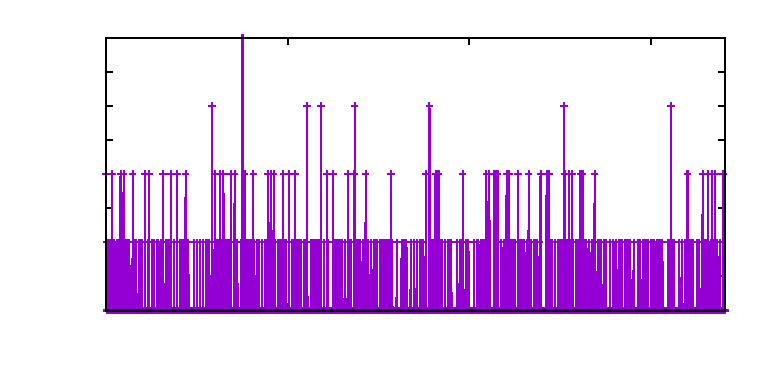
\includegraphics{cpuloadx1}}%
    \gplfronttext
  \end{picture}%
\endgroup

		\caption{i5}
	\end{subfigure}
	\begin{subfigure}{1\textwidth}
		% GNUPLOT: LaTeX picture with Postscript
\begingroup
  \makeatletter
  \providecommand\color[2][]{%
    \GenericError{(gnuplot) \space\space\space\@spaces}{%
      Package color not loaded in conjunction with
      terminal option `colourtext'%
    }{See the gnuplot documentation for explanation.%
    }{Either use 'blacktext' in gnuplot or load the package
      color.sty in LaTeX.}%
    \renewcommand\color[2][]{}%
  }%
  \providecommand\includegraphics[2][]{%
    \GenericError{(gnuplot) \space\space\space\@spaces}{%
      Package graphicx or graphics not loaded%
    }{See the gnuplot documentation for explanation.%
    }{The gnuplot epslatex terminal needs graphicx.sty or graphics.sty.}%
    \renewcommand\includegraphics[2][]{}%
  }%
  \providecommand\rotatebox[2]{#2}%
  \@ifundefined{ifGPcolor}{%
    \newif\ifGPcolor
    \GPcolorfalse
  }{}%
  \@ifundefined{ifGPblacktext}{%
    \newif\ifGPblacktext
    \GPblacktexttrue
  }{}%
  % define a \g@addto@macro without @ in the name:
  \let\gplgaddtomacro\g@addto@macro
  % define empty templates for all commands taking text:
  \gdef\gplbacktext{}%
  \gdef\gplfronttext{}%
  \makeatother
  \ifGPblacktext
    % no textcolor at all
    \def\colorrgb#1{}%
    \def\colorgray#1{}%
  \else
    % gray or color?
    \ifGPcolor
      \def\colorrgb#1{\color[rgb]{#1}}%
      \def\colorgray#1{\color[gray]{#1}}%
      \expandafter\def\csname LTw\endcsname{\color{white}}%
      \expandafter\def\csname LTb\endcsname{\color{black}}%
      \expandafter\def\csname LTa\endcsname{\color{black}}%
      \expandafter\def\csname LT0\endcsname{\color[rgb]{1,0,0}}%
      \expandafter\def\csname LT1\endcsname{\color[rgb]{0,1,0}}%
      \expandafter\def\csname LT2\endcsname{\color[rgb]{0,0,1}}%
      \expandafter\def\csname LT3\endcsname{\color[rgb]{1,0,1}}%
      \expandafter\def\csname LT4\endcsname{\color[rgb]{0,1,1}}%
      \expandafter\def\csname LT5\endcsname{\color[rgb]{1,1,0}}%
      \expandafter\def\csname LT6\endcsname{\color[rgb]{0,0,0}}%
      \expandafter\def\csname LT7\endcsname{\color[rgb]{1,0.3,0}}%
      \expandafter\def\csname LT8\endcsname{\color[rgb]{0.5,0.5,0.5}}%
    \else
      % gray
      \def\colorrgb#1{\color{black}}%
      \def\colorgray#1{\color[gray]{#1}}%
      \expandafter\def\csname LTw\endcsname{\color{white}}%
      \expandafter\def\csname LTb\endcsname{\color{black}}%
      \expandafter\def\csname LTa\endcsname{\color{black}}%
      \expandafter\def\csname LT0\endcsname{\color{black}}%
      \expandafter\def\csname LT1\endcsname{\color{black}}%
      \expandafter\def\csname LT2\endcsname{\color{black}}%
      \expandafter\def\csname LT3\endcsname{\color{black}}%
      \expandafter\def\csname LT4\endcsname{\color{black}}%
      \expandafter\def\csname LT5\endcsname{\color{black}}%
      \expandafter\def\csname LT6\endcsname{\color{black}}%
      \expandafter\def\csname LT7\endcsname{\color{black}}%
      \expandafter\def\csname LT8\endcsname{\color{black}}%
    \fi
  \fi
    \setlength{\unitlength}{0.0500bp}%
    \ifx\gptboxheight\undefined%
      \newlength{\gptboxheight}%
      \newlength{\gptboxwidth}%
      \newsavebox{\gptboxtext}%
    \fi%
    \setlength{\fboxrule}{0.5pt}%
    \setlength{\fboxsep}{1pt}%
\begin{picture}(7200.00,3276.00)%
    \gplgaddtomacro\gplbacktext{%
      \csname LTb\endcsname%%
      \put(726,440){\makebox(0,0)[r]{\strut{}0.00}}%
      \put(726,963){\makebox(0,0)[r]{\strut{}0.20}}%
      \put(726,1486){\makebox(0,0)[r]{\strut{}0.40}}%
      \put(726,2009){\makebox(0,0)[r]{\strut{}0.60}}%
      \put(726,2532){\makebox(0,0)[r]{\strut{}0.80}}%
      \put(726,3055){\makebox(0,0)[r]{\strut{}1.00}}%
      \put(858,220){\makebox(0,0){\strut{}0}}%
      \put(2601,220){\makebox(0,0){\strut{}10}}%
      \put(4343,220){\makebox(0,0){\strut{}20}}%
      \put(6086,220){\makebox(0,0){\strut{}30}}%
    }%
    \gplgaddtomacro\gplfronttext{%
    }%
    \gplbacktext
    \put(0,0){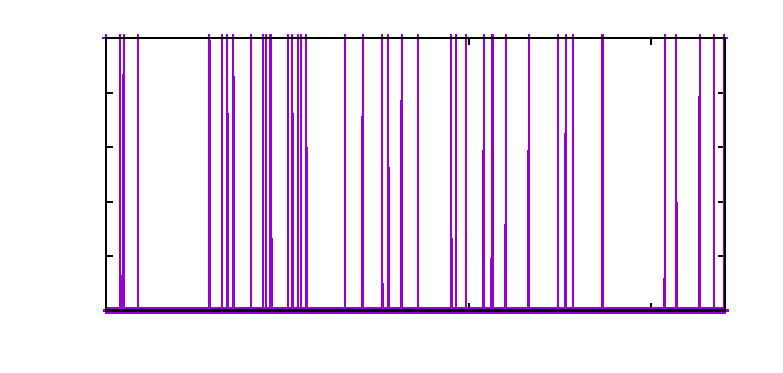
\includegraphics{cpuload-desktop}}%
    \gplfronttext
  \end{picture}%
\endgroup

		\caption{i7}
	\end{subfigure}
	\begin{subfigure}{1\textwidth}
		% GNUPLOT: LaTeX picture with Postscript
\begingroup
  \makeatletter
  \providecommand\color[2][]{%
    \GenericError{(gnuplot) \space\space\space\@spaces}{%
      Package color not loaded in conjunction with
      terminal option `colourtext'%
    }{See the gnuplot documentation for explanation.%
    }{Either use 'blacktext' in gnuplot or load the package
      color.sty in LaTeX.}%
    \renewcommand\color[2][]{}%
  }%
  \providecommand\includegraphics[2][]{%
    \GenericError{(gnuplot) \space\space\space\@spaces}{%
      Package graphicx or graphics not loaded%
    }{See the gnuplot documentation for explanation.%
    }{The gnuplot epslatex terminal needs graphicx.sty or graphics.sty.}%
    \renewcommand\includegraphics[2][]{}%
  }%
  \providecommand\rotatebox[2]{#2}%
  \@ifundefined{ifGPcolor}{%
    \newif\ifGPcolor
    \GPcolorfalse
  }{}%
  \@ifundefined{ifGPblacktext}{%
    \newif\ifGPblacktext
    \GPblacktexttrue
  }{}%
  % define a \g@addto@macro without @ in the name:
  \let\gplgaddtomacro\g@addto@macro
  % define empty templates for all commands taking text:
  \gdef\gplbacktext{}%
  \gdef\gplfronttext{}%
  \makeatother
  \ifGPblacktext
    % no textcolor at all
    \def\colorrgb#1{}%
    \def\colorgray#1{}%
  \else
    % gray or color?
    \ifGPcolor
      \def\colorrgb#1{\color[rgb]{#1}}%
      \def\colorgray#1{\color[gray]{#1}}%
      \expandafter\def\csname LTw\endcsname{\color{white}}%
      \expandafter\def\csname LTb\endcsname{\color{black}}%
      \expandafter\def\csname LTa\endcsname{\color{black}}%
      \expandafter\def\csname LT0\endcsname{\color[rgb]{1,0,0}}%
      \expandafter\def\csname LT1\endcsname{\color[rgb]{0,1,0}}%
      \expandafter\def\csname LT2\endcsname{\color[rgb]{0,0,1}}%
      \expandafter\def\csname LT3\endcsname{\color[rgb]{1,0,1}}%
      \expandafter\def\csname LT4\endcsname{\color[rgb]{0,1,1}}%
      \expandafter\def\csname LT5\endcsname{\color[rgb]{1,1,0}}%
      \expandafter\def\csname LT6\endcsname{\color[rgb]{0,0,0}}%
      \expandafter\def\csname LT7\endcsname{\color[rgb]{1,0.3,0}}%
      \expandafter\def\csname LT8\endcsname{\color[rgb]{0.5,0.5,0.5}}%
    \else
      % gray
      \def\colorrgb#1{\color{black}}%
      \def\colorgray#1{\color[gray]{#1}}%
      \expandafter\def\csname LTw\endcsname{\color{white}}%
      \expandafter\def\csname LTb\endcsname{\color{black}}%
      \expandafter\def\csname LTa\endcsname{\color{black}}%
      \expandafter\def\csname LT0\endcsname{\color{black}}%
      \expandafter\def\csname LT1\endcsname{\color{black}}%
      \expandafter\def\csname LT2\endcsname{\color{black}}%
      \expandafter\def\csname LT3\endcsname{\color{black}}%
      \expandafter\def\csname LT4\endcsname{\color{black}}%
      \expandafter\def\csname LT5\endcsname{\color{black}}%
      \expandafter\def\csname LT6\endcsname{\color{black}}%
      \expandafter\def\csname LT7\endcsname{\color{black}}%
      \expandafter\def\csname LT8\endcsname{\color{black}}%
    \fi
  \fi
    \setlength{\unitlength}{0.0500bp}%
    \ifx\gptboxheight\undefined%
      \newlength{\gptboxheight}%
      \newlength{\gptboxwidth}%
      \newsavebox{\gptboxtext}%
    \fi%
    \setlength{\fboxrule}{0.5pt}%
    \setlength{\fboxsep}{1pt}%
\begin{picture}(7200.00,3276.00)%
    \gplgaddtomacro\gplbacktext{%
      \csname LTb\endcsname%%
      \put(726,440){\makebox(0,0)[r]{\strut{}0.00}}%
      \put(726,814){\makebox(0,0)[r]{\strut{}1.00}}%
      \put(726,1187){\makebox(0,0)[r]{\strut{}2.00}}%
      \put(726,1561){\makebox(0,0)[r]{\strut{}3.00}}%
      \put(726,1934){\makebox(0,0)[r]{\strut{}4.00}}%
      \put(726,2308){\makebox(0,0)[r]{\strut{}5.00}}%
      \put(726,2681){\makebox(0,0)[r]{\strut{}6.00}}%
      \put(726,3055){\makebox(0,0)[r]{\strut{}7.00}}%
      \put(858,220){\makebox(0,0){\strut{}0}}%
      \put(3498,220){\makebox(0,0){\strut{}10}}%
      \put(6139,220){\makebox(0,0){\strut{}20}}%
    }%
    \gplgaddtomacro\gplfronttext{%
    }%
    \gplbacktext
    \put(0,0){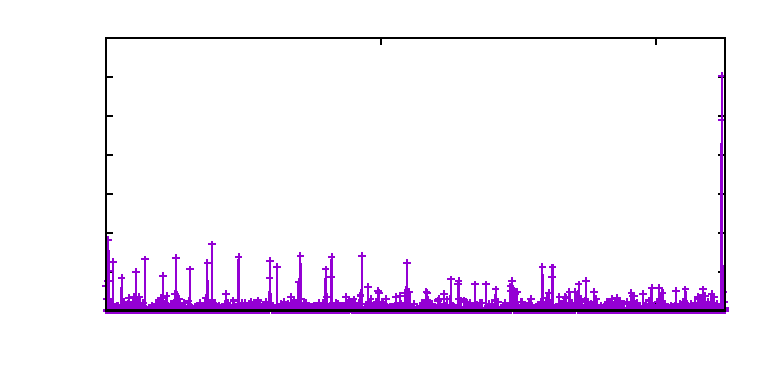
\includegraphics{cpuload-server}}%
    \gplfronttext
  \end{picture}%
\endgroup

		\caption{Xeon}
	\end{subfigure}
	\caption{CPU baselines for benchmarks. The x-axes show CPU load in
	percent, as reported by the operating system (100\% load corresponds to
	all cores being busy 100\% of the time). The y-axes show time in
	minutes. Please note that both axes differ between the plots.}
	\label{fig:cpuload}
\end{figure}

\subsection{Degrees of parallelism}

\begin{code}
\begin{Verbatim}[frame=single]
  let taskCount parallel tasks do {
    final int startIndex = ...;
      double sum = 0.0;
      int k = startIndex;
      for (int j=0; j < workPerThread; j++){
        if(k<arraySize - 1){
          ++k;
        } else {
          k=0;
        }
        sum += array[indices[k]];
      }
  }
\end{Verbatim}
	\caption{Simplified code for the memory-bound parallelism experiment.}
\end{code}

\begin{code}
\begin{Verbatim}[frame=single]
  let taskCount parallel tasks do {
    double d = Double.MAX_VALUE;
    for (long j = 0; j < workPerThread; ++j) {
      d /= divisor;
    }
  }
\end{Verbatim}
	\caption{Simplified code for the CPU-bound parallelism experiment.}
\end{code}

\begin{figure}[hbpt]
\graphicspath{{plots/}}
% GNUPLOT: LaTeX picture with Postscript
\begingroup
  \makeatletter
  \providecommand\color[2][]{%
    \GenericError{(gnuplot) \space\space\space\@spaces}{%
      Package color not loaded in conjunction with
      terminal option `colourtext'%
    }{See the gnuplot documentation for explanation.%
    }{Either use 'blacktext' in gnuplot or load the package
      color.sty in LaTeX.}%
    \renewcommand\color[2][]{}%
  }%
  \providecommand\includegraphics[2][]{%
    \GenericError{(gnuplot) \space\space\space\@spaces}{%
      Package graphicx or graphics not loaded%
    }{See the gnuplot documentation for explanation.%
    }{The gnuplot epslatex terminal needs graphicx.sty or graphics.sty.}%
    \renewcommand\includegraphics[2][]{}%
  }%
  \providecommand\rotatebox[2]{#2}%
  \@ifundefined{ifGPcolor}{%
    \newif\ifGPcolor
    \GPcolorfalse
  }{}%
  \@ifundefined{ifGPblacktext}{%
    \newif\ifGPblacktext
    \GPblacktexttrue
  }{}%
  % define a \g@addto@macro without @ in the name:
  \let\gplgaddtomacro\g@addto@macro
  % define empty templates for all commands taking text:
  \gdef\gplbacktext{}%
  \gdef\gplfronttext{}%
  \makeatother
  \ifGPblacktext
    % no textcolor at all
    \def\colorrgb#1{}%
    \def\colorgray#1{}%
  \else
    % gray or color?
    \ifGPcolor
      \def\colorrgb#1{\color[rgb]{#1}}%
      \def\colorgray#1{\color[gray]{#1}}%
      \expandafter\def\csname LTw\endcsname{\color{white}}%
      \expandafter\def\csname LTb\endcsname{\color{black}}%
      \expandafter\def\csname LTa\endcsname{\color{black}}%
      \expandafter\def\csname LT0\endcsname{\color[rgb]{1,0,0}}%
      \expandafter\def\csname LT1\endcsname{\color[rgb]{0,1,0}}%
      \expandafter\def\csname LT2\endcsname{\color[rgb]{0,0,1}}%
      \expandafter\def\csname LT3\endcsname{\color[rgb]{1,0,1}}%
      \expandafter\def\csname LT4\endcsname{\color[rgb]{0,1,1}}%
      \expandafter\def\csname LT5\endcsname{\color[rgb]{1,1,0}}%
      \expandafter\def\csname LT6\endcsname{\color[rgb]{0,0,0}}%
      \expandafter\def\csname LT7\endcsname{\color[rgb]{1,0.3,0}}%
      \expandafter\def\csname LT8\endcsname{\color[rgb]{0.5,0.5,0.5}}%
    \else
      % gray
      \def\colorrgb#1{\color{black}}%
      \def\colorgray#1{\color[gray]{#1}}%
      \expandafter\def\csname LTw\endcsname{\color{white}}%
      \expandafter\def\csname LTb\endcsname{\color{black}}%
      \expandafter\def\csname LTa\endcsname{\color{black}}%
      \expandafter\def\csname LT0\endcsname{\color{black}}%
      \expandafter\def\csname LT1\endcsname{\color{black}}%
      \expandafter\def\csname LT2\endcsname{\color{black}}%
      \expandafter\def\csname LT3\endcsname{\color{black}}%
      \expandafter\def\csname LT4\endcsname{\color{black}}%
      \expandafter\def\csname LT5\endcsname{\color{black}}%
      \expandafter\def\csname LT6\endcsname{\color{black}}%
      \expandafter\def\csname LT7\endcsname{\color{black}}%
      \expandafter\def\csname LT8\endcsname{\color{black}}%
    \fi
  \fi
    \setlength{\unitlength}{0.0500bp}%
    \ifx\gptboxheight\undefined%
      \newlength{\gptboxheight}%
      \newlength{\gptboxwidth}%
      \newsavebox{\gptboxtext}%
    \fi%
    \setlength{\fboxrule}{0.5pt}%
    \setlength{\fboxsep}{1pt}%
\begin{picture}(7200.00,5040.00)%
    \gplgaddtomacro\gplbacktext{%
      \csname LTb\endcsname%%
      \put(528,406){\makebox(0,0)[r]{\strut{}$0$}}%
      \put(528,958){\makebox(0,0)[r]{\strut{}$5\times10^{7}$}}%
      \put(528,1509){\makebox(0,0)[r]{\strut{}$1\times10^{8}$}}%
      \put(528,2061){\makebox(0,0)[r]{\strut{}$1.5\times10^{8}$}}%
      \put(528,2613){\makebox(0,0)[r]{\strut{}$2\times10^{8}$}}%
      \put(528,3164){\makebox(0,0)[r]{\strut{}$2.5\times10^{8}$}}%
      \put(528,3716){\makebox(0,0)[r]{\strut{}$3\times10^{8}$}}%
      \put(528,4267){\makebox(0,0)[r]{\strut{}$3.5\times10^{8}$}}%
      \put(528,4819){\makebox(0,0)[r]{\strut{}$4\times10^{8}$}}%
      \put(660,274){\rotatebox{-45}{\makebox(0,0)[l]{\strut{}1}}}%
      \put(1313,274){\rotatebox{-45}{\makebox(0,0)[l]{\strut{}2}}}%
      \put(1966,274){\rotatebox{-45}{\makebox(0,0)[l]{\strut{}3}}}%
      \put(2620,274){\rotatebox{-45}{\makebox(0,0)[l]{\strut{}4}}}%
      \put(3273,274){\rotatebox{-45}{\makebox(0,0)[l]{\strut{}5}}}%
      \put(3926,274){\rotatebox{-45}{\makebox(0,0)[l]{\strut{}6}}}%
      \put(4579,274){\rotatebox{-45}{\makebox(0,0)[l]{\strut{}7}}}%
      \put(5233,274){\rotatebox{-45}{\makebox(0,0)[l]{\strut{}8}}}%
      \put(5886,274){\rotatebox{-45}{\makebox(0,0)[l]{\strut{}9}}}%
      \put(6539,274){\rotatebox{-45}{\makebox(0,0)[l]{\strut{}10}}}%
    }%
    \gplgaddtomacro\gplfronttext{%
      \csname LTb\endcsname%%
      \put(2112,4646){\makebox(0,0)[r]{\strut{}mem-reads}}%
      \csname LTb\endcsname%%
      \put(2112,4426){\makebox(0,0)[r]{\strut{}mem-writes}}%
      \csname LTb\endcsname%%
      \put(2112,4206){\makebox(0,0)[r]{\strut{}CPU}}%
      \csname LTb\endcsname%%
      \put(2112,3986){\makebox(0,0)[r]{\strut{}mixed}}%
    }%
    \gplbacktext
    \put(0,0){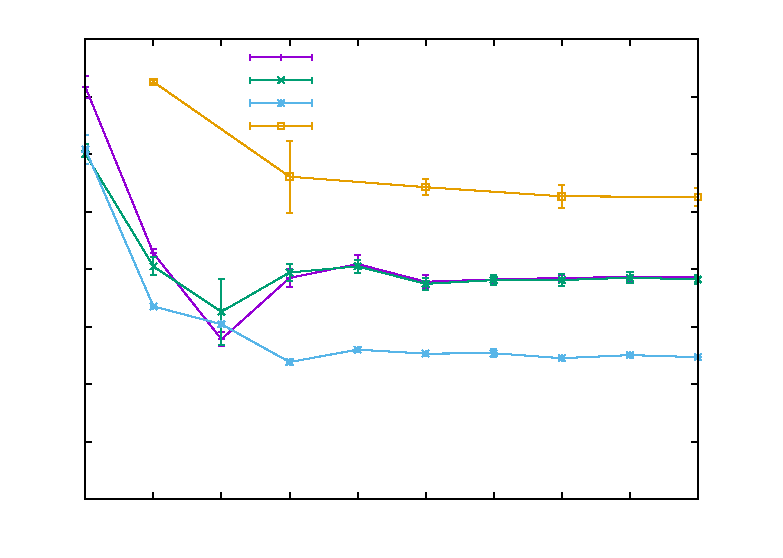
\includegraphics{paral}}%
    \gplfronttext
  \end{picture}%
\endgroup

	\caption{Parallelism experiment on the i5 platform. The plot shows
	wall-clock execution time in ns., as a function of thread count.}
	\label{fig:parallel-i5}
\end{figure}

\begin{figure}[hbpt]
\graphicspath{{plots/}}
% GNUPLOT: LaTeX picture with Postscript
\begingroup
  \makeatletter
  \providecommand\color[2][]{%
    \GenericError{(gnuplot) \space\space\space\@spaces}{%
      Package color not loaded in conjunction with
      terminal option `colourtext'%
    }{See the gnuplot documentation for explanation.%
    }{Either use 'blacktext' in gnuplot or load the package
      color.sty in LaTeX.}%
    \renewcommand\color[2][]{}%
  }%
  \providecommand\includegraphics[2][]{%
    \GenericError{(gnuplot) \space\space\space\@spaces}{%
      Package graphicx or graphics not loaded%
    }{See the gnuplot documentation for explanation.%
    }{The gnuplot epslatex terminal needs graphicx.sty or graphics.sty.}%
    \renewcommand\includegraphics[2][]{}%
  }%
  \providecommand\rotatebox[2]{#2}%
  \@ifundefined{ifGPcolor}{%
    \newif\ifGPcolor
    \GPcolorfalse
  }{}%
  \@ifundefined{ifGPblacktext}{%
    \newif\ifGPblacktext
    \GPblacktexttrue
  }{}%
  % define a \g@addto@macro without @ in the name:
  \let\gplgaddtomacro\g@addto@macro
  % define empty templates for all commands taking text:
  \gdef\gplbacktext{}%
  \gdef\gplfronttext{}%
  \makeatother
  \ifGPblacktext
    % no textcolor at all
    \def\colorrgb#1{}%
    \def\colorgray#1{}%
  \else
    % gray or color?
    \ifGPcolor
      \def\colorrgb#1{\color[rgb]{#1}}%
      \def\colorgray#1{\color[gray]{#1}}%
      \expandafter\def\csname LTw\endcsname{\color{white}}%
      \expandafter\def\csname LTb\endcsname{\color{black}}%
      \expandafter\def\csname LTa\endcsname{\color{black}}%
      \expandafter\def\csname LT0\endcsname{\color[rgb]{1,0,0}}%
      \expandafter\def\csname LT1\endcsname{\color[rgb]{0,1,0}}%
      \expandafter\def\csname LT2\endcsname{\color[rgb]{0,0,1}}%
      \expandafter\def\csname LT3\endcsname{\color[rgb]{1,0,1}}%
      \expandafter\def\csname LT4\endcsname{\color[rgb]{0,1,1}}%
      \expandafter\def\csname LT5\endcsname{\color[rgb]{1,1,0}}%
      \expandafter\def\csname LT6\endcsname{\color[rgb]{0,0,0}}%
      \expandafter\def\csname LT7\endcsname{\color[rgb]{1,0.3,0}}%
      \expandafter\def\csname LT8\endcsname{\color[rgb]{0.5,0.5,0.5}}%
    \else
      % gray
      \def\colorrgb#1{\color{black}}%
      \def\colorgray#1{\color[gray]{#1}}%
      \expandafter\def\csname LTw\endcsname{\color{white}}%
      \expandafter\def\csname LTb\endcsname{\color{black}}%
      \expandafter\def\csname LTa\endcsname{\color{black}}%
      \expandafter\def\csname LT0\endcsname{\color{black}}%
      \expandafter\def\csname LT1\endcsname{\color{black}}%
      \expandafter\def\csname LT2\endcsname{\color{black}}%
      \expandafter\def\csname LT3\endcsname{\color{black}}%
      \expandafter\def\csname LT4\endcsname{\color{black}}%
      \expandafter\def\csname LT5\endcsname{\color{black}}%
      \expandafter\def\csname LT6\endcsname{\color{black}}%
      \expandafter\def\csname LT7\endcsname{\color{black}}%
      \expandafter\def\csname LT8\endcsname{\color{black}}%
    \fi
  \fi
    \setlength{\unitlength}{0.0500bp}%
    \ifx\gptboxheight\undefined%
      \newlength{\gptboxheight}%
      \newlength{\gptboxwidth}%
      \newsavebox{\gptboxtext}%
    \fi%
    \setlength{\fboxrule}{0.5pt}%
    \setlength{\fboxsep}{1pt}%
\begin{picture}(7200.00,5040.00)%
    \gplgaddtomacro\gplbacktext{%
      \csname LTb\endcsname%%
      \put(528,406){\makebox(0,0)[r]{\strut{}$0$}}%
      \put(528,1142){\makebox(0,0)[r]{\strut{}$1\times10^{8}$}}%
      \put(528,1877){\makebox(0,0)[r]{\strut{}$2\times10^{8}$}}%
      \put(528,2613){\makebox(0,0)[r]{\strut{}$3\times10^{8}$}}%
      \put(528,3348){\makebox(0,0)[r]{\strut{}$4\times10^{8}$}}%
      \put(528,4084){\makebox(0,0)[r]{\strut{}$5\times10^{8}$}}%
      \put(528,4819){\makebox(0,0)[r]{\strut{}$6\times10^{8}$}}%
      \put(660,274){\rotatebox{-45}{\makebox(0,0)[l]{\strut{}1}}}%
      \put(1313,274){\rotatebox{-45}{\makebox(0,0)[l]{\strut{}2}}}%
      \put(1966,274){\rotatebox{-45}{\makebox(0,0)[l]{\strut{}3}}}%
      \put(2620,274){\rotatebox{-45}{\makebox(0,0)[l]{\strut{}4}}}%
      \put(3273,274){\rotatebox{-45}{\makebox(0,0)[l]{\strut{}5}}}%
      \put(3926,274){\rotatebox{-45}{\makebox(0,0)[l]{\strut{}6}}}%
      \put(4579,274){\rotatebox{-45}{\makebox(0,0)[l]{\strut{}7}}}%
      \put(5233,274){\rotatebox{-45}{\makebox(0,0)[l]{\strut{}8}}}%
      \put(5886,274){\rotatebox{-45}{\makebox(0,0)[l]{\strut{}9}}}%
      \put(6539,274){\rotatebox{-45}{\makebox(0,0)[l]{\strut{}10}}}%
    }%
    \gplgaddtomacro\gplfronttext{%
      \csname LTb\endcsname%%
      \put(2112,4646){\makebox(0,0)[r]{\strut{}mem-reads}}%
      \csname LTb\endcsname%%
      \put(2112,4426){\makebox(0,0)[r]{\strut{}mem-writes}}%
      \csname LTb\endcsname%%
      \put(2112,4206){\makebox(0,0)[r]{\strut{}CPU}}%
      \csname LTb\endcsname%%
      \put(2112,3986){\makebox(0,0)[r]{\strut{}mixed}}%
    }%
    \gplbacktext
    \put(0,0){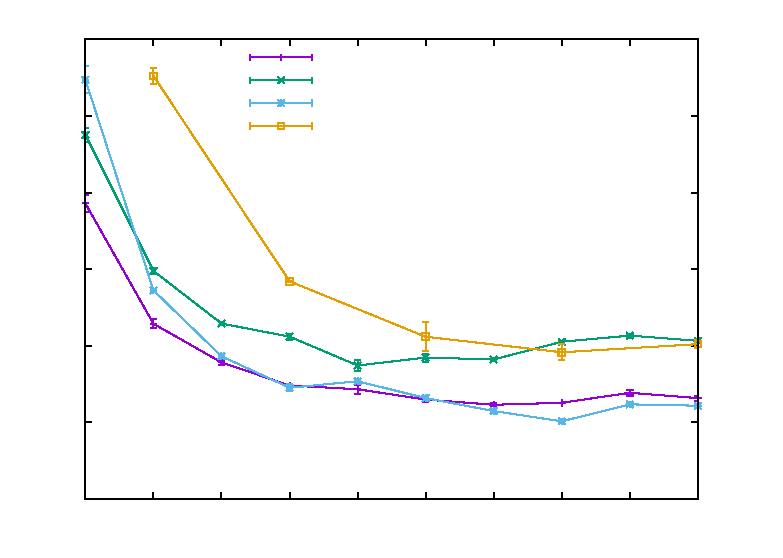
\includegraphics{paral-desktop}}%
    \gplfronttext
  \end{picture}%
\endgroup

	\caption{Parallelism experiment on the i7 platform. The plot shows
	wall-clock execution time in ns., as a function of thread count.}
	\label{fig:parallel-i7}
\end{figure}

\begin{figure}[hbpt]
\graphicspath{{plots/}}
% GNUPLOT: LaTeX picture with Postscript
\begingroup
  \makeatletter
  \providecommand\color[2][]{%
    \GenericError{(gnuplot) \space\space\space\@spaces}{%
      Package color not loaded in conjunction with
      terminal option `colourtext'%
    }{See the gnuplot documentation for explanation.%
    }{Either use 'blacktext' in gnuplot or load the package
      color.sty in LaTeX.}%
    \renewcommand\color[2][]{}%
  }%
  \providecommand\includegraphics[2][]{%
    \GenericError{(gnuplot) \space\space\space\@spaces}{%
      Package graphicx or graphics not loaded%
    }{See the gnuplot documentation for explanation.%
    }{The gnuplot epslatex terminal needs graphicx.sty or graphics.sty.}%
    \renewcommand\includegraphics[2][]{}%
  }%
  \providecommand\rotatebox[2]{#2}%
  \@ifundefined{ifGPcolor}{%
    \newif\ifGPcolor
    \GPcolorfalse
  }{}%
  \@ifundefined{ifGPblacktext}{%
    \newif\ifGPblacktext
    \GPblacktexttrue
  }{}%
  % define a \g@addto@macro without @ in the name:
  \let\gplgaddtomacro\g@addto@macro
  % define empty templates for all commands taking text:
  \gdef\gplbacktext{}%
  \gdef\gplfronttext{}%
  \makeatother
  \ifGPblacktext
    % no textcolor at all
    \def\colorrgb#1{}%
    \def\colorgray#1{}%
  \else
    % gray or color?
    \ifGPcolor
      \def\colorrgb#1{\color[rgb]{#1}}%
      \def\colorgray#1{\color[gray]{#1}}%
      \expandafter\def\csname LTw\endcsname{\color{white}}%
      \expandafter\def\csname LTb\endcsname{\color{black}}%
      \expandafter\def\csname LTa\endcsname{\color{black}}%
      \expandafter\def\csname LT0\endcsname{\color[rgb]{1,0,0}}%
      \expandafter\def\csname LT1\endcsname{\color[rgb]{0,1,0}}%
      \expandafter\def\csname LT2\endcsname{\color[rgb]{0,0,1}}%
      \expandafter\def\csname LT3\endcsname{\color[rgb]{1,0,1}}%
      \expandafter\def\csname LT4\endcsname{\color[rgb]{0,1,1}}%
      \expandafter\def\csname LT5\endcsname{\color[rgb]{1,1,0}}%
      \expandafter\def\csname LT6\endcsname{\color[rgb]{0,0,0}}%
      \expandafter\def\csname LT7\endcsname{\color[rgb]{1,0.3,0}}%
      \expandafter\def\csname LT8\endcsname{\color[rgb]{0.5,0.5,0.5}}%
    \else
      % gray
      \def\colorrgb#1{\color{black}}%
      \def\colorgray#1{\color[gray]{#1}}%
      \expandafter\def\csname LTw\endcsname{\color{white}}%
      \expandafter\def\csname LTb\endcsname{\color{black}}%
      \expandafter\def\csname LTa\endcsname{\color{black}}%
      \expandafter\def\csname LT0\endcsname{\color{black}}%
      \expandafter\def\csname LT1\endcsname{\color{black}}%
      \expandafter\def\csname LT2\endcsname{\color{black}}%
      \expandafter\def\csname LT3\endcsname{\color{black}}%
      \expandafter\def\csname LT4\endcsname{\color{black}}%
      \expandafter\def\csname LT5\endcsname{\color{black}}%
      \expandafter\def\csname LT6\endcsname{\color{black}}%
      \expandafter\def\csname LT7\endcsname{\color{black}}%
      \expandafter\def\csname LT8\endcsname{\color{black}}%
    \fi
  \fi
    \setlength{\unitlength}{0.0500bp}%
    \ifx\gptboxheight\undefined%
      \newlength{\gptboxheight}%
      \newlength{\gptboxwidth}%
      \newsavebox{\gptboxtext}%
    \fi%
    \setlength{\fboxrule}{0.5pt}%
    \setlength{\fboxsep}{1pt}%
\begin{picture}(7200.00,5040.00)%
    \gplgaddtomacro\gplbacktext{%
      \csname LTb\endcsname%%
      \put(528,406){\makebox(0,0)[r]{\strut{}$0$}}%
      \put(528,847){\makebox(0,0)[r]{\strut{}$5\times10^{8}$}}%
      \put(528,1289){\makebox(0,0)[r]{\strut{}$1\times10^{9}$}}%
      \put(528,1730){\makebox(0,0)[r]{\strut{}$1.5\times10^{9}$}}%
      \put(528,2171){\makebox(0,0)[r]{\strut{}$2\times10^{9}$}}%
      \put(528,2613){\makebox(0,0)[r]{\strut{}$2.5\times10^{9}$}}%
      \put(528,3054){\makebox(0,0)[r]{\strut{}$3\times10^{9}$}}%
      \put(528,3495){\makebox(0,0)[r]{\strut{}$3.5\times10^{9}$}}%
      \put(528,3936){\makebox(0,0)[r]{\strut{}$4\times10^{9}$}}%
      \put(528,4378){\makebox(0,0)[r]{\strut{}$4.5\times10^{9}$}}%
      \put(528,4819){\makebox(0,0)[r]{\strut{}$5\times10^{9}$}}%
      \put(660,274){\rotatebox{-45}{\makebox(0,0)[l]{\strut{}1}}}%
      \put(753,274){\rotatebox{-45}{\makebox(0,0)[l]{\strut{}2}}}%
      \put(940,274){\rotatebox{-45}{\makebox(0,0)[l]{\strut{}4}}}%
      \put(1313,274){\rotatebox{-45}{\makebox(0,0)[l]{\strut{}8}}}%
      \put(1686,274){\rotatebox{-45}{\makebox(0,0)[l]{\strut{}12}}}%
      \put(2060,274){\rotatebox{-45}{\makebox(0,0)[l]{\strut{}16}}}%
      \put(2806,274){\rotatebox{-45}{\makebox(0,0)[l]{\strut{}24}}}%
      \put(3553,274){\rotatebox{-45}{\makebox(0,0)[l]{\strut{}32}}}%
      \put(5046,274){\rotatebox{-45}{\makebox(0,0)[l]{\strut{}48}}}%
      \put(6539,274){\rotatebox{-45}{\makebox(0,0)[l]{\strut{}64}}}%
    }%
    \gplgaddtomacro\gplfronttext{%
      \csname LTb\endcsname%%
      \put(2112,4646){\makebox(0,0)[r]{\strut{}mem-reads}}%
      \csname LTb\endcsname%%
      \put(2112,4426){\makebox(0,0)[r]{\strut{}mem-writes}}%
      \csname LTb\endcsname%%
      \put(2112,4206){\makebox(0,0)[r]{\strut{}CPU}}%
      \csname LTb\endcsname%%
      \put(2112,3986){\makebox(0,0)[r]{\strut{}mixed}}%
    }%
    \gplbacktext
    \put(0,0){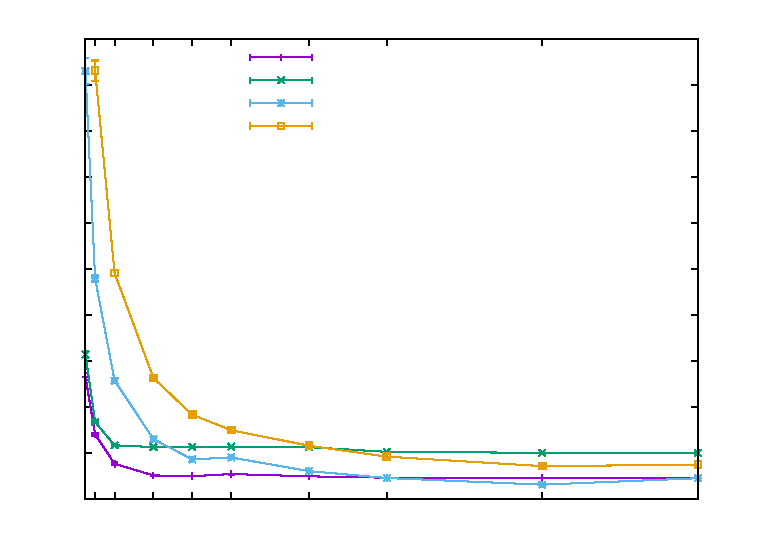
\includegraphics{paral-server}}%
    \gplfronttext
  \end{picture}%
\endgroup

	\caption{Parallelism experiment on the Xeon platform. The plot shows
	wall-clock execution time in ns., as a function of thread count.}
	\label{fig:parallel-xeon}
\end{figure}

\subsection{Memory hierarchy access-times}
\begin{code}
\begin{Verbatim}[frame=single]
  private static double jumps(int[] arr) {
    int k = 0;
    for(int j = 0; j < 1 << 25; ++j){
      k = arr[k];
    }
    return k;
  }
\end{Verbatim}
	\caption{Code for measuring memory access times.}
\end{code}

\begin{figure}[hbpt]
	\graphicspath{{plots/}}
	\begin{subfigure}{1\textwidth}
		% GNUPLOT: LaTeX picture with Postscript
\begingroup
  \makeatletter
  \providecommand\color[2][]{%
    \GenericError{(gnuplot) \space\space\space\@spaces}{%
      Package color not loaded in conjunction with
      terminal option `colourtext'%
    }{See the gnuplot documentation for explanation.%
    }{Either use 'blacktext' in gnuplot or load the package
      color.sty in LaTeX.}%
    \renewcommand\color[2][]{}%
  }%
  \providecommand\includegraphics[2][]{%
    \GenericError{(gnuplot) \space\space\space\@spaces}{%
      Package graphicx or graphics not loaded%
    }{See the gnuplot documentation for explanation.%
    }{The gnuplot epslatex terminal needs graphicx.sty or graphics.sty.}%
    \renewcommand\includegraphics[2][]{}%
  }%
  \providecommand\rotatebox[2]{#2}%
  \@ifundefined{ifGPcolor}{%
    \newif\ifGPcolor
    \GPcolorfalse
  }{}%
  \@ifundefined{ifGPblacktext}{%
    \newif\ifGPblacktext
    \GPblacktexttrue
  }{}%
  % define a \g@addto@macro without @ in the name:
  \let\gplgaddtomacro\g@addto@macro
  % define empty templates for all commands taking text:
  \gdef\gplbacktext{}%
  \gdef\gplfronttext{}%
  \makeatother
  \ifGPblacktext
    % no textcolor at all
    \def\colorrgb#1{}%
    \def\colorgray#1{}%
  \else
    % gray or color?
    \ifGPcolor
      \def\colorrgb#1{\color[rgb]{#1}}%
      \def\colorgray#1{\color[gray]{#1}}%
      \expandafter\def\csname LTw\endcsname{\color{white}}%
      \expandafter\def\csname LTb\endcsname{\color{black}}%
      \expandafter\def\csname LTa\endcsname{\color{black}}%
      \expandafter\def\csname LT0\endcsname{\color[rgb]{1,0,0}}%
      \expandafter\def\csname LT1\endcsname{\color[rgb]{0,1,0}}%
      \expandafter\def\csname LT2\endcsname{\color[rgb]{0,0,1}}%
      \expandafter\def\csname LT3\endcsname{\color[rgb]{1,0,1}}%
      \expandafter\def\csname LT4\endcsname{\color[rgb]{0,1,1}}%
      \expandafter\def\csname LT5\endcsname{\color[rgb]{1,1,0}}%
      \expandafter\def\csname LT6\endcsname{\color[rgb]{0,0,0}}%
      \expandafter\def\csname LT7\endcsname{\color[rgb]{1,0.3,0}}%
      \expandafter\def\csname LT8\endcsname{\color[rgb]{0.5,0.5,0.5}}%
    \else
      % gray
      \def\colorrgb#1{\color{black}}%
      \def\colorgray#1{\color[gray]{#1}}%
      \expandafter\def\csname LTw\endcsname{\color{white}}%
      \expandafter\def\csname LTb\endcsname{\color{black}}%
      \expandafter\def\csname LTa\endcsname{\color{black}}%
      \expandafter\def\csname LT0\endcsname{\color{black}}%
      \expandafter\def\csname LT1\endcsname{\color{black}}%
      \expandafter\def\csname LT2\endcsname{\color{black}}%
      \expandafter\def\csname LT3\endcsname{\color{black}}%
      \expandafter\def\csname LT4\endcsname{\color{black}}%
      \expandafter\def\csname LT5\endcsname{\color{black}}%
      \expandafter\def\csname LT6\endcsname{\color{black}}%
      \expandafter\def\csname LT7\endcsname{\color{black}}%
      \expandafter\def\csname LT8\endcsname{\color{black}}%
    \fi
  \fi
    \setlength{\unitlength}{0.0500bp}%
    \ifx\gptboxheight\undefined%
      \newlength{\gptboxheight}%
      \newlength{\gptboxwidth}%
      \newsavebox{\gptboxtext}%
    \fi%
    \setlength{\fboxrule}{0.5pt}%
    \setlength{\fboxsep}{1pt}%
\begin{picture}(7200.00,3880.80)%
    \gplgaddtomacro\gplbacktext{%
      \csname LTb\endcsname%%
      \put(528,500){\makebox(0,0)[r]{\strut{}$0$}}%
      \put(528,816){\makebox(0,0)[r]{\strut{}$2$}}%
      \put(528,1132){\makebox(0,0)[r]{\strut{}$4$}}%
      \put(528,1448){\makebox(0,0)[r]{\strut{}$6$}}%
      \put(528,1764){\makebox(0,0)[r]{\strut{}$8$}}%
      \put(528,2080){\makebox(0,0)[r]{\strut{}$10$}}%
      \put(528,2396){\makebox(0,0)[r]{\strut{}$12$}}%
      \put(528,2712){\makebox(0,0)[r]{\strut{}$14$}}%
      \put(528,3028){\makebox(0,0)[r]{\strut{}$16$}}%
      \put(528,3344){\makebox(0,0)[r]{\strut{}$18$}}%
      \put(528,3660){\makebox(0,0)[r]{\strut{}$20$}}%
      \put(752,368){\rotatebox{-45}{\makebox(0,0)[l]{\strut{}8}}}%
      \put(844,368){\rotatebox{-45}{\makebox(0,0)[l]{\strut{}16}}}%
      \put(1027,368){\rotatebox{-45}{\makebox(0,0)[l]{\strut{}32}}}%
      \put(1395,368){\rotatebox{-45}{\makebox(0,0)[l]{\strut{}64}}}%
      \put(2130,368){\rotatebox{-45}{\makebox(0,0)[l]{\strut{}128}}}%
      \put(3600,368){\rotatebox{-45}{\makebox(0,0)[l]{\strut{}256}}}%
      \put(6539,368){\rotatebox{-45}{\makebox(0,0)[l]{\strut{}512}}}%
    }%
    \gplgaddtomacro\gplfronttext{%
      \csname LTb\endcsname%%
      \put(5552,3487){\makebox(0,0)[r]{\strut{}readtimes-by-array-size}}%
      \csname LTb\endcsname%%
      \put(5552,3267){\makebox(0,0)[r]{\strut{}readtimes-by-array-size-padded}}%
      \csname LTb\endcsname%%
      \put(5552,3047){\makebox(0,0)[r]{\strut{}readtimes-by-array-size-desktop}}%
      \csname LTb\endcsname%%
      \put(5552,2827){\makebox(0,0)[r]{\strut{}readtimes-by-array-size-padded-desktop}}%
      \csname LTb\endcsname%%
      \put(5552,2607){\makebox(0,0)[r]{\strut{}readtimes-by-array-size-server}}%
      \csname LTb\endcsname%%
      \put(5552,2387){\makebox(0,0)[r]{\strut{}readtimes-by-array-size-padded-server}}%
    }%
    \gplbacktext
    \put(0,0){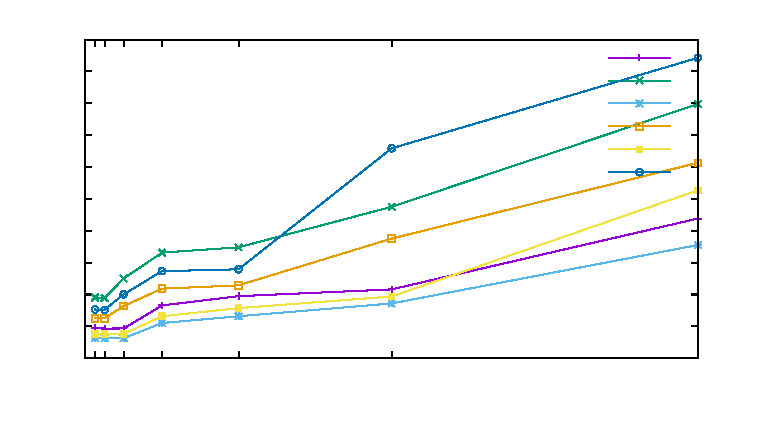
\includegraphics{readtimes}}%
    \gplfronttext
  \end{picture}%
\endgroup

	\end{subfigure}
	\begin{subfigure}{1\textwidth}
		% GNUPLOT: LaTeX picture with Postscript
\begingroup
  \makeatletter
  \providecommand\color[2][]{%
    \GenericError{(gnuplot) \space\space\space\@spaces}{%
      Package color not loaded in conjunction with
      terminal option `colourtext'%
    }{See the gnuplot documentation for explanation.%
    }{Either use 'blacktext' in gnuplot or load the package
      color.sty in LaTeX.}%
    \renewcommand\color[2][]{}%
  }%
  \providecommand\includegraphics[2][]{%
    \GenericError{(gnuplot) \space\space\space\@spaces}{%
      Package graphicx or graphics not loaded%
    }{See the gnuplot documentation for explanation.%
    }{The gnuplot epslatex terminal needs graphicx.sty or graphics.sty.}%
    \renewcommand\includegraphics[2][]{}%
  }%
  \providecommand\rotatebox[2]{#2}%
  \@ifundefined{ifGPcolor}{%
    \newif\ifGPcolor
    \GPcolorfalse
  }{}%
  \@ifundefined{ifGPblacktext}{%
    \newif\ifGPblacktext
    \GPblacktexttrue
  }{}%
  % define a \g@addto@macro without @ in the name:
  \let\gplgaddtomacro\g@addto@macro
  % define empty templates for all commands taking text:
  \gdef\gplbacktext{}%
  \gdef\gplfronttext{}%
  \makeatother
  \ifGPblacktext
    % no textcolor at all
    \def\colorrgb#1{}%
    \def\colorgray#1{}%
  \else
    % gray or color?
    \ifGPcolor
      \def\colorrgb#1{\color[rgb]{#1}}%
      \def\colorgray#1{\color[gray]{#1}}%
      \expandafter\def\csname LTw\endcsname{\color{white}}%
      \expandafter\def\csname LTb\endcsname{\color{black}}%
      \expandafter\def\csname LTa\endcsname{\color{black}}%
      \expandafter\def\csname LT0\endcsname{\color[rgb]{1,0,0}}%
      \expandafter\def\csname LT1\endcsname{\color[rgb]{0,1,0}}%
      \expandafter\def\csname LT2\endcsname{\color[rgb]{0,0,1}}%
      \expandafter\def\csname LT3\endcsname{\color[rgb]{1,0,1}}%
      \expandafter\def\csname LT4\endcsname{\color[rgb]{0,1,1}}%
      \expandafter\def\csname LT5\endcsname{\color[rgb]{1,1,0}}%
      \expandafter\def\csname LT6\endcsname{\color[rgb]{0,0,0}}%
      \expandafter\def\csname LT7\endcsname{\color[rgb]{1,0.3,0}}%
      \expandafter\def\csname LT8\endcsname{\color[rgb]{0.5,0.5,0.5}}%
    \else
      % gray
      \def\colorrgb#1{\color{black}}%
      \def\colorgray#1{\color[gray]{#1}}%
      \expandafter\def\csname LTw\endcsname{\color{white}}%
      \expandafter\def\csname LTb\endcsname{\color{black}}%
      \expandafter\def\csname LTa\endcsname{\color{black}}%
      \expandafter\def\csname LT0\endcsname{\color{black}}%
      \expandafter\def\csname LT1\endcsname{\color{black}}%
      \expandafter\def\csname LT2\endcsname{\color{black}}%
      \expandafter\def\csname LT3\endcsname{\color{black}}%
      \expandafter\def\csname LT4\endcsname{\color{black}}%
      \expandafter\def\csname LT5\endcsname{\color{black}}%
      \expandafter\def\csname LT6\endcsname{\color{black}}%
      \expandafter\def\csname LT7\endcsname{\color{black}}%
      \expandafter\def\csname LT8\endcsname{\color{black}}%
    \fi
  \fi
    \setlength{\unitlength}{0.0500bp}%
    \ifx\gptboxheight\undefined%
      \newlength{\gptboxheight}%
      \newlength{\gptboxwidth}%
      \newsavebox{\gptboxtext}%
    \fi%
    \setlength{\fboxrule}{0.5pt}%
    \setlength{\fboxsep}{1pt}%
\begin{picture}(7200.00,3780.00)%
    \gplgaddtomacro\gplbacktext{%
      \csname LTb\endcsname%%
      \put(528,593){\makebox(0,0)[r]{\strut{}$0$}}%
      \put(528,890){\makebox(0,0)[r]{\strut{}$5$}}%
      \put(528,1186){\makebox(0,0)[r]{\strut{}$10$}}%
      \put(528,1483){\makebox(0,0)[r]{\strut{}$15$}}%
      \put(528,1779){\makebox(0,0)[r]{\strut{}$20$}}%
      \put(528,2076){\makebox(0,0)[r]{\strut{}$25$}}%
      \put(528,2373){\makebox(0,0)[r]{\strut{}$30$}}%
      \put(528,2669){\makebox(0,0)[r]{\strut{}$35$}}%
      \put(528,2966){\makebox(0,0)[r]{\strut{}$40$}}%
      \put(528,3262){\makebox(0,0)[r]{\strut{}$45$}}%
      \put(528,3559){\makebox(0,0)[r]{\strut{}$50$}}%
      \put(660,461){\rotatebox{-45}{\makebox(0,0)[l]{\strut{}512}}}%
      \put(1052,461){\rotatebox{-45}{\makebox(0,0)[l]{\strut{}1024}}}%
      \put(1836,461){\rotatebox{-45}{\makebox(0,0)[l]{\strut{}2048}}}%
      \put(2620,461){\rotatebox{-45}{\makebox(0,0)[l]{\strut{}3072}}}%
      \put(3404,461){\rotatebox{-45}{\makebox(0,0)[l]{\strut{}4096}}}%
      \put(6539,461){\rotatebox{-45}{\makebox(0,0)[l]{\strut{}8192}}}%
    }%
    \gplgaddtomacro\gplfronttext{%
      \csname LTb\endcsname%%
      \put(5552,3386){\makebox(0,0)[r]{\strut{}i5}}%
      \csname LTb\endcsname%%
      \put(5552,3166){\makebox(0,0)[r]{\strut{}padded-i5}}%
      \csname LTb\endcsname%%
      \put(5552,2946){\makebox(0,0)[r]{\strut{}i7}}%
      \csname LTb\endcsname%%
      \put(5552,2726){\makebox(0,0)[r]{\strut{}padded-i7}}%
      \csname LTb\endcsname%%
      \put(5552,2506){\makebox(0,0)[r]{\strut{}Xeon}}%
      \csname LTb\endcsname%%
      \put(5552,2286){\makebox(0,0)[r]{\strut{}padded-Xeon}}%
    }%
    \gplbacktext
    \put(0,0){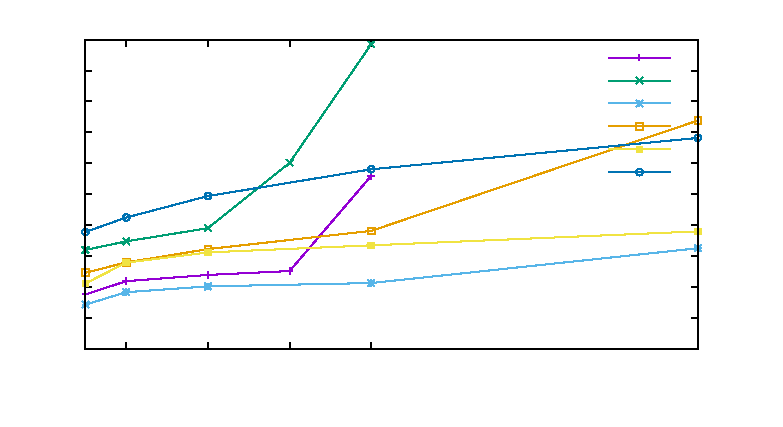
\includegraphics{readtimes2}}%
    \gplfronttext
  \end{picture}%
\endgroup

	\end{subfigure}
	\begin{subfigure}{1\textwidth}
		% GNUPLOT: LaTeX picture with Postscript
\begingroup
  \makeatletter
  \providecommand\color[2][]{%
    \GenericError{(gnuplot) \space\space\space\@spaces}{%
      Package color not loaded in conjunction with
      terminal option `colourtext'%
    }{See the gnuplot documentation for explanation.%
    }{Either use 'blacktext' in gnuplot or load the package
      color.sty in LaTeX.}%
    \renewcommand\color[2][]{}%
  }%
  \providecommand\includegraphics[2][]{%
    \GenericError{(gnuplot) \space\space\space\@spaces}{%
      Package graphicx or graphics not loaded%
    }{See the gnuplot documentation for explanation.%
    }{The gnuplot epslatex terminal needs graphicx.sty or graphics.sty.}%
    \renewcommand\includegraphics[2][]{}%
  }%
  \providecommand\rotatebox[2]{#2}%
  \@ifundefined{ifGPcolor}{%
    \newif\ifGPcolor
    \GPcolorfalse
  }{}%
  \@ifundefined{ifGPblacktext}{%
    \newif\ifGPblacktext
    \GPblacktexttrue
  }{}%
  % define a \g@addto@macro without @ in the name:
  \let\gplgaddtomacro\g@addto@macro
  % define empty templates for all commands taking text:
  \gdef\gplbacktext{}%
  \gdef\gplfronttext{}%
  \makeatother
  \ifGPblacktext
    % no textcolor at all
    \def\colorrgb#1{}%
    \def\colorgray#1{}%
  \else
    % gray or color?
    \ifGPcolor
      \def\colorrgb#1{\color[rgb]{#1}}%
      \def\colorgray#1{\color[gray]{#1}}%
      \expandafter\def\csname LTw\endcsname{\color{white}}%
      \expandafter\def\csname LTb\endcsname{\color{black}}%
      \expandafter\def\csname LTa\endcsname{\color{black}}%
      \expandafter\def\csname LT0\endcsname{\color[rgb]{1,0,0}}%
      \expandafter\def\csname LT1\endcsname{\color[rgb]{0,1,0}}%
      \expandafter\def\csname LT2\endcsname{\color[rgb]{0,0,1}}%
      \expandafter\def\csname LT3\endcsname{\color[rgb]{1,0,1}}%
      \expandafter\def\csname LT4\endcsname{\color[rgb]{0,1,1}}%
      \expandafter\def\csname LT5\endcsname{\color[rgb]{1,1,0}}%
      \expandafter\def\csname LT6\endcsname{\color[rgb]{0,0,0}}%
      \expandafter\def\csname LT7\endcsname{\color[rgb]{1,0.3,0}}%
      \expandafter\def\csname LT8\endcsname{\color[rgb]{0.5,0.5,0.5}}%
    \else
      % gray
      \def\colorrgb#1{\color{black}}%
      \def\colorgray#1{\color[gray]{#1}}%
      \expandafter\def\csname LTw\endcsname{\color{white}}%
      \expandafter\def\csname LTb\endcsname{\color{black}}%
      \expandafter\def\csname LTa\endcsname{\color{black}}%
      \expandafter\def\csname LT0\endcsname{\color{black}}%
      \expandafter\def\csname LT1\endcsname{\color{black}}%
      \expandafter\def\csname LT2\endcsname{\color{black}}%
      \expandafter\def\csname LT3\endcsname{\color{black}}%
      \expandafter\def\csname LT4\endcsname{\color{black}}%
      \expandafter\def\csname LT5\endcsname{\color{black}}%
      \expandafter\def\csname LT6\endcsname{\color{black}}%
      \expandafter\def\csname LT7\endcsname{\color{black}}%
      \expandafter\def\csname LT8\endcsname{\color{black}}%
    \fi
  \fi
    \setlength{\unitlength}{0.0500bp}%
    \ifx\gptboxheight\undefined%
      \newlength{\gptboxheight}%
      \newlength{\gptboxwidth}%
      \newsavebox{\gptboxtext}%
    \fi%
    \setlength{\fboxrule}{0.5pt}%
    \setlength{\fboxsep}{1pt}%
\begin{picture}(7200.00,3880.80)%
    \gplgaddtomacro\gplbacktext{%
      \csname LTb\endcsname%%
      \put(528,686){\makebox(0,0)[r]{\strut{}$0$}}%
      \put(528,1111){\makebox(0,0)[r]{\strut{}$20$}}%
      \put(528,1536){\makebox(0,0)[r]{\strut{}$40$}}%
      \put(528,1961){\makebox(0,0)[r]{\strut{}$60$}}%
      \put(528,2385){\makebox(0,0)[r]{\strut{}$80$}}%
      \put(528,2810){\makebox(0,0)[r]{\strut{}$100$}}%
      \put(528,3235){\makebox(0,0)[r]{\strut{}$120$}}%
      \put(528,3660){\makebox(0,0)[r]{\strut{}$140$}}%
      \put(660,554){\rotatebox{-45}{\makebox(0,0)[l]{\strut{}8192}}}%
      \put(1500,554){\rotatebox{-45}{\makebox(0,0)[l]{\strut{}16384}}}%
      \put(3180,554){\rotatebox{-45}{\makebox(0,0)[l]{\strut{}32768}}}%
      \put(6119,554){\rotatebox{-45}{\makebox(0,0)[l]{\strut{}61440}}}%
      \put(6539,554){\rotatebox{-45}{\makebox(0,0)[l]{\strut{}65536}}}%
    }%
    \gplgaddtomacro\gplfronttext{%
      \csname LTb\endcsname%%
      \put(5552,3487){\makebox(0,0)[r]{\strut{}readtimes-by-array-size-desktop}}%
      \csname LTb\endcsname%%
      \put(5552,3267){\makebox(0,0)[r]{\strut{}readtimes-by-array-size-padded-desktop}}%
      \csname LTb\endcsname%%
      \put(5552,3047){\makebox(0,0)[r]{\strut{}readtimes-by-array-size-server}}%
      \csname LTb\endcsname%%
      \put(5552,2827){\makebox(0,0)[r]{\strut{}readtimes-by-array-size-padded-server}}%
    }%
    \gplbacktext
    \put(0,0){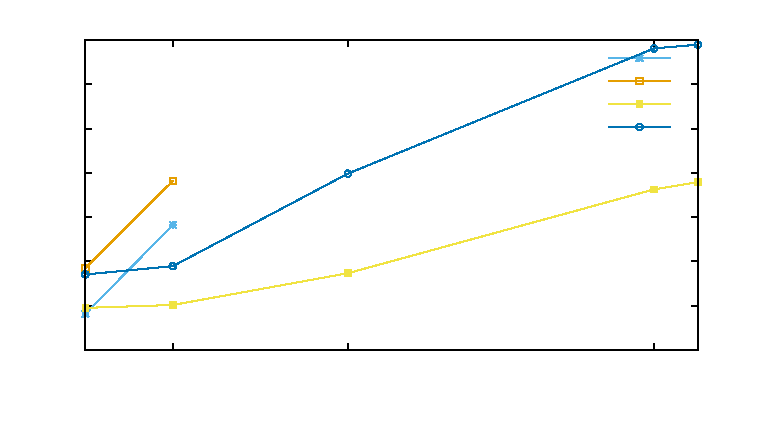
\includegraphics{readtimes3}}%
    \gplfronttext
  \end{picture}%
\endgroup

	\end{subfigure}
	\caption{Random cyclic reads, approximating memory-access times on all 3
	platforms. The y-axes show the average time per read operation, measured
	over $2^{25}$ reads. The x-axes show the working-set size in KiB.}
	\label{fig:readtimes}
\end{figure}

\section{Multicore cache performance}

To see the possible impact of false sharing, it is illustrative to look at a
few contrived example programs. In this section we look at a handful of
variations of programs that perform simple operations in a multicore
setting.

\subsection{Uncontended writes}
The first example we examine illustrates the impact of false sharing by running
simple, uncontended, integer-field increment operations in parallel threads. To see
the impact of false sharing, we observe the time it takes to perform an
increment as a function of the distance between the fields in memory.

\begin{code}
\begin{Verbatim}[frame=single]
  let taskCount parallel tasks do {
    Counter cc = ...;
    for (long i = 0; i < increments_per_thread; i++) {
      cc.value++;
    }
  }
\end{Verbatim}
	\caption{Simplified code for the local-field version of the uncontended-writes
	experiment.}
\end{code}

Each thread performs millions of increments. The fields are
uncontended; each thread has its own integer-field and performs no read or write
operations to fields used by the other threads. Since each thread operates on
its own field, there is no need for synchronization. Nonetheless, we perform
the experiment in variants with and without \java{volatile} integer declarations, to
see the performance impact in both cases.

Since the fiends are uncontended, we will assume the difference in performance
to be a result of unnecessary coherence operations due to false sharing.

In the experiments with volatile integers, each thread performs 6M increments.
In the experiments without volatile, each thread performs 66M increments. 
Figure \ref{fig:uncont} and \ref{fig:uncont-nob} show the average time per
increment, as a function of padding.

\begin{figure}[hbpt]
\graphicspath{{plots/}}
% GNUPLOT: LaTeX picture with Postscript
\begingroup
  \makeatletter
  \providecommand\color[2][]{%
    \GenericError{(gnuplot) \space\space\space\@spaces}{%
      Package color not loaded in conjunction with
      terminal option `colourtext'%
    }{See the gnuplot documentation for explanation.%
    }{Either use 'blacktext' in gnuplot or load the package
      color.sty in LaTeX.}%
    \renewcommand\color[2][]{}%
  }%
  \providecommand\includegraphics[2][]{%
    \GenericError{(gnuplot) \space\space\space\@spaces}{%
      Package graphicx or graphics not loaded%
    }{See the gnuplot documentation for explanation.%
    }{The gnuplot epslatex terminal needs graphicx.sty or graphics.sty.}%
    \renewcommand\includegraphics[2][]{}%
  }%
  \providecommand\rotatebox[2]{#2}%
  \@ifundefined{ifGPcolor}{%
    \newif\ifGPcolor
    \GPcolorfalse
  }{}%
  \@ifundefined{ifGPblacktext}{%
    \newif\ifGPblacktext
    \GPblacktexttrue
  }{}%
  % define a \g@addto@macro without @ in the name:
  \let\gplgaddtomacro\g@addto@macro
  % define empty templates for all commands taking text:
  \gdef\gplbacktext{}%
  \gdef\gplfronttext{}%
  \makeatother
  \ifGPblacktext
    % no textcolor at all
    \def\colorrgb#1{}%
    \def\colorgray#1{}%
  \else
    % gray or color?
    \ifGPcolor
      \def\colorrgb#1{\color[rgb]{#1}}%
      \def\colorgray#1{\color[gray]{#1}}%
      \expandafter\def\csname LTw\endcsname{\color{white}}%
      \expandafter\def\csname LTb\endcsname{\color{black}}%
      \expandafter\def\csname LTa\endcsname{\color{black}}%
      \expandafter\def\csname LT0\endcsname{\color[rgb]{1,0,0}}%
      \expandafter\def\csname LT1\endcsname{\color[rgb]{0,1,0}}%
      \expandafter\def\csname LT2\endcsname{\color[rgb]{0,0,1}}%
      \expandafter\def\csname LT3\endcsname{\color[rgb]{1,0,1}}%
      \expandafter\def\csname LT4\endcsname{\color[rgb]{0,1,1}}%
      \expandafter\def\csname LT5\endcsname{\color[rgb]{1,1,0}}%
      \expandafter\def\csname LT6\endcsname{\color[rgb]{0,0,0}}%
      \expandafter\def\csname LT7\endcsname{\color[rgb]{1,0.3,0}}%
      \expandafter\def\csname LT8\endcsname{\color[rgb]{0.5,0.5,0.5}}%
    \else
      % gray
      \def\colorrgb#1{\color{black}}%
      \def\colorgray#1{\color[gray]{#1}}%
      \expandafter\def\csname LTw\endcsname{\color{white}}%
      \expandafter\def\csname LTb\endcsname{\color{black}}%
      \expandafter\def\csname LTa\endcsname{\color{black}}%
      \expandafter\def\csname LT0\endcsname{\color{black}}%
      \expandafter\def\csname LT1\endcsname{\color{black}}%
      \expandafter\def\csname LT2\endcsname{\color{black}}%
      \expandafter\def\csname LT3\endcsname{\color{black}}%
      \expandafter\def\csname LT4\endcsname{\color{black}}%
      \expandafter\def\csname LT5\endcsname{\color{black}}%
      \expandafter\def\csname LT6\endcsname{\color{black}}%
      \expandafter\def\csname LT7\endcsname{\color{black}}%
      \expandafter\def\csname LT8\endcsname{\color{black}}%
    \fi
  \fi
    \setlength{\unitlength}{0.0500bp}%
    \ifx\gptboxheight\undefined%
      \newlength{\gptboxheight}%
      \newlength{\gptboxwidth}%
      \newsavebox{\gptboxtext}%
    \fi%
    \setlength{\fboxrule}{0.5pt}%
    \setlength{\fboxsep}{1pt}%
\begin{picture}(7200.00,5040.00)%
    \gplgaddtomacro\gplbacktext{%
      \csname LTb\endcsname%%
      \put(1122,440){\makebox(0,0)[r]{\strut{}$0$}}%
      \put(1122,878){\makebox(0,0)[r]{\strut{}$2\times10^{8}$}}%
      \put(1122,1316){\makebox(0,0)[r]{\strut{}$4\times10^{8}$}}%
      \put(1122,1754){\makebox(0,0)[r]{\strut{}$6\times10^{8}$}}%
      \put(1122,2192){\makebox(0,0)[r]{\strut{}$8\times10^{8}$}}%
      \put(1122,2630){\makebox(0,0)[r]{\strut{}$1\times10^{9}$}}%
      \put(1122,3067){\makebox(0,0)[r]{\strut{}$1.2\times10^{9}$}}%
      \put(1122,3505){\makebox(0,0)[r]{\strut{}$1.4\times10^{9}$}}%
      \put(1122,3943){\makebox(0,0)[r]{\strut{}$1.6\times10^{9}$}}%
      \put(1122,4381){\makebox(0,0)[r]{\strut{}$1.8\times10^{9}$}}%
      \put(1122,4819){\makebox(0,0)[r]{\strut{}$2\times10^{9}$}}%
      \put(1254,220){\makebox(0,0){\strut{}0}}%
      \put(1427,220){\makebox(0,0){\strut{}4}}%
      \put(1601,220){\makebox(0,0){\strut{}8}}%
      \put(1948,220){\makebox(0,0){\strut{}16}}%
      \put(2641,220){\makebox(0,0){\strut{}32}}%
      \put(4029,220){\makebox(0,0){\strut{}64}}%
      \put(6803,220){\makebox(0,0){\strut{}128}}%
    }%
    \gplgaddtomacro\gplfronttext{%
      \csname LTb\endcsname%%
      \put(5816,4646){\makebox(0,0)[r]{\strut{}i5-local}}%
      \csname LTb\endcsname%%
      \put(5816,4426){\makebox(0,0)[r]{\strut{}i5-array}}%
      \csname LTb\endcsname%%
      \put(5816,4206){\makebox(0,0)[r]{\strut{}i7-local}}%
      \csname LTb\endcsname%%
      \put(5816,3986){\makebox(0,0)[r]{\strut{}i7-array}}%
      \csname LTb\endcsname%%
      \put(5816,3766){\makebox(0,0)[r]{\strut{}xeon-local}}%
      \csname LTb\endcsname%%
      \put(5816,3546){\makebox(0,0)[r]{\strut{}xeon-array}}%
    }%
    \gplbacktext
    \put(0,0){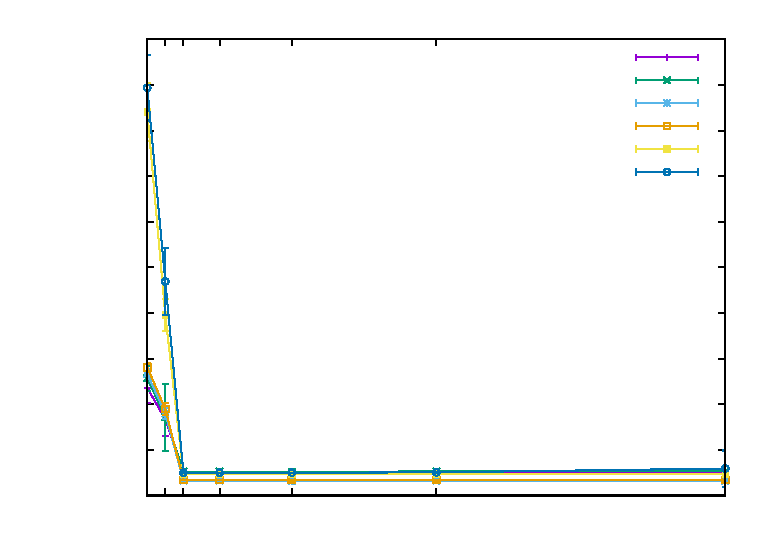
\includegraphics{barrier}}%
    \gplfronttext
  \end{picture}%
\endgroup

\caption{Uncontended increments on volatile integers. The plot shows wall-clock
	execution time, as a function of the number of bytes used as padding
	between the integers.}
	\label{fig:uncont}
\end{figure}

\begin{figure}[hbpt]
\graphicspath{{plots/}}
% GNUPLOT: LaTeX picture with Postscript
\begingroup
  \makeatletter
  \providecommand\color[2][]{%
    \GenericError{(gnuplot) \space\space\space\@spaces}{%
      Package color not loaded in conjunction with
      terminal option `colourtext'%
    }{See the gnuplot documentation for explanation.%
    }{Either use 'blacktext' in gnuplot or load the package
      color.sty in LaTeX.}%
    \renewcommand\color[2][]{}%
  }%
  \providecommand\includegraphics[2][]{%
    \GenericError{(gnuplot) \space\space\space\@spaces}{%
      Package graphicx or graphics not loaded%
    }{See the gnuplot documentation for explanation.%
    }{The gnuplot epslatex terminal needs graphicx.sty or graphics.sty.}%
    \renewcommand\includegraphics[2][]{}%
  }%
  \providecommand\rotatebox[2]{#2}%
  \@ifundefined{ifGPcolor}{%
    \newif\ifGPcolor
    \GPcolorfalse
  }{}%
  \@ifundefined{ifGPblacktext}{%
    \newif\ifGPblacktext
    \GPblacktexttrue
  }{}%
  % define a \g@addto@macro without @ in the name:
  \let\gplgaddtomacro\g@addto@macro
  % define empty templates for all commands taking text:
  \gdef\gplbacktext{}%
  \gdef\gplfronttext{}%
  \makeatother
  \ifGPblacktext
    % no textcolor at all
    \def\colorrgb#1{}%
    \def\colorgray#1{}%
  \else
    % gray or color?
    \ifGPcolor
      \def\colorrgb#1{\color[rgb]{#1}}%
      \def\colorgray#1{\color[gray]{#1}}%
      \expandafter\def\csname LTw\endcsname{\color{white}}%
      \expandafter\def\csname LTb\endcsname{\color{black}}%
      \expandafter\def\csname LTa\endcsname{\color{black}}%
      \expandafter\def\csname LT0\endcsname{\color[rgb]{1,0,0}}%
      \expandafter\def\csname LT1\endcsname{\color[rgb]{0,1,0}}%
      \expandafter\def\csname LT2\endcsname{\color[rgb]{0,0,1}}%
      \expandafter\def\csname LT3\endcsname{\color[rgb]{1,0,1}}%
      \expandafter\def\csname LT4\endcsname{\color[rgb]{0,1,1}}%
      \expandafter\def\csname LT5\endcsname{\color[rgb]{1,1,0}}%
      \expandafter\def\csname LT6\endcsname{\color[rgb]{0,0,0}}%
      \expandafter\def\csname LT7\endcsname{\color[rgb]{1,0.3,0}}%
      \expandafter\def\csname LT8\endcsname{\color[rgb]{0.5,0.5,0.5}}%
    \else
      % gray
      \def\colorrgb#1{\color{black}}%
      \def\colorgray#1{\color[gray]{#1}}%
      \expandafter\def\csname LTw\endcsname{\color{white}}%
      \expandafter\def\csname LTb\endcsname{\color{black}}%
      \expandafter\def\csname LTa\endcsname{\color{black}}%
      \expandafter\def\csname LT0\endcsname{\color{black}}%
      \expandafter\def\csname LT1\endcsname{\color{black}}%
      \expandafter\def\csname LT2\endcsname{\color{black}}%
      \expandafter\def\csname LT3\endcsname{\color{black}}%
      \expandafter\def\csname LT4\endcsname{\color{black}}%
      \expandafter\def\csname LT5\endcsname{\color{black}}%
      \expandafter\def\csname LT6\endcsname{\color{black}}%
      \expandafter\def\csname LT7\endcsname{\color{black}}%
      \expandafter\def\csname LT8\endcsname{\color{black}}%
    \fi
  \fi
    \setlength{\unitlength}{0.0500bp}%
    \ifx\gptboxheight\undefined%
      \newlength{\gptboxheight}%
      \newlength{\gptboxwidth}%
      \newsavebox{\gptboxtext}%
    \fi%
    \setlength{\fboxrule}{0.5pt}%
    \setlength{\fboxsep}{1pt}%
\begin{picture}(7200.00,5040.00)%
    \gplgaddtomacro\gplbacktext{%
      \csname LTb\endcsname%%
      \put(858,440){\makebox(0,0)[r]{\strut{}$0$}}%
      \put(858,1170){\makebox(0,0)[r]{\strut{}$1\times10^{9}$}}%
      \put(858,1900){\makebox(0,0)[r]{\strut{}$2\times10^{9}$}}%
      \put(858,2630){\makebox(0,0)[r]{\strut{}$3\times10^{9}$}}%
      \put(858,3359){\makebox(0,0)[r]{\strut{}$4\times10^{9}$}}%
      \put(858,4089){\makebox(0,0)[r]{\strut{}$5\times10^{9}$}}%
      \put(858,4819){\makebox(0,0)[r]{\strut{}$6\times10^{9}$}}%
      \put(990,220){\makebox(0,0){\strut{}0}}%
      \put(1172,220){\makebox(0,0){\strut{}4}}%
      \put(1353,220){\makebox(0,0){\strut{}8}}%
      \put(1717,220){\makebox(0,0){\strut{}16}}%
      \put(2443,220){\makebox(0,0){\strut{}32}}%
      \put(3897,220){\makebox(0,0){\strut{}64}}%
      \put(6803,220){\makebox(0,0){\strut{}128}}%
    }%
    \gplgaddtomacro\gplfronttext{%
    }%
    \gplbacktext
    \put(0,0){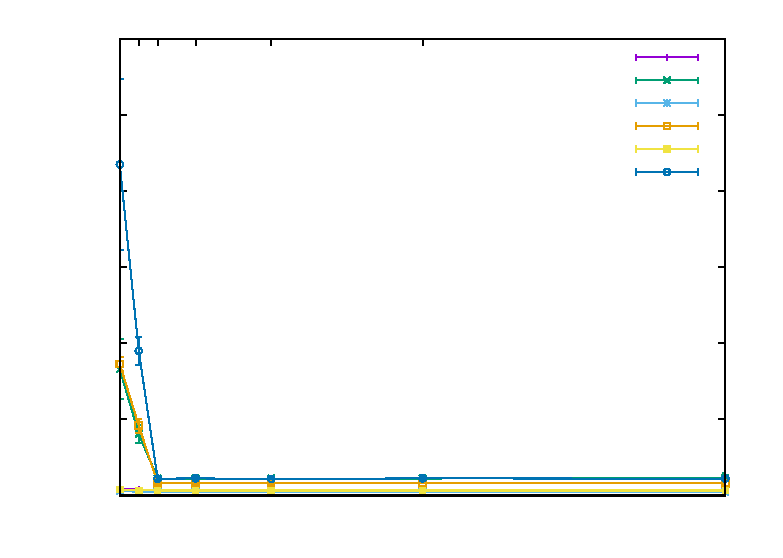
\includegraphics{nobarrier}}%
    \gplfronttext
  \end{picture}%
\endgroup

\caption{Uncontended increments on non-volatile integers. The plot shows
	wall-clock execution time, as a function of the number of bytes used as padding
	between the integers.}
\label{fig:uncont-nob}
\end{figure}

\mynote{Add explanation of the different plots (array/local,
barrier/no-barrier), include values of plots (plots are hard to read), and
reflect/conclude}

\subsection{Contended writes}

In the previous section we examined the performance of uncontended memory
operations to see the existence and cost of false sharing. In this section, we
shall see that observing the performance of contended memory operations - where
coherence overhead is strictly necessary - can be just as illustrative.

\begin{code}
\begin{Verbatim}[frame=single]
  int sharedInt = 0;
  let taskCount parallel tasks do {
    for (long j = 0; j < increments_per_thread; ++j) {
      sharedInt++;
    }
  }
\end{Verbatim}
	\caption{Simplified code for the local-field version of the contended-writes
	experiment.}
\end{code}

The program is similar to \mynote{reference uncontended snippet}, but in this
version all threads operate on a single, shared integer field. As in the previous
section, we run two versions of the experiment: One where the field is
\java{volatile}, and one where it is not. As this experiment uses a shared field,
there is no need to store it in an array. However, benchmarks using a
single-element array are included, to show that the behaviour is not
significantly affected by this change.

An additional experiment is included here, running an additional thread that
only reads the integer field. This allows us to see that, perhaps contrary to
intuition, read operations in a multicore setting also incur a coherency
overhead.

\mynote{include getter/stop code snippet}

We need the reading thread to run for the full duration of the experiment. To
that end, the thread does not perform a predetermined number of operations, but
is started before the others, and terminated only when the others are
finished. This incurs an overhead, as the thread needs to be stopped before the
benchmark finishes! However, an additional experiment has shown that the time it
takes to stop a thread is far too small to significantly skew our results.

\mynote{include table of numbers (they are 833.4$\pm$2.82 (desktop),
1940.5$\pm$58.12 (server),
and 1256.7$\pm$13.59 (laptop) ns)})

\begin{figure}[hbpt]
	\graphicspath{{plots/}}
	\begin{subfigure}{0.5\textwidth}
		% GNUPLOT: LaTeX picture with Postscript
\begingroup
  \makeatletter
  \providecommand\color[2][]{%
    \GenericError{(gnuplot) \space\space\space\@spaces}{%
      Package color not loaded in conjunction with
      terminal option `colourtext'%
    }{See the gnuplot documentation for explanation.%
    }{Either use 'blacktext' in gnuplot or load the package
      color.sty in LaTeX.}%
    \renewcommand\color[2][]{}%
  }%
  \providecommand\includegraphics[2][]{%
    \GenericError{(gnuplot) \space\space\space\@spaces}{%
      Package graphicx or graphics not loaded%
    }{See the gnuplot documentation for explanation.%
    }{The gnuplot epslatex terminal needs graphicx.sty or graphics.sty.}%
    \renewcommand\includegraphics[2][]{}%
  }%
  \providecommand\rotatebox[2]{#2}%
  \@ifundefined{ifGPcolor}{%
    \newif\ifGPcolor
    \GPcolorfalse
  }{}%
  \@ifundefined{ifGPblacktext}{%
    \newif\ifGPblacktext
    \GPblacktexttrue
  }{}%
  % define a \g@addto@macro without @ in the name:
  \let\gplgaddtomacro\g@addto@macro
  % define empty templates for all commands taking text:
  \gdef\gplbacktext{}%
  \gdef\gplfronttext{}%
  \makeatother
  \ifGPblacktext
    % no textcolor at all
    \def\colorrgb#1{}%
    \def\colorgray#1{}%
  \else
    % gray or color?
    \ifGPcolor
      \def\colorrgb#1{\color[rgb]{#1}}%
      \def\colorgray#1{\color[gray]{#1}}%
      \expandafter\def\csname LTw\endcsname{\color{white}}%
      \expandafter\def\csname LTb\endcsname{\color{black}}%
      \expandafter\def\csname LTa\endcsname{\color{black}}%
      \expandafter\def\csname LT0\endcsname{\color[rgb]{1,0,0}}%
      \expandafter\def\csname LT1\endcsname{\color[rgb]{0,1,0}}%
      \expandafter\def\csname LT2\endcsname{\color[rgb]{0,0,1}}%
      \expandafter\def\csname LT3\endcsname{\color[rgb]{1,0,1}}%
      \expandafter\def\csname LT4\endcsname{\color[rgb]{0,1,1}}%
      \expandafter\def\csname LT5\endcsname{\color[rgb]{1,1,0}}%
      \expandafter\def\csname LT6\endcsname{\color[rgb]{0,0,0}}%
      \expandafter\def\csname LT7\endcsname{\color[rgb]{1,0.3,0}}%
      \expandafter\def\csname LT8\endcsname{\color[rgb]{0.5,0.5,0.5}}%
    \else
      % gray
      \def\colorrgb#1{\color{black}}%
      \def\colorgray#1{\color[gray]{#1}}%
      \expandafter\def\csname LTw\endcsname{\color{white}}%
      \expandafter\def\csname LTb\endcsname{\color{black}}%
      \expandafter\def\csname LTa\endcsname{\color{black}}%
      \expandafter\def\csname LT0\endcsname{\color{black}}%
      \expandafter\def\csname LT1\endcsname{\color{black}}%
      \expandafter\def\csname LT2\endcsname{\color{black}}%
      \expandafter\def\csname LT3\endcsname{\color{black}}%
      \expandafter\def\csname LT4\endcsname{\color{black}}%
      \expandafter\def\csname LT5\endcsname{\color{black}}%
      \expandafter\def\csname LT6\endcsname{\color{black}}%
      \expandafter\def\csname LT7\endcsname{\color{black}}%
      \expandafter\def\csname LT8\endcsname{\color{black}}%
    \fi
  \fi
    \setlength{\unitlength}{0.0500bp}%
    \ifx\gptboxheight\undefined%
      \newlength{\gptboxheight}%
      \newlength{\gptboxwidth}%
      \newsavebox{\gptboxtext}%
    \fi%
    \setlength{\fboxrule}{0.5pt}%
    \setlength{\fboxsep}{1pt}%
\begin{picture}(3600.00,2520.00)%
    \gplgaddtomacro\gplbacktext{%
      \csname LTb\endcsname%%
      \put(528,313){\makebox(0,0)[r]{\strut{}$0$}}%
      \put(528,561){\makebox(0,0)[r]{\strut{}$20$}}%
      \put(528,810){\makebox(0,0)[r]{\strut{}$40$}}%
      \put(528,1058){\makebox(0,0)[r]{\strut{}$60$}}%
      \put(528,1307){\makebox(0,0)[r]{\strut{}$80$}}%
      \put(528,1555){\makebox(0,0)[r]{\strut{}$100$}}%
      \put(528,1803){\makebox(0,0)[r]{\strut{}$120$}}%
      \put(528,2052){\makebox(0,0)[r]{\strut{}$140$}}%
      \put(528,2300){\makebox(0,0)[r]{\strut{}$160$}}%
      \put(660,181){\rotatebox{-45}{\makebox(0,0)[l]{\strut{}1}}}%
      \put(1116,181){\rotatebox{-45}{\makebox(0,0)[l]{\strut{}2}}}%
      \put(1572,181){\rotatebox{-45}{\makebox(0,0)[l]{\strut{}3}}}%
      \put(2027,181){\rotatebox{-45}{\makebox(0,0)[l]{\strut{}4}}}%
      \put(2483,181){\rotatebox{-45}{\makebox(0,0)[l]{\strut{}5}}}%
      \put(2939,181){\rotatebox{-45}{\makebox(0,0)[l]{\strut{}6}}}%
    }%
    \gplgaddtomacro\gplfronttext{%
    }%
    \gplbacktext
    \put(0,0){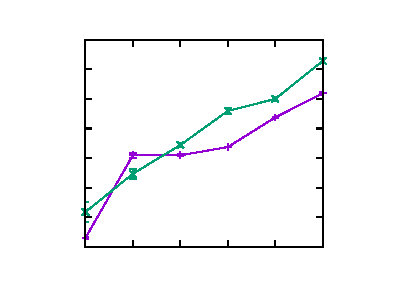
\includegraphics{sharedintbarrier}}%
    \gplfronttext
  \end{picture}%
\endgroup

		\caption{i5}
	\end{subfigure}
	\begin{subfigure}{0.5\textwidth}
		% GNUPLOT: LaTeX picture with Postscript
\begingroup
  \makeatletter
  \providecommand\color[2][]{%
    \GenericError{(gnuplot) \space\space\space\@spaces}{%
      Package color not loaded in conjunction with
      terminal option `colourtext'%
    }{See the gnuplot documentation for explanation.%
    }{Either use 'blacktext' in gnuplot or load the package
      color.sty in LaTeX.}%
    \renewcommand\color[2][]{}%
  }%
  \providecommand\includegraphics[2][]{%
    \GenericError{(gnuplot) \space\space\space\@spaces}{%
      Package graphicx or graphics not loaded%
    }{See the gnuplot documentation for explanation.%
    }{The gnuplot epslatex terminal needs graphicx.sty or graphics.sty.}%
    \renewcommand\includegraphics[2][]{}%
  }%
  \providecommand\rotatebox[2]{#2}%
  \@ifundefined{ifGPcolor}{%
    \newif\ifGPcolor
    \GPcolorfalse
  }{}%
  \@ifundefined{ifGPblacktext}{%
    \newif\ifGPblacktext
    \GPblacktexttrue
  }{}%
  % define a \g@addto@macro without @ in the name:
  \let\gplgaddtomacro\g@addto@macro
  % define empty templates for all commands taking text:
  \gdef\gplbacktext{}%
  \gdef\gplfronttext{}%
  \makeatother
  \ifGPblacktext
    % no textcolor at all
    \def\colorrgb#1{}%
    \def\colorgray#1{}%
  \else
    % gray or color?
    \ifGPcolor
      \def\colorrgb#1{\color[rgb]{#1}}%
      \def\colorgray#1{\color[gray]{#1}}%
      \expandafter\def\csname LTw\endcsname{\color{white}}%
      \expandafter\def\csname LTb\endcsname{\color{black}}%
      \expandafter\def\csname LTa\endcsname{\color{black}}%
      \expandafter\def\csname LT0\endcsname{\color[rgb]{1,0,0}}%
      \expandafter\def\csname LT1\endcsname{\color[rgb]{0,1,0}}%
      \expandafter\def\csname LT2\endcsname{\color[rgb]{0,0,1}}%
      \expandafter\def\csname LT3\endcsname{\color[rgb]{1,0,1}}%
      \expandafter\def\csname LT4\endcsname{\color[rgb]{0,1,1}}%
      \expandafter\def\csname LT5\endcsname{\color[rgb]{1,1,0}}%
      \expandafter\def\csname LT6\endcsname{\color[rgb]{0,0,0}}%
      \expandafter\def\csname LT7\endcsname{\color[rgb]{1,0.3,0}}%
      \expandafter\def\csname LT8\endcsname{\color[rgb]{0.5,0.5,0.5}}%
    \else
      % gray
      \def\colorrgb#1{\color{black}}%
      \def\colorgray#1{\color[gray]{#1}}%
      \expandafter\def\csname LTw\endcsname{\color{white}}%
      \expandafter\def\csname LTb\endcsname{\color{black}}%
      \expandafter\def\csname LTa\endcsname{\color{black}}%
      \expandafter\def\csname LT0\endcsname{\color{black}}%
      \expandafter\def\csname LT1\endcsname{\color{black}}%
      \expandafter\def\csname LT2\endcsname{\color{black}}%
      \expandafter\def\csname LT3\endcsname{\color{black}}%
      \expandafter\def\csname LT4\endcsname{\color{black}}%
      \expandafter\def\csname LT5\endcsname{\color{black}}%
      \expandafter\def\csname LT6\endcsname{\color{black}}%
      \expandafter\def\csname LT7\endcsname{\color{black}}%
      \expandafter\def\csname LT8\endcsname{\color{black}}%
    \fi
  \fi
    \setlength{\unitlength}{0.0500bp}%
    \ifx\gptboxheight\undefined%
      \newlength{\gptboxheight}%
      \newlength{\gptboxwidth}%
      \newsavebox{\gptboxtext}%
    \fi%
    \setlength{\fboxrule}{0.5pt}%
    \setlength{\fboxsep}{1pt}%
\begin{picture}(3600.00,2520.00)%
    \gplgaddtomacro\gplbacktext{%
      \csname LTb\endcsname%%
      \put(594,440){\makebox(0,0)[r]{\strut{}$0$}}%
      \put(594,812){\makebox(0,0)[r]{\strut{}$50$}}%
      \put(594,1184){\makebox(0,0)[r]{\strut{}$100$}}%
      \put(594,1556){\makebox(0,0)[r]{\strut{}$150$}}%
      \put(594,1928){\makebox(0,0)[r]{\strut{}$200$}}%
      \put(594,2300){\makebox(0,0)[r]{\strut{}$250$}}%
      \put(726,220){\makebox(0,0){\strut{}1}}%
      \put(891,220){\makebox(0,0){\strut{}2}}%
      \put(1221,220){\makebox(0,0){\strut{}4}}%
      \put(1882,220){\makebox(0,0){\strut{}8}}%
      \put(3203,220){\makebox(0,0){\strut{}16}}%
    }%
    \gplgaddtomacro\gplfronttext{%
    }%
    \gplbacktext
    \put(0,0){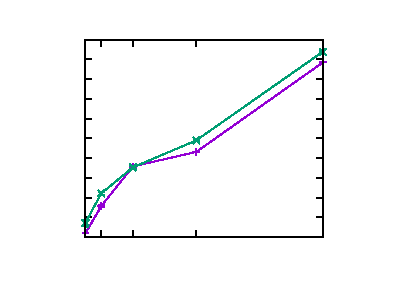
\includegraphics{sharedintbarrierdesktop}}%
    \gplfronttext
  \end{picture}%
\endgroup

		\caption{i7}
	\end{subfigure}
	\begin{subfigure}{1\textwidth}
		% GNUPLOT: LaTeX picture with Postscript
\begingroup
  \makeatletter
  \providecommand\color[2][]{%
    \GenericError{(gnuplot) \space\space\space\@spaces}{%
      Package color not loaded in conjunction with
      terminal option `colourtext'%
    }{See the gnuplot documentation for explanation.%
    }{Either use 'blacktext' in gnuplot or load the package
      color.sty in LaTeX.}%
    \renewcommand\color[2][]{}%
  }%
  \providecommand\includegraphics[2][]{%
    \GenericError{(gnuplot) \space\space\space\@spaces}{%
      Package graphicx or graphics not loaded%
    }{See the gnuplot documentation for explanation.%
    }{The gnuplot epslatex terminal needs graphicx.sty or graphics.sty.}%
    \renewcommand\includegraphics[2][]{}%
  }%
  \providecommand\rotatebox[2]{#2}%
  \@ifundefined{ifGPcolor}{%
    \newif\ifGPcolor
    \GPcolorfalse
  }{}%
  \@ifundefined{ifGPblacktext}{%
    \newif\ifGPblacktext
    \GPblacktexttrue
  }{}%
  % define a \g@addto@macro without @ in the name:
  \let\gplgaddtomacro\g@addto@macro
  % define empty templates for all commands taking text:
  \gdef\gplbacktext{}%
  \gdef\gplfronttext{}%
  \makeatother
  \ifGPblacktext
    % no textcolor at all
    \def\colorrgb#1{}%
    \def\colorgray#1{}%
  \else
    % gray or color?
    \ifGPcolor
      \def\colorrgb#1{\color[rgb]{#1}}%
      \def\colorgray#1{\color[gray]{#1}}%
      \expandafter\def\csname LTw\endcsname{\color{white}}%
      \expandafter\def\csname LTb\endcsname{\color{black}}%
      \expandafter\def\csname LTa\endcsname{\color{black}}%
      \expandafter\def\csname LT0\endcsname{\color[rgb]{1,0,0}}%
      \expandafter\def\csname LT1\endcsname{\color[rgb]{0,1,0}}%
      \expandafter\def\csname LT2\endcsname{\color[rgb]{0,0,1}}%
      \expandafter\def\csname LT3\endcsname{\color[rgb]{1,0,1}}%
      \expandafter\def\csname LT4\endcsname{\color[rgb]{0,1,1}}%
      \expandafter\def\csname LT5\endcsname{\color[rgb]{1,1,0}}%
      \expandafter\def\csname LT6\endcsname{\color[rgb]{0,0,0}}%
      \expandafter\def\csname LT7\endcsname{\color[rgb]{1,0.3,0}}%
      \expandafter\def\csname LT8\endcsname{\color[rgb]{0.5,0.5,0.5}}%
    \else
      % gray
      \def\colorrgb#1{\color{black}}%
      \def\colorgray#1{\color[gray]{#1}}%
      \expandafter\def\csname LTw\endcsname{\color{white}}%
      \expandafter\def\csname LTb\endcsname{\color{black}}%
      \expandafter\def\csname LTa\endcsname{\color{black}}%
      \expandafter\def\csname LT0\endcsname{\color{black}}%
      \expandafter\def\csname LT1\endcsname{\color{black}}%
      \expandafter\def\csname LT2\endcsname{\color{black}}%
      \expandafter\def\csname LT3\endcsname{\color{black}}%
      \expandafter\def\csname LT4\endcsname{\color{black}}%
      \expandafter\def\csname LT5\endcsname{\color{black}}%
      \expandafter\def\csname LT6\endcsname{\color{black}}%
      \expandafter\def\csname LT7\endcsname{\color{black}}%
      \expandafter\def\csname LT8\endcsname{\color{black}}%
    \fi
  \fi
    \setlength{\unitlength}{0.0500bp}%
    \ifx\gptboxheight\undefined%
      \newlength{\gptboxheight}%
      \newlength{\gptboxwidth}%
      \newsavebox{\gptboxtext}%
    \fi%
    \setlength{\fboxrule}{0.5pt}%
    \setlength{\fboxsep}{1pt}%
\begin{picture}(7200.00,2520.00)%
    \gplgaddtomacro\gplbacktext{%
      \csname LTb\endcsname%%
      \put(528,406){\makebox(0,0)[r]{\strut{}$0$}}%
      \put(528,643){\makebox(0,0)[r]{\strut{}$5\times10^{9}$}}%
      \put(528,880){\makebox(0,0)[r]{\strut{}$1\times10^{10}$}}%
      \put(528,1116){\makebox(0,0)[r]{\strut{}$1.5\times10^{10}$}}%
      \put(528,1353){\makebox(0,0)[r]{\strut{}$2\times10^{10}$}}%
      \put(528,1590){\makebox(0,0)[r]{\strut{}$2.5\times10^{10}$}}%
      \put(528,1827){\makebox(0,0)[r]{\strut{}$3\times10^{10}$}}%
      \put(528,2063){\makebox(0,0)[r]{\strut{}$3.5\times10^{10}$}}%
      \put(528,2300){\makebox(0,0)[r]{\strut{}$4\times10^{10}$}}%
      \put(660,274){\rotatebox{-45}{\makebox(0,0)[l]{\strut{}1}}}%
      \put(753,274){\rotatebox{-45}{\makebox(0,0)[l]{\strut{}2}}}%
      \put(940,274){\rotatebox{-45}{\makebox(0,0)[l]{\strut{}4}}}%
      \put(1313,274){\rotatebox{-45}{\makebox(0,0)[l]{\strut{}8}}}%
      \put(1686,274){\rotatebox{-45}{\makebox(0,0)[l]{\strut{}12}}}%
      \put(2060,274){\rotatebox{-45}{\makebox(0,0)[l]{\strut{}16}}}%
      \put(2806,274){\rotatebox{-45}{\makebox(0,0)[l]{\strut{}24}}}%
      \put(3553,274){\rotatebox{-45}{\makebox(0,0)[l]{\strut{}32}}}%
      \put(5046,274){\rotatebox{-45}{\makebox(0,0)[l]{\strut{}48}}}%
      \put(6539,274){\rotatebox{-45}{\makebox(0,0)[l]{\strut{}64}}}%
    }%
    \gplgaddtomacro\gplfronttext{%
    }%
    \gplbacktext
    \put(0,0){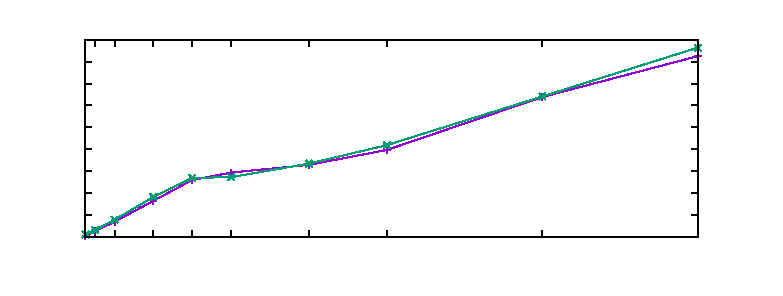
\includegraphics{sharedintbarrierserver}}%
    \gplfronttext
  \end{picture}%
\endgroup

		\caption{Xeon}
	\end{subfigure}
	\caption{Contended increments on \textbf{volatile} integers. The plots show
	nanoseconds per increment, as a function of the thread count.
	Please note that both axes vary across the plots.}
	\label{fig:cont}
\end{figure}

\begin{figure}[hbpt]
	\graphicspath{{plots/}}
	\begin{subfigure}{0.5\textwidth}
		% GNUPLOT: LaTeX picture with Postscript
\begingroup
  \makeatletter
  \providecommand\color[2][]{%
    \GenericError{(gnuplot) \space\space\space\@spaces}{%
      Package color not loaded in conjunction with
      terminal option `colourtext'%
    }{See the gnuplot documentation for explanation.%
    }{Either use 'blacktext' in gnuplot or load the package
      color.sty in LaTeX.}%
    \renewcommand\color[2][]{}%
  }%
  \providecommand\includegraphics[2][]{%
    \GenericError{(gnuplot) \space\space\space\@spaces}{%
      Package graphicx or graphics not loaded%
    }{See the gnuplot documentation for explanation.%
    }{The gnuplot epslatex terminal needs graphicx.sty or graphics.sty.}%
    \renewcommand\includegraphics[2][]{}%
  }%
  \providecommand\rotatebox[2]{#2}%
  \@ifundefined{ifGPcolor}{%
    \newif\ifGPcolor
    \GPcolorfalse
  }{}%
  \@ifundefined{ifGPblacktext}{%
    \newif\ifGPblacktext
    \GPblacktexttrue
  }{}%
  % define a \g@addto@macro without @ in the name:
  \let\gplgaddtomacro\g@addto@macro
  % define empty templates for all commands taking text:
  \gdef\gplbacktext{}%
  \gdef\gplfronttext{}%
  \makeatother
  \ifGPblacktext
    % no textcolor at all
    \def\colorrgb#1{}%
    \def\colorgray#1{}%
  \else
    % gray or color?
    \ifGPcolor
      \def\colorrgb#1{\color[rgb]{#1}}%
      \def\colorgray#1{\color[gray]{#1}}%
      \expandafter\def\csname LTw\endcsname{\color{white}}%
      \expandafter\def\csname LTb\endcsname{\color{black}}%
      \expandafter\def\csname LTa\endcsname{\color{black}}%
      \expandafter\def\csname LT0\endcsname{\color[rgb]{1,0,0}}%
      \expandafter\def\csname LT1\endcsname{\color[rgb]{0,1,0}}%
      \expandafter\def\csname LT2\endcsname{\color[rgb]{0,0,1}}%
      \expandafter\def\csname LT3\endcsname{\color[rgb]{1,0,1}}%
      \expandafter\def\csname LT4\endcsname{\color[rgb]{0,1,1}}%
      \expandafter\def\csname LT5\endcsname{\color[rgb]{1,1,0}}%
      \expandafter\def\csname LT6\endcsname{\color[rgb]{0,0,0}}%
      \expandafter\def\csname LT7\endcsname{\color[rgb]{1,0.3,0}}%
      \expandafter\def\csname LT8\endcsname{\color[rgb]{0.5,0.5,0.5}}%
    \else
      % gray
      \def\colorrgb#1{\color{black}}%
      \def\colorgray#1{\color[gray]{#1}}%
      \expandafter\def\csname LTw\endcsname{\color{white}}%
      \expandafter\def\csname LTb\endcsname{\color{black}}%
      \expandafter\def\csname LTa\endcsname{\color{black}}%
      \expandafter\def\csname LT0\endcsname{\color{black}}%
      \expandafter\def\csname LT1\endcsname{\color{black}}%
      \expandafter\def\csname LT2\endcsname{\color{black}}%
      \expandafter\def\csname LT3\endcsname{\color{black}}%
      \expandafter\def\csname LT4\endcsname{\color{black}}%
      \expandafter\def\csname LT5\endcsname{\color{black}}%
      \expandafter\def\csname LT6\endcsname{\color{black}}%
      \expandafter\def\csname LT7\endcsname{\color{black}}%
      \expandafter\def\csname LT8\endcsname{\color{black}}%
    \fi
  \fi
    \setlength{\unitlength}{0.0500bp}%
    \ifx\gptboxheight\undefined%
      \newlength{\gptboxheight}%
      \newlength{\gptboxwidth}%
      \newsavebox{\gptboxtext}%
    \fi%
    \setlength{\fboxrule}{0.5pt}%
    \setlength{\fboxsep}{1pt}%
\begin{picture}(3600.00,2520.00)%
    \gplgaddtomacro\gplbacktext{%
      \csname LTb\endcsname%%
      \put(594,440){\makebox(0,0)[r]{\strut{}$0$}}%
      \put(594,750){\makebox(0,0)[r]{\strut{}$0.5$}}%
      \put(594,1060){\makebox(0,0)[r]{\strut{}$1$}}%
      \put(594,1370){\makebox(0,0)[r]{\strut{}$1.5$}}%
      \put(594,1680){\makebox(0,0)[r]{\strut{}$2$}}%
      \put(594,1990){\makebox(0,0)[r]{\strut{}$2.5$}}%
      \put(594,2300){\makebox(0,0)[r]{\strut{}$3$}}%
      \put(726,220){\makebox(0,0){\strut{}1}}%
      \put(1221,220){\makebox(0,0){\strut{}2}}%
      \put(1717,220){\makebox(0,0){\strut{}3}}%
      \put(2212,220){\makebox(0,0){\strut{}4}}%
      \put(2708,220){\makebox(0,0){\strut{}5}}%
      \put(3203,220){\makebox(0,0){\strut{}6}}%
    }%
    \gplgaddtomacro\gplfronttext{%
    }%
    \gplbacktext
    \put(0,0){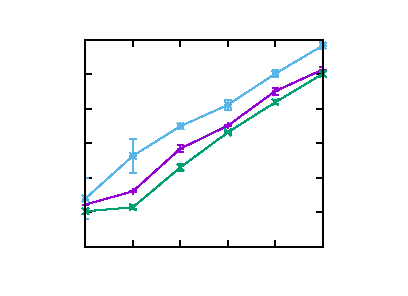
\includegraphics{sharedint}}%
    \gplfronttext
  \end{picture}%
\endgroup

		\caption{i5}
	\end{subfigure}
	\begin{subfigure}{0.5\textwidth}
		% GNUPLOT: LaTeX picture with Postscript
\begingroup
  \makeatletter
  \providecommand\color[2][]{%
    \GenericError{(gnuplot) \space\space\space\@spaces}{%
      Package color not loaded in conjunction with
      terminal option `colourtext'%
    }{See the gnuplot documentation for explanation.%
    }{Either use 'blacktext' in gnuplot or load the package
      color.sty in LaTeX.}%
    \renewcommand\color[2][]{}%
  }%
  \providecommand\includegraphics[2][]{%
    \GenericError{(gnuplot) \space\space\space\@spaces}{%
      Package graphicx or graphics not loaded%
    }{See the gnuplot documentation for explanation.%
    }{The gnuplot epslatex terminal needs graphicx.sty or graphics.sty.}%
    \renewcommand\includegraphics[2][]{}%
  }%
  \providecommand\rotatebox[2]{#2}%
  \@ifundefined{ifGPcolor}{%
    \newif\ifGPcolor
    \GPcolorfalse
  }{}%
  \@ifundefined{ifGPblacktext}{%
    \newif\ifGPblacktext
    \GPblacktexttrue
  }{}%
  % define a \g@addto@macro without @ in the name:
  \let\gplgaddtomacro\g@addto@macro
  % define empty templates for all commands taking text:
  \gdef\gplbacktext{}%
  \gdef\gplfronttext{}%
  \makeatother
  \ifGPblacktext
    % no textcolor at all
    \def\colorrgb#1{}%
    \def\colorgray#1{}%
  \else
    % gray or color?
    \ifGPcolor
      \def\colorrgb#1{\color[rgb]{#1}}%
      \def\colorgray#1{\color[gray]{#1}}%
      \expandafter\def\csname LTw\endcsname{\color{white}}%
      \expandafter\def\csname LTb\endcsname{\color{black}}%
      \expandafter\def\csname LTa\endcsname{\color{black}}%
      \expandafter\def\csname LT0\endcsname{\color[rgb]{1,0,0}}%
      \expandafter\def\csname LT1\endcsname{\color[rgb]{0,1,0}}%
      \expandafter\def\csname LT2\endcsname{\color[rgb]{0,0,1}}%
      \expandafter\def\csname LT3\endcsname{\color[rgb]{1,0,1}}%
      \expandafter\def\csname LT4\endcsname{\color[rgb]{0,1,1}}%
      \expandafter\def\csname LT5\endcsname{\color[rgb]{1,1,0}}%
      \expandafter\def\csname LT6\endcsname{\color[rgb]{0,0,0}}%
      \expandafter\def\csname LT7\endcsname{\color[rgb]{1,0.3,0}}%
      \expandafter\def\csname LT8\endcsname{\color[rgb]{0.5,0.5,0.5}}%
    \else
      % gray
      \def\colorrgb#1{\color{black}}%
      \def\colorgray#1{\color[gray]{#1}}%
      \expandafter\def\csname LTw\endcsname{\color{white}}%
      \expandafter\def\csname LTb\endcsname{\color{black}}%
      \expandafter\def\csname LTa\endcsname{\color{black}}%
      \expandafter\def\csname LT0\endcsname{\color{black}}%
      \expandafter\def\csname LT1\endcsname{\color{black}}%
      \expandafter\def\csname LT2\endcsname{\color{black}}%
      \expandafter\def\csname LT3\endcsname{\color{black}}%
      \expandafter\def\csname LT4\endcsname{\color{black}}%
      \expandafter\def\csname LT5\endcsname{\color{black}}%
      \expandafter\def\csname LT6\endcsname{\color{black}}%
      \expandafter\def\csname LT7\endcsname{\color{black}}%
      \expandafter\def\csname LT8\endcsname{\color{black}}%
    \fi
  \fi
    \setlength{\unitlength}{0.0500bp}%
    \ifx\gptboxheight\undefined%
      \newlength{\gptboxheight}%
      \newlength{\gptboxwidth}%
      \newsavebox{\gptboxtext}%
    \fi%
    \setlength{\fboxrule}{0.5pt}%
    \setlength{\fboxsep}{1pt}%
\begin{picture}(3600.00,2520.00)%
    \gplgaddtomacro\gplbacktext{%
      \csname LTb\endcsname%%
      \put(528,406){\makebox(0,0)[r]{\strut{}$0$}}%
      \put(528,785){\makebox(0,0)[r]{\strut{}$0.5$}}%
      \put(528,1164){\makebox(0,0)[r]{\strut{}$1$}}%
      \put(528,1542){\makebox(0,0)[r]{\strut{}$1.5$}}%
      \put(528,1921){\makebox(0,0)[r]{\strut{}$2$}}%
      \put(528,2300){\makebox(0,0)[r]{\strut{}$2.5$}}%
      \put(660,274){\rotatebox{-45}{\makebox(0,0)[l]{\strut{}1}}}%
      \put(812,274){\rotatebox{-45}{\makebox(0,0)[l]{\strut{}2}}}%
      \put(1116,274){\rotatebox{-45}{\makebox(0,0)[l]{\strut{}4}}}%
      \put(1724,274){\rotatebox{-45}{\makebox(0,0)[l]{\strut{}8}}}%
      \put(2939,274){\rotatebox{-45}{\makebox(0,0)[l]{\strut{}16}}}%
    }%
    \gplgaddtomacro\gplfronttext{%
    }%
    \gplbacktext
    \put(0,0){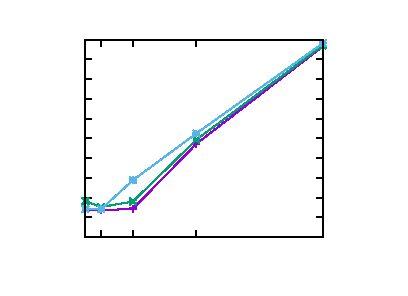
\includegraphics{sharedintdesktop}}%
    \gplfronttext
  \end{picture}%
\endgroup

		\caption{i7}
	\end{subfigure}
	\begin{subfigure}{1\textwidth}
		% GNUPLOT: LaTeX picture with Postscript
\begingroup
  \makeatletter
  \providecommand\color[2][]{%
    \GenericError{(gnuplot) \space\space\space\@spaces}{%
      Package color not loaded in conjunction with
      terminal option `colourtext'%
    }{See the gnuplot documentation for explanation.%
    }{Either use 'blacktext' in gnuplot or load the package
      color.sty in LaTeX.}%
    \renewcommand\color[2][]{}%
  }%
  \providecommand\includegraphics[2][]{%
    \GenericError{(gnuplot) \space\space\space\@spaces}{%
      Package graphicx or graphics not loaded%
    }{See the gnuplot documentation for explanation.%
    }{The gnuplot epslatex terminal needs graphicx.sty or graphics.sty.}%
    \renewcommand\includegraphics[2][]{}%
  }%
  \providecommand\rotatebox[2]{#2}%
  \@ifundefined{ifGPcolor}{%
    \newif\ifGPcolor
    \GPcolorfalse
  }{}%
  \@ifundefined{ifGPblacktext}{%
    \newif\ifGPblacktext
    \GPblacktexttrue
  }{}%
  % define a \g@addto@macro without @ in the name:
  \let\gplgaddtomacro\g@addto@macro
  % define empty templates for all commands taking text:
  \gdef\gplbacktext{}%
  \gdef\gplfronttext{}%
  \makeatother
  \ifGPblacktext
    % no textcolor at all
    \def\colorrgb#1{}%
    \def\colorgray#1{}%
  \else
    % gray or color?
    \ifGPcolor
      \def\colorrgb#1{\color[rgb]{#1}}%
      \def\colorgray#1{\color[gray]{#1}}%
      \expandafter\def\csname LTw\endcsname{\color{white}}%
      \expandafter\def\csname LTb\endcsname{\color{black}}%
      \expandafter\def\csname LTa\endcsname{\color{black}}%
      \expandafter\def\csname LT0\endcsname{\color[rgb]{1,0,0}}%
      \expandafter\def\csname LT1\endcsname{\color[rgb]{0,1,0}}%
      \expandafter\def\csname LT2\endcsname{\color[rgb]{0,0,1}}%
      \expandafter\def\csname LT3\endcsname{\color[rgb]{1,0,1}}%
      \expandafter\def\csname LT4\endcsname{\color[rgb]{0,1,1}}%
      \expandafter\def\csname LT5\endcsname{\color[rgb]{1,1,0}}%
      \expandafter\def\csname LT6\endcsname{\color[rgb]{0,0,0}}%
      \expandafter\def\csname LT7\endcsname{\color[rgb]{1,0.3,0}}%
      \expandafter\def\csname LT8\endcsname{\color[rgb]{0.5,0.5,0.5}}%
    \else
      % gray
      \def\colorrgb#1{\color{black}}%
      \def\colorgray#1{\color[gray]{#1}}%
      \expandafter\def\csname LTw\endcsname{\color{white}}%
      \expandafter\def\csname LTb\endcsname{\color{black}}%
      \expandafter\def\csname LTa\endcsname{\color{black}}%
      \expandafter\def\csname LT0\endcsname{\color{black}}%
      \expandafter\def\csname LT1\endcsname{\color{black}}%
      \expandafter\def\csname LT2\endcsname{\color{black}}%
      \expandafter\def\csname LT3\endcsname{\color{black}}%
      \expandafter\def\csname LT4\endcsname{\color{black}}%
      \expandafter\def\csname LT5\endcsname{\color{black}}%
      \expandafter\def\csname LT6\endcsname{\color{black}}%
      \expandafter\def\csname LT7\endcsname{\color{black}}%
      \expandafter\def\csname LT8\endcsname{\color{black}}%
    \fi
  \fi
    \setlength{\unitlength}{0.0500bp}%
    \ifx\gptboxheight\undefined%
      \newlength{\gptboxheight}%
      \newlength{\gptboxwidth}%
      \newsavebox{\gptboxtext}%
    \fi%
    \setlength{\fboxrule}{0.5pt}%
    \setlength{\fboxsep}{1pt}%
\begin{picture}(7200.00,2520.00)%
    \gplgaddtomacro\gplbacktext{%
      \csname LTb\endcsname%%
      \put(528,406){\makebox(0,0)[r]{\strut{}$0$}}%
      \put(528,643){\makebox(0,0)[r]{\strut{}$1\times10^{8}$}}%
      \put(528,880){\makebox(0,0)[r]{\strut{}$2\times10^{8}$}}%
      \put(528,1116){\makebox(0,0)[r]{\strut{}$3\times10^{8}$}}%
      \put(528,1353){\makebox(0,0)[r]{\strut{}$4\times10^{8}$}}%
      \put(528,1590){\makebox(0,0)[r]{\strut{}$5\times10^{8}$}}%
      \put(528,1827){\makebox(0,0)[r]{\strut{}$6\times10^{8}$}}%
      \put(528,2063){\makebox(0,0)[r]{\strut{}$7\times10^{8}$}}%
      \put(528,2300){\makebox(0,0)[r]{\strut{}$8\times10^{8}$}}%
      \put(660,274){\rotatebox{-45}{\makebox(0,0)[l]{\strut{}1}}}%
      \put(753,274){\rotatebox{-45}{\makebox(0,0)[l]{\strut{}2}}}%
      \put(940,274){\rotatebox{-45}{\makebox(0,0)[l]{\strut{}4}}}%
      \put(1313,274){\rotatebox{-45}{\makebox(0,0)[l]{\strut{}8}}}%
      \put(1686,274){\rotatebox{-45}{\makebox(0,0)[l]{\strut{}12}}}%
      \put(2060,274){\rotatebox{-45}{\makebox(0,0)[l]{\strut{}16}}}%
      \put(2806,274){\rotatebox{-45}{\makebox(0,0)[l]{\strut{}24}}}%
      \put(3553,274){\rotatebox{-45}{\makebox(0,0)[l]{\strut{}32}}}%
      \put(5046,274){\rotatebox{-45}{\makebox(0,0)[l]{\strut{}48}}}%
      \put(6539,274){\rotatebox{-45}{\makebox(0,0)[l]{\strut{}64}}}%
    }%
    \gplgaddtomacro\gplfronttext{%
    }%
    \gplbacktext
    \put(0,0){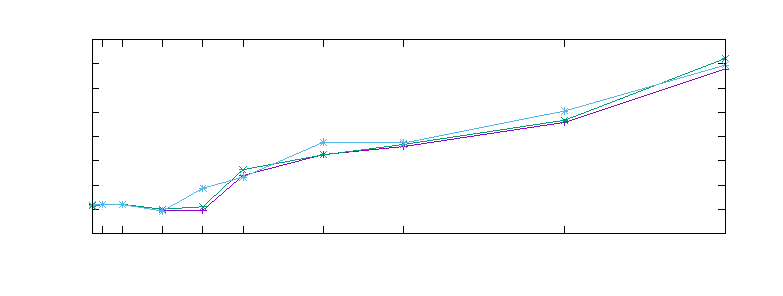
\includegraphics{sharedintserver}}%
    \gplfronttext
  \end{picture}%
\endgroup

		\caption{Xeon}
	\end{subfigure}
	\caption{Contended increments on \textbf{non-volatile} integers. The
	plots show nanoseconds per increment, as a function of the number of
	threads. Please note that both axes vary across the plots.}
	\label{fig:cont-nob}
\end{figure}

\mynote{include plots as ns-per-operation, concrete numbers/factors, and
discussion/conclusion on the results, concrete parameters: work not divided..}

\mynote{Konklusioner: Læsning er ikke gratis(!), pris for contended writes (både
med og uden barrier/volatile) siger en del om MESI pris (1 vs 2 tråde er
illustrativt), indikerer (løst) pris af at smide en cache-line frem og tilbage
mellem kerner}


\section{Practical applications}
While incrementing counters is useful, it is thankfully not the only thing we
build software for.
In this section we examine false sharing in 4 examples of more complicated
parallel programs.

First we will look at several programs that build histograms. These example
programs will motivate our approach from coarse- to fine-grained synchronization
with padding. One implementation also serves as an example of false sharing in
lock-free compare-and-swap based applications. We then use Quicksort as an example of the
divide and conquer paradigm, where the division of subproblems limit the need
for synchronization.
As examples of locking applications, we examine an implementation of k-means
clustering, as suggested in the January 2017 exam in Practical Concurrent and
Parallel Programming (PCPP) at the IT University of Copenhagen \cite{kmeansexam,
kmeansexamcode}, as well as two implementations of a concurrent hashmap data structure
used in the same course. Both of these applications are studied in
\cite{mystery}, and can be said to have instigated this project.

\subsection{Histogram builder}

Let us consider the problem of building a histogram: Given a sequence of
integers as input, we wish to build a data structure that maps numbers to their
frequencies in the input sequence.

A simple parallel algorithm for building a histogram presents itself: Divide the
sequence into a number of equal-sized sections, one for each thread. For each
element $a$ in its section, have each thread atomically increment a global
counter (or bucket) representing the frequency of $a$.

All the implementations we consider follow this basic formulation; they differ
only in how they ensure that the increment operations are atomic. We need to
ensure atomicity because the numbers in the input sequence may appear multiple
times, and in different segments, making it possible for more than a single
thread to increment the same frequency counter at the same time.

The histogram benchmarks are performed with the following parameters: An input
sequence which consists of 4 million randomly chosen integers $a\in[0,31]$, and
is divided evenly between threads. The more threads, the less work per thread.
We use 32 buckets: One for each possible number in the input. We will refer to
the number of buckets as the "width" of the histogram.

\subsubsection{Communication-free}
As a baseline for the multicore performance of the histogram problem, we examine
an implementation with minimal communication overhead. The strategy employed can
be thought of as a kind of avoidance: We arrange it so that part of the problem
can be solved in parallel, \textit{without ongoing communication between cores}.
After the parallel step, a single thread consolidates the thread-local
results produced by each thread. The only necessary communication or
synchronization is making the thread-local results visible to the thread that
executes the consolidation step, \textit{after} the parallel step is completed. Code snippet
\ref{code:histo-lockfree} outlines the implementation of this approach.

\begin{code}
\begin{Verbatim}[frame=single]
  List<Counter[]> perThreadCounts = ...;
  // Perform thread-local counts in parallel
  let taskCount parallel tasks do {
    // Thread-local counter array. A reference to the
    // same array is stored in perThreadCounts
    Counter[] counters = ...;
    final int from = ..., to = ...;
    for(int j = from; j < to; ++j) {
      counters[inputSequence[j]].value++;
    }
  }
  // Consolidate per-thread counts sequentially
  Counter[] globalCounts = new Counter[WIDTH];
  for(Counter[] localCounts : perThreadCounts) {
    for(int i = 0; i < WIDTH; ++i){
      globalCounts[i].value += localCounts[i].value;
    }
  }
\end{Verbatim}
	\caption{Simplified code for the communication-free version of the
	histogram builder.}
	\label{code:histo-lockfree}
\end{code}

\begin{figure}[hbtp]
	\centering
	\begin{tabular}{l r r}
		\hline
		\hline
		Platform & Time (ms) & SD (\%) \\
		\hline
		\input{plots/histo-local-lockfree}
		\hline
		\hline
	\end{tabular}
	\caption{Execution times for the communication-free histogram builder. Time
is the total wall-clock execution time, the standard deviation (SD) is given in
percent of the execution time.} \label{table:histo-lockfree}
\end{figure}

As we will see, this is by far the fastest of our solutions to the histogram. It
also scales relatively well with the number of cores.

\subsubsection{Coarse-grained locking}
When it comes to locking implementations, the simplest solution is for the
threads to take a single, shared lock anytime they increment a frequency
counter. This solution is slow. Only reading from the input sequence is
parallelised. At any time, only one thread can be incrementing a counter.

\begin{code}
\begin{Verbatim}[frame=single]
  Object lock = new Object();
  let taskCount parallel tasks do {
    final int from = ..., to = ...;
    for(int j = from; j < to; ++j) {
      synchronized(lock){
        counters[inputSequence[j]].value++;
      }
    }
  }
\end{Verbatim}
	\caption{Simplified code for the threads in the coarse-grained locking
	version of the histogram builder.}
\end{code}

The table in figure \ref{table:histo-global} shows the execution times of this
solution to the histogram problem. At we would expect, it scales poorly with the number of cores.

\begin{figure}[hbtp]
	\centering
	\begin{tabular}{l r r}
		\hline
		\hline
		Platform & Time (ms) & SD (\%) \\
		\hline
		\input{plots/histo-lock-global}
		\hline
		\hline
	\end{tabular}
	\caption{Execution times for the histogram builder using a single
global lock. Time is per input-element per thread, the standard deviation (SD)
is given in percentage of the execution time.}
	\label{table:histo-global}
\end{figure}

We will not measure it, but there is a possibility for false sharing in this
implementation. Consider the following sequence of operations, where we assume
counter0 and counter1 are in the same cache line:

\begin{enumerate}
	\item CPU0 updates counter 0. The cache line is left in CPU0's cache.
	\item \label{list:invalidation} CPU1 updates counter 1. The cache line is invalidated in CPU0's
		cache.
	\item \label{list:unneededread} CPU0 updates counter 0. The counter is not in CPU0's cache, and
		must be read from CPU1's cache instead.
\end{enumerate}

The cache miss in step \ref{list:unneededread} is unnecessary. It only occurs
because the two counters share a cache line, and because the other counter was
updated in step \ref{list:invalidation} by a different CPU core. The impact of
false sharing here is likely overshadowed by the poor choice of locking scheme.

There is another kind of unnecessary/false communication between CPU cores here,
that has nothing to do with sharing of cache lines: When a thread takes the
lock, updates from previous threads are guaranteed to be made visible to it.
Except for updates to the counter the thread is \textit{trying} to increment,
this is unnecessary.

\subsubsection{Fine-grained locking}
\label{sec:fine-grained-histo}
A better solution is to have different counters guarded by different locks. This
way, threads can perform all their work in parallel, except when different
threads work on counters guarded by the same lock. For practical applications
the ideal level of granularity should be determined by experiment. In this
experiment I use 32 locks: One lock for each bucket.

\begin{code}
\begin{Verbatim}[frame=single]
  Object[] locks = ...;
  let taskCount parallel tasks do {
    final int from = ..., to = ...;
    for(int j = from; j < to; ++j) {
      int a = inputSequence[j];
      synchronized(locks[a]){
        counters[a].value++;
      }
    }
  }
\end{Verbatim}
	\caption{Simplified code for the threads in the fine-grained locking
	version of the histogram builder.}
\end{code}

The improved level of parallelism increases the possibility for false sharing: In
the previous version only one thread could perform writes at a time. In this
version, threads holding different locks can in theory spend arbitrary amounts
of time invalidating each other's cache lines without doing any actual work.

There are two clear candidates for false sharing: The locks and the counters.
Neither are stored directly in the arrays: Locks must be object types, and are
hence stored as references, and the integers used for the counters are stored in
placeholder objects so we can declare them as \java{volatile}. False sharing of
the references stored in the arrays should therefore be irrelevant, but if the
objects are densely allocated, e.g. in a tight for-loop, they can still be
placed back-to-back in memory.

We measure the impact of false sharing by benchmarking versions with different
amounts of padding between the locks and counters.

\mynote{Because the elements/locks are objects, there is an additional,
unadvertised,  12 bytes of padding used for the counters, and something similar
for the locks (I can't say where in the object header the actual lock is, if it
is even in the object header). This should e noted somewhere, but probably not
here, as it goes for most of the benchmarks.}

\begin{figure}[hbtp]
	\centering
	\begin{tabular}{l r r r}
		\hline
		\hline
		Platform & Time wo. padding (ms) & Best time (ms) & Improvement \\
		\hline
		i5 & 113.0 & 100.88 & 10.7\% \\
		i7 & 71.88 & 59.9 & 16.9\% \\
		Xeon & 420.8 & 118.62 & 71.8\% \\
		\hline
		\hline
	\end{tabular}
	\caption{Best times vs. times without padding for the fine-grained
	histogram builder. Times are wall-clock execution times. Improvement is
	given in percent of the unpadded execution time: An improvement of
	71.8\% indicates that at least 71.8\% of the execution time is spend on
	unnecessary coherence communication in the unpadded version.}
	\label{table:hist-local}
\end{figure}

Figures \ref{fig:histo-local-i5}, \ref{fig:histo-local-i7}, and
\ref{fig:histo-local-xeon} show the wall-clock execution times using different
amounts of padding for the i5, i7, and Xeon platforms respectively. Each smaller
plot shows the execution time of the histogram builder, as a function of the
amount of padding between the counters. The third axis -- the amount of padding
between the locks -- is unrolled into different plots.

The table in figure \ref{table:hist-local} compares the unpadded times with the
best times for each platform.

The effect is smallest on the i5 platform: Using 128 bytes padding between
counters, and no padding between locks, yields a 10.7\% improvement on not using
padding. Padding the locks does not seem to benefit performance, and even makes
it worse in some cases.

On the i7 platform, padding locks and counters both benefits performance.
Padding 128 bytes between counters and 112 bytes between locks yields a 16.9\%
percent improvement on not using padding.

The most significant effect is seen on the Xeon platform. Like on the i7
platform, using padding is beneficial for both data structures, but here the
benefit from padding the locks is much more pronounced. Using 128 bytes of
padding for the counters and 112 bytes for the locks yields a 71.8\% improvement
on not using padding, indicating that most of the time is spent on cache
coherence overhead in the unpadded version.

There is a noteworthy caveat: The experiment runs with 48 threads on the Xeon
platform, but there are only 32 locks.
This cannot not be solved simply by increasing the
number of locks, as there are still only 32 distinct values in the input, and
therefore only 32 counters.
The scarcity of locks likely limits
throughput, but the false sharing impact should be the same without
this limitation, which is what we are concerned with.

It is not surprising that the platform with the most cores suffers the worst.
The more threads running in parallel, the bigger the likelihood of invalidating
a cache line that is relevant to another core. Furthermore, the invalidation
messages must be sent to all the other cores, and processors must wait for
acknowledgement messages from all the cores, so there is a lot more
communication occurring due the coherence protocol. The larger cache hierarchy
likely also means larger physical distances, which in turns makes communication
slower.

While our observations seem to agree with our understanding of false sharing,
two new mysteries present themselves: It is not clear why the execution time
keeps improving past 64-bytes padding, and it is not clear why padding the locks
has such a modest impact.

We would expect the performance to stop improving abruptly around 64
bytes, as that is the cache line size used by our hardware architectures.
One explanation for the continued improvements is the cache prefetch mechanism.
It is possible that the prefetch mechanism causes more than a single cache line
to be fetched. This is the explanation given for why the \java{@Contended}
annotation causes 128 bytes of padding to inserted on OpenJDK, under the
assumption that cache lines are half that size\cite{openjdkmailcontended}.
This explanation is in agreement with the Intel optimization
manual\cite{inteloptimize}, which states that the spatial prefetcher
"strives to complete every cache line fetched to the L2 cache with the pair line
that completes it to a 128-byte aligned chunk"\footnotemark. While this
prefetching does not incur a false sharing overhead, it will leave an additional
cache line in the CPU's cache. Another CPU might then later write to that
cache line, incurring unnecessary coherence overhead. The additional padding
does not prevent the prefetcher from loading the irrelevant cache line, but it
does prevent other threads from ever writing to it.

An explanation for the other mysterious artifact, the modest impact of padding
the locks, is more elusive. It seems to make sense that using a small number of
threads compared to the number of locks limits the impact of false sharing, as
it lessens the likelihood of threads working on the same cache lines. This
intuition fails to explain why the impact of padding the counters is larger: The
memory layout of the locks should be exactly the same as that of the counters,
and there are equally many of them.

\footnotetext{It is not entirely clear from the manual which microarchitectures
this applies to. It is stated for the Sandy Bridge microarchitecture, and seems
to apply to those that succeed it as well.}

\begin{figure}[hbpt]
	\graphicspath{{plots/}}
	\begin{subfigure}{0.32\textwidth}
		% GNUPLOT: LaTeX picture with Postscript
\begingroup
  \makeatletter
  \providecommand\color[2][]{%
    \GenericError{(gnuplot) \space\space\space\@spaces}{%
      Package color not loaded in conjunction with
      terminal option `colourtext'%
    }{See the gnuplot documentation for explanation.%
    }{Either use 'blacktext' in gnuplot or load the package
      color.sty in LaTeX.}%
    \renewcommand\color[2][]{}%
  }%
  \providecommand\includegraphics[2][]{%
    \GenericError{(gnuplot) \space\space\space\@spaces}{%
      Package graphicx or graphics not loaded%
    }{See the gnuplot documentation for explanation.%
    }{The gnuplot epslatex terminal needs graphicx.sty or graphics.sty.}%
    \renewcommand\includegraphics[2][]{}%
  }%
  \providecommand\rotatebox[2]{#2}%
  \@ifundefined{ifGPcolor}{%
    \newif\ifGPcolor
    \GPcolorfalse
  }{}%
  \@ifundefined{ifGPblacktext}{%
    \newif\ifGPblacktext
    \GPblacktexttrue
  }{}%
  % define a \g@addto@macro without @ in the name:
  \let\gplgaddtomacro\g@addto@macro
  % define empty templates for all commands taking text:
  \gdef\gplbacktext{}%
  \gdef\gplfronttext{}%
  \makeatother
  \ifGPblacktext
    % no textcolor at all
    \def\colorrgb#1{}%
    \def\colorgray#1{}%
  \else
    % gray or color?
    \ifGPcolor
      \def\colorrgb#1{\color[rgb]{#1}}%
      \def\colorgray#1{\color[gray]{#1}}%
      \expandafter\def\csname LTw\endcsname{\color{white}}%
      \expandafter\def\csname LTb\endcsname{\color{black}}%
      \expandafter\def\csname LTa\endcsname{\color{black}}%
      \expandafter\def\csname LT0\endcsname{\color[rgb]{1,0,0}}%
      \expandafter\def\csname LT1\endcsname{\color[rgb]{0,1,0}}%
      \expandafter\def\csname LT2\endcsname{\color[rgb]{0,0,1}}%
      \expandafter\def\csname LT3\endcsname{\color[rgb]{1,0,1}}%
      \expandafter\def\csname LT4\endcsname{\color[rgb]{0,1,1}}%
      \expandafter\def\csname LT5\endcsname{\color[rgb]{1,1,0}}%
      \expandafter\def\csname LT6\endcsname{\color[rgb]{0,0,0}}%
      \expandafter\def\csname LT7\endcsname{\color[rgb]{1,0.3,0}}%
      \expandafter\def\csname LT8\endcsname{\color[rgb]{0.5,0.5,0.5}}%
    \else
      % gray
      \def\colorrgb#1{\color{black}}%
      \def\colorgray#1{\color[gray]{#1}}%
      \expandafter\def\csname LTw\endcsname{\color{white}}%
      \expandafter\def\csname LTb\endcsname{\color{black}}%
      \expandafter\def\csname LTa\endcsname{\color{black}}%
      \expandafter\def\csname LT0\endcsname{\color{black}}%
      \expandafter\def\csname LT1\endcsname{\color{black}}%
      \expandafter\def\csname LT2\endcsname{\color{black}}%
      \expandafter\def\csname LT3\endcsname{\color{black}}%
      \expandafter\def\csname LT4\endcsname{\color{black}}%
      \expandafter\def\csname LT5\endcsname{\color{black}}%
      \expandafter\def\csname LT6\endcsname{\color{black}}%
      \expandafter\def\csname LT7\endcsname{\color{black}}%
      \expandafter\def\csname LT8\endcsname{\color{black}}%
    \fi
  \fi
    \setlength{\unitlength}{0.0500bp}%
    \ifx\gptboxheight\undefined%
      \newlength{\gptboxheight}%
      \newlength{\gptboxwidth}%
      \newsavebox{\gptboxtext}%
    \fi%
    \setlength{\fboxrule}{0.5pt}%
    \setlength{\fboxsep}{1pt}%
\begin{picture}(2880.00,2520.00)%
    \gplgaddtomacro\gplbacktext{%
      \csname LTb\endcsname%%
      \put(198,1100){\makebox(0,0)[r]{\strut{}}}%
      \put(198,1700){\makebox(0,0)[r]{\strut{}}}%
      \put(198,2300){\makebox(0,0)[r]{\strut{}}}%
      \put(330,368){\rotatebox{45}{\makebox(0,0)[r]{\strut{}$0$}}}%
      \put(868,368){\rotatebox{45}{\makebox(0,0)[r]{\strut{}$32$}}}%
      \put(1407,368){\rotatebox{45}{\makebox(0,0)[r]{\strut{}$64$}}}%
      \put(1945,368){\rotatebox{45}{\makebox(0,0)[r]{\strut{}$96$}}}%
      \put(2483,368){\rotatebox{45}{\makebox(0,0)[r]{\strut{}$128$}}}%
    }%
    \gplgaddtomacro\gplfronttext{%
    }%
    \gplbacktext
    \put(0,0){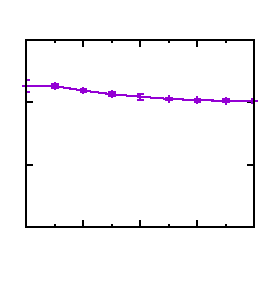
\includegraphics{Histo-lock-local-0-x1}}%
    \gplfronttext
  \end{picture}%
\endgroup

		\caption{0 bytes}
	\end{subfigure}
	\begin{subfigure}{0.32\textwidth}
		% GNUPLOT: LaTeX picture with Postscript
\begingroup
  \makeatletter
  \providecommand\color[2][]{%
    \GenericError{(gnuplot) \space\space\space\@spaces}{%
      Package color not loaded in conjunction with
      terminal option `colourtext'%
    }{See the gnuplot documentation for explanation.%
    }{Either use 'blacktext' in gnuplot or load the package
      color.sty in LaTeX.}%
    \renewcommand\color[2][]{}%
  }%
  \providecommand\includegraphics[2][]{%
    \GenericError{(gnuplot) \space\space\space\@spaces}{%
      Package graphicx or graphics not loaded%
    }{See the gnuplot documentation for explanation.%
    }{The gnuplot epslatex terminal needs graphicx.sty or graphics.sty.}%
    \renewcommand\includegraphics[2][]{}%
  }%
  \providecommand\rotatebox[2]{#2}%
  \@ifundefined{ifGPcolor}{%
    \newif\ifGPcolor
    \GPcolorfalse
  }{}%
  \@ifundefined{ifGPblacktext}{%
    \newif\ifGPblacktext
    \GPblacktexttrue
  }{}%
  % define a \g@addto@macro without @ in the name:
  \let\gplgaddtomacro\g@addto@macro
  % define empty templates for all commands taking text:
  \gdef\gplbacktext{}%
  \gdef\gplfronttext{}%
  \makeatother
  \ifGPblacktext
    % no textcolor at all
    \def\colorrgb#1{}%
    \def\colorgray#1{}%
  \else
    % gray or color?
    \ifGPcolor
      \def\colorrgb#1{\color[rgb]{#1}}%
      \def\colorgray#1{\color[gray]{#1}}%
      \expandafter\def\csname LTw\endcsname{\color{white}}%
      \expandafter\def\csname LTb\endcsname{\color{black}}%
      \expandafter\def\csname LTa\endcsname{\color{black}}%
      \expandafter\def\csname LT0\endcsname{\color[rgb]{1,0,0}}%
      \expandafter\def\csname LT1\endcsname{\color[rgb]{0,1,0}}%
      \expandafter\def\csname LT2\endcsname{\color[rgb]{0,0,1}}%
      \expandafter\def\csname LT3\endcsname{\color[rgb]{1,0,1}}%
      \expandafter\def\csname LT4\endcsname{\color[rgb]{0,1,1}}%
      \expandafter\def\csname LT5\endcsname{\color[rgb]{1,1,0}}%
      \expandafter\def\csname LT6\endcsname{\color[rgb]{0,0,0}}%
      \expandafter\def\csname LT7\endcsname{\color[rgb]{1,0.3,0}}%
      \expandafter\def\csname LT8\endcsname{\color[rgb]{0.5,0.5,0.5}}%
    \else
      % gray
      \def\colorrgb#1{\color{black}}%
      \def\colorgray#1{\color[gray]{#1}}%
      \expandafter\def\csname LTw\endcsname{\color{white}}%
      \expandafter\def\csname LTb\endcsname{\color{black}}%
      \expandafter\def\csname LTa\endcsname{\color{black}}%
      \expandafter\def\csname LT0\endcsname{\color{black}}%
      \expandafter\def\csname LT1\endcsname{\color{black}}%
      \expandafter\def\csname LT2\endcsname{\color{black}}%
      \expandafter\def\csname LT3\endcsname{\color{black}}%
      \expandafter\def\csname LT4\endcsname{\color{black}}%
      \expandafter\def\csname LT5\endcsname{\color{black}}%
      \expandafter\def\csname LT6\endcsname{\color{black}}%
      \expandafter\def\csname LT7\endcsname{\color{black}}%
      \expandafter\def\csname LT8\endcsname{\color{black}}%
    \fi
  \fi
    \setlength{\unitlength}{0.0500bp}%
    \ifx\gptboxheight\undefined%
      \newlength{\gptboxheight}%
      \newlength{\gptboxwidth}%
      \newsavebox{\gptboxtext}%
    \fi%
    \setlength{\fboxrule}{0.5pt}%
    \setlength{\fboxsep}{1pt}%
\begin{picture}(2376.00,2520.00)%
    \gplgaddtomacro\gplbacktext{%
      \csname LTb\endcsname%%
      \put(-40,1100){\makebox(0,0)[r]{\strut{}}}%
      \put(-40,1700){\makebox(0,0)[r]{\strut{}}}%
      \put(-40,2300){\makebox(0,0)[r]{\strut{}}}%
      \put(92,368){\rotatebox{45}{\makebox(0,0)[r]{\strut{}$0$}}}%
      \put(640,368){\rotatebox{45}{\makebox(0,0)[r]{\strut{}$32$}}}%
      \put(1188,368){\rotatebox{45}{\makebox(0,0)[r]{\strut{}$64$}}}%
      \put(1735,368){\rotatebox{45}{\makebox(0,0)[r]{\strut{}$96$}}}%
      \put(2283,368){\rotatebox{45}{\makebox(0,0)[r]{\strut{}$128$}}}%
    }%
    \gplgaddtomacro\gplfronttext{%
    }%
    \gplbacktext
    \put(0,0){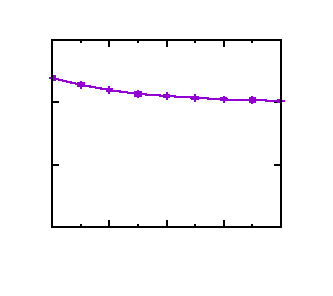
\includegraphics{Histo-lock-local-16-x1}}%
    \gplfronttext
  \end{picture}%
\endgroup

		\caption{16 bytes}
	\end{subfigure}
	\begin{subfigure}{0.32\textwidth}
		% GNUPLOT: LaTeX picture with Postscript
\begingroup
  \makeatletter
  \providecommand\color[2][]{%
    \GenericError{(gnuplot) \space\space\space\@spaces}{%
      Package color not loaded in conjunction with
      terminal option `colourtext'%
    }{See the gnuplot documentation for explanation.%
    }{Either use 'blacktext' in gnuplot or load the package
      color.sty in LaTeX.}%
    \renewcommand\color[2][]{}%
  }%
  \providecommand\includegraphics[2][]{%
    \GenericError{(gnuplot) \space\space\space\@spaces}{%
      Package graphicx or graphics not loaded%
    }{See the gnuplot documentation for explanation.%
    }{The gnuplot epslatex terminal needs graphicx.sty or graphics.sty.}%
    \renewcommand\includegraphics[2][]{}%
  }%
  \providecommand\rotatebox[2]{#2}%
  \@ifundefined{ifGPcolor}{%
    \newif\ifGPcolor
    \GPcolorfalse
  }{}%
  \@ifundefined{ifGPblacktext}{%
    \newif\ifGPblacktext
    \GPblacktexttrue
  }{}%
  % define a \g@addto@macro without @ in the name:
  \let\gplgaddtomacro\g@addto@macro
  % define empty templates for all commands taking text:
  \gdef\gplbacktext{}%
  \gdef\gplfronttext{}%
  \makeatother
  \ifGPblacktext
    % no textcolor at all
    \def\colorrgb#1{}%
    \def\colorgray#1{}%
  \else
    % gray or color?
    \ifGPcolor
      \def\colorrgb#1{\color[rgb]{#1}}%
      \def\colorgray#1{\color[gray]{#1}}%
      \expandafter\def\csname LTw\endcsname{\color{white}}%
      \expandafter\def\csname LTb\endcsname{\color{black}}%
      \expandafter\def\csname LTa\endcsname{\color{black}}%
      \expandafter\def\csname LT0\endcsname{\color[rgb]{1,0,0}}%
      \expandafter\def\csname LT1\endcsname{\color[rgb]{0,1,0}}%
      \expandafter\def\csname LT2\endcsname{\color[rgb]{0,0,1}}%
      \expandafter\def\csname LT3\endcsname{\color[rgb]{1,0,1}}%
      \expandafter\def\csname LT4\endcsname{\color[rgb]{0,1,1}}%
      \expandafter\def\csname LT5\endcsname{\color[rgb]{1,1,0}}%
      \expandafter\def\csname LT6\endcsname{\color[rgb]{0,0,0}}%
      \expandafter\def\csname LT7\endcsname{\color[rgb]{1,0.3,0}}%
      \expandafter\def\csname LT8\endcsname{\color[rgb]{0.5,0.5,0.5}}%
    \else
      % gray
      \def\colorrgb#1{\color{black}}%
      \def\colorgray#1{\color[gray]{#1}}%
      \expandafter\def\csname LTw\endcsname{\color{white}}%
      \expandafter\def\csname LTb\endcsname{\color{black}}%
      \expandafter\def\csname LTa\endcsname{\color{black}}%
      \expandafter\def\csname LT0\endcsname{\color{black}}%
      \expandafter\def\csname LT1\endcsname{\color{black}}%
      \expandafter\def\csname LT2\endcsname{\color{black}}%
      \expandafter\def\csname LT3\endcsname{\color{black}}%
      \expandafter\def\csname LT4\endcsname{\color{black}}%
      \expandafter\def\csname LT5\endcsname{\color{black}}%
      \expandafter\def\csname LT6\endcsname{\color{black}}%
      \expandafter\def\csname LT7\endcsname{\color{black}}%
      \expandafter\def\csname LT8\endcsname{\color{black}}%
    \fi
  \fi
    \setlength{\unitlength}{0.0500bp}%
    \ifx\gptboxheight\undefined%
      \newlength{\gptboxheight}%
      \newlength{\gptboxwidth}%
      \newsavebox{\gptboxtext}%
    \fi%
    \setlength{\fboxrule}{0.5pt}%
    \setlength{\fboxsep}{1pt}%
\begin{picture}(2376.00,2520.00)%
    \gplgaddtomacro\gplbacktext{%
      \csname LTb\endcsname%%
      \put(-40,1100){\makebox(0,0)[r]{\strut{}}}%
      \put(-40,1700){\makebox(0,0)[r]{\strut{}}}%
      \put(-40,2300){\makebox(0,0)[r]{\strut{}}}%
      \put(92,368){\rotatebox{45}{\makebox(0,0)[r]{\strut{}$0$}}}%
      \put(640,368){\rotatebox{45}{\makebox(0,0)[r]{\strut{}$32$}}}%
      \put(1188,368){\rotatebox{45}{\makebox(0,0)[r]{\strut{}$64$}}}%
      \put(1735,368){\rotatebox{45}{\makebox(0,0)[r]{\strut{}$96$}}}%
      \put(2283,368){\rotatebox{45}{\makebox(0,0)[r]{\strut{}$128$}}}%
    }%
    \gplgaddtomacro\gplfronttext{%
    }%
    \gplbacktext
    \put(0,0){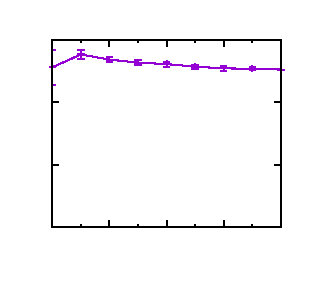
\includegraphics{Histo-lock-local-32-x1}}%
    \gplfronttext
  \end{picture}%
\endgroup

		\caption{32 bytes}
	\end{subfigure}
	\begin{subfigure}{0.32\textwidth}
		% GNUPLOT: LaTeX picture with Postscript
\begingroup
  \makeatletter
  \providecommand\color[2][]{%
    \GenericError{(gnuplot) \space\space\space\@spaces}{%
      Package color not loaded in conjunction with
      terminal option `colourtext'%
    }{See the gnuplot documentation for explanation.%
    }{Either use 'blacktext' in gnuplot or load the package
      color.sty in LaTeX.}%
    \renewcommand\color[2][]{}%
  }%
  \providecommand\includegraphics[2][]{%
    \GenericError{(gnuplot) \space\space\space\@spaces}{%
      Package graphicx or graphics not loaded%
    }{See the gnuplot documentation for explanation.%
    }{The gnuplot epslatex terminal needs graphicx.sty or graphics.sty.}%
    \renewcommand\includegraphics[2][]{}%
  }%
  \providecommand\rotatebox[2]{#2}%
  \@ifundefined{ifGPcolor}{%
    \newif\ifGPcolor
    \GPcolorfalse
  }{}%
  \@ifundefined{ifGPblacktext}{%
    \newif\ifGPblacktext
    \GPblacktexttrue
  }{}%
  % define a \g@addto@macro without @ in the name:
  \let\gplgaddtomacro\g@addto@macro
  % define empty templates for all commands taking text:
  \gdef\gplbacktext{}%
  \gdef\gplfronttext{}%
  \makeatother
  \ifGPblacktext
    % no textcolor at all
    \def\colorrgb#1{}%
    \def\colorgray#1{}%
  \else
    % gray or color?
    \ifGPcolor
      \def\colorrgb#1{\color[rgb]{#1}}%
      \def\colorgray#1{\color[gray]{#1}}%
      \expandafter\def\csname LTw\endcsname{\color{white}}%
      \expandafter\def\csname LTb\endcsname{\color{black}}%
      \expandafter\def\csname LTa\endcsname{\color{black}}%
      \expandafter\def\csname LT0\endcsname{\color[rgb]{1,0,0}}%
      \expandafter\def\csname LT1\endcsname{\color[rgb]{0,1,0}}%
      \expandafter\def\csname LT2\endcsname{\color[rgb]{0,0,1}}%
      \expandafter\def\csname LT3\endcsname{\color[rgb]{1,0,1}}%
      \expandafter\def\csname LT4\endcsname{\color[rgb]{0,1,1}}%
      \expandafter\def\csname LT5\endcsname{\color[rgb]{1,1,0}}%
      \expandafter\def\csname LT6\endcsname{\color[rgb]{0,0,0}}%
      \expandafter\def\csname LT7\endcsname{\color[rgb]{1,0.3,0}}%
      \expandafter\def\csname LT8\endcsname{\color[rgb]{0.5,0.5,0.5}}%
    \else
      % gray
      \def\colorrgb#1{\color{black}}%
      \def\colorgray#1{\color[gray]{#1}}%
      \expandafter\def\csname LTw\endcsname{\color{white}}%
      \expandafter\def\csname LTb\endcsname{\color{black}}%
      \expandafter\def\csname LTa\endcsname{\color{black}}%
      \expandafter\def\csname LT0\endcsname{\color{black}}%
      \expandafter\def\csname LT1\endcsname{\color{black}}%
      \expandafter\def\csname LT2\endcsname{\color{black}}%
      \expandafter\def\csname LT3\endcsname{\color{black}}%
      \expandafter\def\csname LT4\endcsname{\color{black}}%
      \expandafter\def\csname LT5\endcsname{\color{black}}%
      \expandafter\def\csname LT6\endcsname{\color{black}}%
      \expandafter\def\csname LT7\endcsname{\color{black}}%
      \expandafter\def\csname LT8\endcsname{\color{black}}%
    \fi
  \fi
    \setlength{\unitlength}{0.0500bp}%
    \ifx\gptboxheight\undefined%
      \newlength{\gptboxheight}%
      \newlength{\gptboxwidth}%
      \newsavebox{\gptboxtext}%
    \fi%
    \setlength{\fboxrule}{0.5pt}%
    \setlength{\fboxsep}{1pt}%
\begin{picture}(2880.00,2520.00)%
    \gplgaddtomacro\gplbacktext{%
      \csname LTb\endcsname%%
      \put(198,1100){\makebox(0,0)[r]{\strut{}}}%
      \put(198,1700){\makebox(0,0)[r]{\strut{}}}%
      \put(198,2300){\makebox(0,0)[r]{\strut{}}}%
      \put(330,368){\rotatebox{45}{\makebox(0,0)[r]{\strut{}$0$}}}%
      \put(868,368){\rotatebox{45}{\makebox(0,0)[r]{\strut{}$32$}}}%
      \put(1407,368){\rotatebox{45}{\makebox(0,0)[r]{\strut{}$64$}}}%
      \put(1945,368){\rotatebox{45}{\makebox(0,0)[r]{\strut{}$96$}}}%
      \put(2483,368){\rotatebox{45}{\makebox(0,0)[r]{\strut{}$128$}}}%
    }%
    \gplgaddtomacro\gplfronttext{%
    }%
    \gplbacktext
    \put(0,0){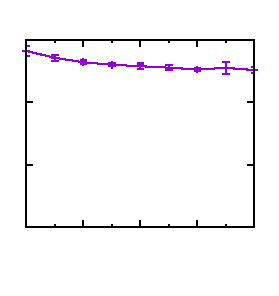
\includegraphics{Histo-lock-local-48-x1}}%
    \gplfronttext
  \end{picture}%
\endgroup

		\caption{48 bytes}
	\end{subfigure}
	\begin{subfigure}{0.32\textwidth}
		% GNUPLOT: LaTeX picture with Postscript
\begingroup
  \makeatletter
  \providecommand\color[2][]{%
    \GenericError{(gnuplot) \space\space\space\@spaces}{%
      Package color not loaded in conjunction with
      terminal option `colourtext'%
    }{See the gnuplot documentation for explanation.%
    }{Either use 'blacktext' in gnuplot or load the package
      color.sty in LaTeX.}%
    \renewcommand\color[2][]{}%
  }%
  \providecommand\includegraphics[2][]{%
    \GenericError{(gnuplot) \space\space\space\@spaces}{%
      Package graphicx or graphics not loaded%
    }{See the gnuplot documentation for explanation.%
    }{The gnuplot epslatex terminal needs graphicx.sty or graphics.sty.}%
    \renewcommand\includegraphics[2][]{}%
  }%
  \providecommand\rotatebox[2]{#2}%
  \@ifundefined{ifGPcolor}{%
    \newif\ifGPcolor
    \GPcolorfalse
  }{}%
  \@ifundefined{ifGPblacktext}{%
    \newif\ifGPblacktext
    \GPblacktexttrue
  }{}%
  % define a \g@addto@macro without @ in the name:
  \let\gplgaddtomacro\g@addto@macro
  % define empty templates for all commands taking text:
  \gdef\gplbacktext{}%
  \gdef\gplfronttext{}%
  \makeatother
  \ifGPblacktext
    % no textcolor at all
    \def\colorrgb#1{}%
    \def\colorgray#1{}%
  \else
    % gray or color?
    \ifGPcolor
      \def\colorrgb#1{\color[rgb]{#1}}%
      \def\colorgray#1{\color[gray]{#1}}%
      \expandafter\def\csname LTw\endcsname{\color{white}}%
      \expandafter\def\csname LTb\endcsname{\color{black}}%
      \expandafter\def\csname LTa\endcsname{\color{black}}%
      \expandafter\def\csname LT0\endcsname{\color[rgb]{1,0,0}}%
      \expandafter\def\csname LT1\endcsname{\color[rgb]{0,1,0}}%
      \expandafter\def\csname LT2\endcsname{\color[rgb]{0,0,1}}%
      \expandafter\def\csname LT3\endcsname{\color[rgb]{1,0,1}}%
      \expandafter\def\csname LT4\endcsname{\color[rgb]{0,1,1}}%
      \expandafter\def\csname LT5\endcsname{\color[rgb]{1,1,0}}%
      \expandafter\def\csname LT6\endcsname{\color[rgb]{0,0,0}}%
      \expandafter\def\csname LT7\endcsname{\color[rgb]{1,0.3,0}}%
      \expandafter\def\csname LT8\endcsname{\color[rgb]{0.5,0.5,0.5}}%
    \else
      % gray
      \def\colorrgb#1{\color{black}}%
      \def\colorgray#1{\color[gray]{#1}}%
      \expandafter\def\csname LTw\endcsname{\color{white}}%
      \expandafter\def\csname LTb\endcsname{\color{black}}%
      \expandafter\def\csname LTa\endcsname{\color{black}}%
      \expandafter\def\csname LT0\endcsname{\color{black}}%
      \expandafter\def\csname LT1\endcsname{\color{black}}%
      \expandafter\def\csname LT2\endcsname{\color{black}}%
      \expandafter\def\csname LT3\endcsname{\color{black}}%
      \expandafter\def\csname LT4\endcsname{\color{black}}%
      \expandafter\def\csname LT5\endcsname{\color{black}}%
      \expandafter\def\csname LT6\endcsname{\color{black}}%
      \expandafter\def\csname LT7\endcsname{\color{black}}%
      \expandafter\def\csname LT8\endcsname{\color{black}}%
    \fi
  \fi
    \setlength{\unitlength}{0.0500bp}%
    \ifx\gptboxheight\undefined%
      \newlength{\gptboxheight}%
      \newlength{\gptboxwidth}%
      \newsavebox{\gptboxtext}%
    \fi%
    \setlength{\fboxrule}{0.5pt}%
    \setlength{\fboxsep}{1pt}%
\begin{picture}(2376.00,2520.00)%
    \gplgaddtomacro\gplbacktext{%
      \csname LTb\endcsname%%
      \put(-40,1100){\makebox(0,0)[r]{\strut{}}}%
      \put(-40,1700){\makebox(0,0)[r]{\strut{}}}%
      \put(-40,2300){\makebox(0,0)[r]{\strut{}}}%
      \put(92,368){\rotatebox{45}{\makebox(0,0)[r]{\strut{}$0$}}}%
      \put(640,368){\rotatebox{45}{\makebox(0,0)[r]{\strut{}$32$}}}%
      \put(1188,368){\rotatebox{45}{\makebox(0,0)[r]{\strut{}$64$}}}%
      \put(1735,368){\rotatebox{45}{\makebox(0,0)[r]{\strut{}$96$}}}%
      \put(2283,368){\rotatebox{45}{\makebox(0,0)[r]{\strut{}$128$}}}%
    }%
    \gplgaddtomacro\gplfronttext{%
    }%
    \gplbacktext
    \put(0,0){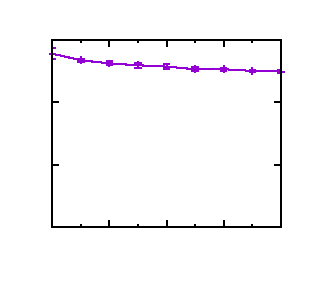
\includegraphics{Histo-lock-local-64-x1}}%
    \gplfronttext
  \end{picture}%
\endgroup

		\caption{64 bytes}
	\end{subfigure}
	\begin{subfigure}{0.32\textwidth}
		% GNUPLOT: LaTeX picture with Postscript
\begingroup
  \makeatletter
  \providecommand\color[2][]{%
    \GenericError{(gnuplot) \space\space\space\@spaces}{%
      Package color not loaded in conjunction with
      terminal option `colourtext'%
    }{See the gnuplot documentation for explanation.%
    }{Either use 'blacktext' in gnuplot or load the package
      color.sty in LaTeX.}%
    \renewcommand\color[2][]{}%
  }%
  \providecommand\includegraphics[2][]{%
    \GenericError{(gnuplot) \space\space\space\@spaces}{%
      Package graphicx or graphics not loaded%
    }{See the gnuplot documentation for explanation.%
    }{The gnuplot epslatex terminal needs graphicx.sty or graphics.sty.}%
    \renewcommand\includegraphics[2][]{}%
  }%
  \providecommand\rotatebox[2]{#2}%
  \@ifundefined{ifGPcolor}{%
    \newif\ifGPcolor
    \GPcolorfalse
  }{}%
  \@ifundefined{ifGPblacktext}{%
    \newif\ifGPblacktext
    \GPblacktexttrue
  }{}%
  % define a \g@addto@macro without @ in the name:
  \let\gplgaddtomacro\g@addto@macro
  % define empty templates for all commands taking text:
  \gdef\gplbacktext{}%
  \gdef\gplfronttext{}%
  \makeatother
  \ifGPblacktext
    % no textcolor at all
    \def\colorrgb#1{}%
    \def\colorgray#1{}%
  \else
    % gray or color?
    \ifGPcolor
      \def\colorrgb#1{\color[rgb]{#1}}%
      \def\colorgray#1{\color[gray]{#1}}%
      \expandafter\def\csname LTw\endcsname{\color{white}}%
      \expandafter\def\csname LTb\endcsname{\color{black}}%
      \expandafter\def\csname LTa\endcsname{\color{black}}%
      \expandafter\def\csname LT0\endcsname{\color[rgb]{1,0,0}}%
      \expandafter\def\csname LT1\endcsname{\color[rgb]{0,1,0}}%
      \expandafter\def\csname LT2\endcsname{\color[rgb]{0,0,1}}%
      \expandafter\def\csname LT3\endcsname{\color[rgb]{1,0,1}}%
      \expandafter\def\csname LT4\endcsname{\color[rgb]{0,1,1}}%
      \expandafter\def\csname LT5\endcsname{\color[rgb]{1,1,0}}%
      \expandafter\def\csname LT6\endcsname{\color[rgb]{0,0,0}}%
      \expandafter\def\csname LT7\endcsname{\color[rgb]{1,0.3,0}}%
      \expandafter\def\csname LT8\endcsname{\color[rgb]{0.5,0.5,0.5}}%
    \else
      % gray
      \def\colorrgb#1{\color{black}}%
      \def\colorgray#1{\color[gray]{#1}}%
      \expandafter\def\csname LTw\endcsname{\color{white}}%
      \expandafter\def\csname LTb\endcsname{\color{black}}%
      \expandafter\def\csname LTa\endcsname{\color{black}}%
      \expandafter\def\csname LT0\endcsname{\color{black}}%
      \expandafter\def\csname LT1\endcsname{\color{black}}%
      \expandafter\def\csname LT2\endcsname{\color{black}}%
      \expandafter\def\csname LT3\endcsname{\color{black}}%
      \expandafter\def\csname LT4\endcsname{\color{black}}%
      \expandafter\def\csname LT5\endcsname{\color{black}}%
      \expandafter\def\csname LT6\endcsname{\color{black}}%
      \expandafter\def\csname LT7\endcsname{\color{black}}%
      \expandafter\def\csname LT8\endcsname{\color{black}}%
    \fi
  \fi
    \setlength{\unitlength}{0.0500bp}%
    \ifx\gptboxheight\undefined%
      \newlength{\gptboxheight}%
      \newlength{\gptboxwidth}%
      \newsavebox{\gptboxtext}%
    \fi%
    \setlength{\fboxrule}{0.5pt}%
    \setlength{\fboxsep}{1pt}%
\begin{picture}(2880.00,2520.00)%
    \gplgaddtomacro\gplbacktext{%
      \csname LTb\endcsname%%
      \put(198,1100){\makebox(0,0)[r]{\strut{}}}%
      \put(198,1700){\makebox(0,0)[r]{\strut{}}}%
      \put(198,2300){\makebox(0,0)[r]{\strut{}}}%
      \put(330,368){\rotatebox{45}{\makebox(0,0)[r]{\strut{}$0$}}}%
      \put(868,368){\rotatebox{45}{\makebox(0,0)[r]{\strut{}$32$}}}%
      \put(1407,368){\rotatebox{45}{\makebox(0,0)[r]{\strut{}$64$}}}%
      \put(1945,368){\rotatebox{45}{\makebox(0,0)[r]{\strut{}$96$}}}%
      \put(2483,368){\rotatebox{45}{\makebox(0,0)[r]{\strut{}$128$}}}%
    }%
    \gplgaddtomacro\gplfronttext{%
    }%
    \gplbacktext
    \put(0,0){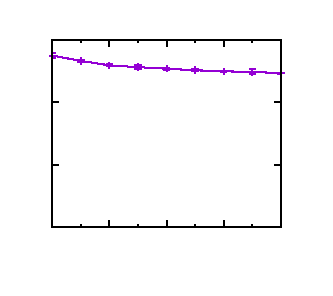
\includegraphics{Histo-lock-local-80-x1}}%
    \gplfronttext
  \end{picture}%
\endgroup

		\caption{80 bytes}
	\end{subfigure}
	\begin{subfigure}{0.32\textwidth}
		% GNUPLOT: LaTeX picture with Postscript
\begingroup
  \makeatletter
  \providecommand\color[2][]{%
    \GenericError{(gnuplot) \space\space\space\@spaces}{%
      Package color not loaded in conjunction with
      terminal option `colourtext'%
    }{See the gnuplot documentation for explanation.%
    }{Either use 'blacktext' in gnuplot or load the package
      color.sty in LaTeX.}%
    \renewcommand\color[2][]{}%
  }%
  \providecommand\includegraphics[2][]{%
    \GenericError{(gnuplot) \space\space\space\@spaces}{%
      Package graphicx or graphics not loaded%
    }{See the gnuplot documentation for explanation.%
    }{The gnuplot epslatex terminal needs graphicx.sty or graphics.sty.}%
    \renewcommand\includegraphics[2][]{}%
  }%
  \providecommand\rotatebox[2]{#2}%
  \@ifundefined{ifGPcolor}{%
    \newif\ifGPcolor
    \GPcolorfalse
  }{}%
  \@ifundefined{ifGPblacktext}{%
    \newif\ifGPblacktext
    \GPblacktexttrue
  }{}%
  % define a \g@addto@macro without @ in the name:
  \let\gplgaddtomacro\g@addto@macro
  % define empty templates for all commands taking text:
  \gdef\gplbacktext{}%
  \gdef\gplfronttext{}%
  \makeatother
  \ifGPblacktext
    % no textcolor at all
    \def\colorrgb#1{}%
    \def\colorgray#1{}%
  \else
    % gray or color?
    \ifGPcolor
      \def\colorrgb#1{\color[rgb]{#1}}%
      \def\colorgray#1{\color[gray]{#1}}%
      \expandafter\def\csname LTw\endcsname{\color{white}}%
      \expandafter\def\csname LTb\endcsname{\color{black}}%
      \expandafter\def\csname LTa\endcsname{\color{black}}%
      \expandafter\def\csname LT0\endcsname{\color[rgb]{1,0,0}}%
      \expandafter\def\csname LT1\endcsname{\color[rgb]{0,1,0}}%
      \expandafter\def\csname LT2\endcsname{\color[rgb]{0,0,1}}%
      \expandafter\def\csname LT3\endcsname{\color[rgb]{1,0,1}}%
      \expandafter\def\csname LT4\endcsname{\color[rgb]{0,1,1}}%
      \expandafter\def\csname LT5\endcsname{\color[rgb]{1,1,0}}%
      \expandafter\def\csname LT6\endcsname{\color[rgb]{0,0,0}}%
      \expandafter\def\csname LT7\endcsname{\color[rgb]{1,0.3,0}}%
      \expandafter\def\csname LT8\endcsname{\color[rgb]{0.5,0.5,0.5}}%
    \else
      % gray
      \def\colorrgb#1{\color{black}}%
      \def\colorgray#1{\color[gray]{#1}}%
      \expandafter\def\csname LTw\endcsname{\color{white}}%
      \expandafter\def\csname LTb\endcsname{\color{black}}%
      \expandafter\def\csname LTa\endcsname{\color{black}}%
      \expandafter\def\csname LT0\endcsname{\color{black}}%
      \expandafter\def\csname LT1\endcsname{\color{black}}%
      \expandafter\def\csname LT2\endcsname{\color{black}}%
      \expandafter\def\csname LT3\endcsname{\color{black}}%
      \expandafter\def\csname LT4\endcsname{\color{black}}%
      \expandafter\def\csname LT5\endcsname{\color{black}}%
      \expandafter\def\csname LT6\endcsname{\color{black}}%
      \expandafter\def\csname LT7\endcsname{\color{black}}%
      \expandafter\def\csname LT8\endcsname{\color{black}}%
    \fi
  \fi
    \setlength{\unitlength}{0.0500bp}%
    \ifx\gptboxheight\undefined%
      \newlength{\gptboxheight}%
      \newlength{\gptboxwidth}%
      \newsavebox{\gptboxtext}%
    \fi%
    \setlength{\fboxrule}{0.5pt}%
    \setlength{\fboxsep}{1pt}%
\begin{picture}(2880.00,2520.00)%
    \gplgaddtomacro\gplbacktext{%
      \csname LTb\endcsname%%
      \put(211,1100){\makebox(0,0)[r]{\strut{}}}%
      \put(211,1700){\makebox(0,0)[r]{\strut{}}}%
      \put(211,2300){\makebox(0,0)[r]{\strut{}}}%
      \put(343,368){\rotatebox{45}{\makebox(0,0)[r]{\strut{}$0$}}}%
      \put(891,368){\rotatebox{45}{\makebox(0,0)[r]{\strut{}$32$}}}%
      \put(1440,368){\rotatebox{45}{\makebox(0,0)[r]{\strut{}$64$}}}%
      \put(1988,368){\rotatebox{45}{\makebox(0,0)[r]{\strut{}$96$}}}%
      \put(2536,368){\rotatebox{45}{\makebox(0,0)[r]{\strut{}$128$}}}%
    }%
    \gplgaddtomacro\gplfronttext{%
    }%
    \gplbacktext
    \put(0,0){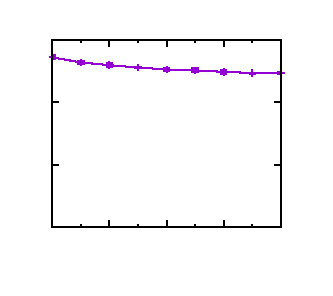
\includegraphics{Histo-lock-local-96-x1}}%
    \gplfronttext
  \end{picture}%
\endgroup

		\caption{96 bytes}
	\end{subfigure}
	\begin{subfigure}{0.32\textwidth}
		% GNUPLOT: LaTeX picture with Postscript
\begingroup
  \makeatletter
  \providecommand\color[2][]{%
    \GenericError{(gnuplot) \space\space\space\@spaces}{%
      Package color not loaded in conjunction with
      terminal option `colourtext'%
    }{See the gnuplot documentation for explanation.%
    }{Either use 'blacktext' in gnuplot or load the package
      color.sty in LaTeX.}%
    \renewcommand\color[2][]{}%
  }%
  \providecommand\includegraphics[2][]{%
    \GenericError{(gnuplot) \space\space\space\@spaces}{%
      Package graphicx or graphics not loaded%
    }{See the gnuplot documentation for explanation.%
    }{The gnuplot epslatex terminal needs graphicx.sty or graphics.sty.}%
    \renewcommand\includegraphics[2][]{}%
  }%
  \providecommand\rotatebox[2]{#2}%
  \@ifundefined{ifGPcolor}{%
    \newif\ifGPcolor
    \GPcolorfalse
  }{}%
  \@ifundefined{ifGPblacktext}{%
    \newif\ifGPblacktext
    \GPblacktexttrue
  }{}%
  % define a \g@addto@macro without @ in the name:
  \let\gplgaddtomacro\g@addto@macro
  % define empty templates for all commands taking text:
  \gdef\gplbacktext{}%
  \gdef\gplfronttext{}%
  \makeatother
  \ifGPblacktext
    % no textcolor at all
    \def\colorrgb#1{}%
    \def\colorgray#1{}%
  \else
    % gray or color?
    \ifGPcolor
      \def\colorrgb#1{\color[rgb]{#1}}%
      \def\colorgray#1{\color[gray]{#1}}%
      \expandafter\def\csname LTw\endcsname{\color{white}}%
      \expandafter\def\csname LTb\endcsname{\color{black}}%
      \expandafter\def\csname LTa\endcsname{\color{black}}%
      \expandafter\def\csname LT0\endcsname{\color[rgb]{1,0,0}}%
      \expandafter\def\csname LT1\endcsname{\color[rgb]{0,1,0}}%
      \expandafter\def\csname LT2\endcsname{\color[rgb]{0,0,1}}%
      \expandafter\def\csname LT3\endcsname{\color[rgb]{1,0,1}}%
      \expandafter\def\csname LT4\endcsname{\color[rgb]{0,1,1}}%
      \expandafter\def\csname LT5\endcsname{\color[rgb]{1,1,0}}%
      \expandafter\def\csname LT6\endcsname{\color[rgb]{0,0,0}}%
      \expandafter\def\csname LT7\endcsname{\color[rgb]{1,0.3,0}}%
      \expandafter\def\csname LT8\endcsname{\color[rgb]{0.5,0.5,0.5}}%
    \else
      % gray
      \def\colorrgb#1{\color{black}}%
      \def\colorgray#1{\color[gray]{#1}}%
      \expandafter\def\csname LTw\endcsname{\color{white}}%
      \expandafter\def\csname LTb\endcsname{\color{black}}%
      \expandafter\def\csname LTa\endcsname{\color{black}}%
      \expandafter\def\csname LT0\endcsname{\color{black}}%
      \expandafter\def\csname LT1\endcsname{\color{black}}%
      \expandafter\def\csname LT2\endcsname{\color{black}}%
      \expandafter\def\csname LT3\endcsname{\color{black}}%
      \expandafter\def\csname LT4\endcsname{\color{black}}%
      \expandafter\def\csname LT5\endcsname{\color{black}}%
      \expandafter\def\csname LT6\endcsname{\color{black}}%
      \expandafter\def\csname LT7\endcsname{\color{black}}%
      \expandafter\def\csname LT8\endcsname{\color{black}}%
    \fi
  \fi
    \setlength{\unitlength}{0.0500bp}%
    \ifx\gptboxheight\undefined%
      \newlength{\gptboxheight}%
      \newlength{\gptboxwidth}%
      \newsavebox{\gptboxtext}%
    \fi%
    \setlength{\fboxrule}{0.5pt}%
    \setlength{\fboxsep}{1pt}%
\begin{picture}(2376.00,2520.00)%
    \gplgaddtomacro\gplbacktext{%
      \csname LTb\endcsname%%
      \put(-40,1100){\makebox(0,0)[r]{\strut{}}}%
      \put(-40,1700){\makebox(0,0)[r]{\strut{}}}%
      \put(-40,2300){\makebox(0,0)[r]{\strut{}}}%
      \put(92,368){\rotatebox{45}{\makebox(0,0)[r]{\strut{}$0$}}}%
      \put(640,368){\rotatebox{45}{\makebox(0,0)[r]{\strut{}$32$}}}%
      \put(1188,368){\rotatebox{45}{\makebox(0,0)[r]{\strut{}$64$}}}%
      \put(1735,368){\rotatebox{45}{\makebox(0,0)[r]{\strut{}$96$}}}%
      \put(2283,368){\rotatebox{45}{\makebox(0,0)[r]{\strut{}$128$}}}%
    }%
    \gplgaddtomacro\gplfronttext{%
    }%
    \gplbacktext
    \put(0,0){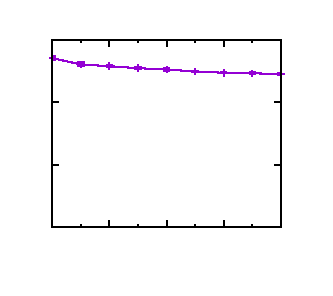
\includegraphics{Histo-lock-local-112-x1}}%
    \gplfronttext
  \end{picture}%
\endgroup

		\caption{112 bytes}
	\end{subfigure}
	\begin{subfigure}{0.32\textwidth}
		% GNUPLOT: LaTeX picture with Postscript
\begingroup
  \makeatletter
  \providecommand\color[2][]{%
    \GenericError{(gnuplot) \space\space\space\@spaces}{%
      Package color not loaded in conjunction with
      terminal option `colourtext'%
    }{See the gnuplot documentation for explanation.%
    }{Either use 'blacktext' in gnuplot or load the package
      color.sty in LaTeX.}%
    \renewcommand\color[2][]{}%
  }%
  \providecommand\includegraphics[2][]{%
    \GenericError{(gnuplot) \space\space\space\@spaces}{%
      Package graphicx or graphics not loaded%
    }{See the gnuplot documentation for explanation.%
    }{The gnuplot epslatex terminal needs graphicx.sty or graphics.sty.}%
    \renewcommand\includegraphics[2][]{}%
  }%
  \providecommand\rotatebox[2]{#2}%
  \@ifundefined{ifGPcolor}{%
    \newif\ifGPcolor
    \GPcolorfalse
  }{}%
  \@ifundefined{ifGPblacktext}{%
    \newif\ifGPblacktext
    \GPblacktexttrue
  }{}%
  % define a \g@addto@macro without @ in the name:
  \let\gplgaddtomacro\g@addto@macro
  % define empty templates for all commands taking text:
  \gdef\gplbacktext{}%
  \gdef\gplfronttext{}%
  \makeatother
  \ifGPblacktext
    % no textcolor at all
    \def\colorrgb#1{}%
    \def\colorgray#1{}%
  \else
    % gray or color?
    \ifGPcolor
      \def\colorrgb#1{\color[rgb]{#1}}%
      \def\colorgray#1{\color[gray]{#1}}%
      \expandafter\def\csname LTw\endcsname{\color{white}}%
      \expandafter\def\csname LTb\endcsname{\color{black}}%
      \expandafter\def\csname LTa\endcsname{\color{black}}%
      \expandafter\def\csname LT0\endcsname{\color[rgb]{1,0,0}}%
      \expandafter\def\csname LT1\endcsname{\color[rgb]{0,1,0}}%
      \expandafter\def\csname LT2\endcsname{\color[rgb]{0,0,1}}%
      \expandafter\def\csname LT3\endcsname{\color[rgb]{1,0,1}}%
      \expandafter\def\csname LT4\endcsname{\color[rgb]{0,1,1}}%
      \expandafter\def\csname LT5\endcsname{\color[rgb]{1,1,0}}%
      \expandafter\def\csname LT6\endcsname{\color[rgb]{0,0,0}}%
      \expandafter\def\csname LT7\endcsname{\color[rgb]{1,0.3,0}}%
      \expandafter\def\csname LT8\endcsname{\color[rgb]{0.5,0.5,0.5}}%
    \else
      % gray
      \def\colorrgb#1{\color{black}}%
      \def\colorgray#1{\color[gray]{#1}}%
      \expandafter\def\csname LTw\endcsname{\color{white}}%
      \expandafter\def\csname LTb\endcsname{\color{black}}%
      \expandafter\def\csname LTa\endcsname{\color{black}}%
      \expandafter\def\csname LT0\endcsname{\color{black}}%
      \expandafter\def\csname LT1\endcsname{\color{black}}%
      \expandafter\def\csname LT2\endcsname{\color{black}}%
      \expandafter\def\csname LT3\endcsname{\color{black}}%
      \expandafter\def\csname LT4\endcsname{\color{black}}%
      \expandafter\def\csname LT5\endcsname{\color{black}}%
      \expandafter\def\csname LT6\endcsname{\color{black}}%
      \expandafter\def\csname LT7\endcsname{\color{black}}%
      \expandafter\def\csname LT8\endcsname{\color{black}}%
    \fi
  \fi
    \setlength{\unitlength}{0.0500bp}%
    \ifx\gptboxheight\undefined%
      \newlength{\gptboxheight}%
      \newlength{\gptboxwidth}%
      \newsavebox{\gptboxtext}%
    \fi%
    \setlength{\fboxrule}{0.5pt}%
    \setlength{\fboxsep}{1pt}%
\begin{picture}(2880.00,2520.00)%
    \gplgaddtomacro\gplbacktext{%
      \csname LTb\endcsname%%
      \put(198,1100){\makebox(0,0)[r]{\strut{}}}%
      \put(198,1700){\makebox(0,0)[r]{\strut{}}}%
      \put(198,2300){\makebox(0,0)[r]{\strut{}}}%
      \put(330,368){\rotatebox{45}{\makebox(0,0)[r]{\strut{}$0$}}}%
      \put(868,368){\rotatebox{45}{\makebox(0,0)[r]{\strut{}$32$}}}%
      \put(1407,368){\rotatebox{45}{\makebox(0,0)[r]{\strut{}$64$}}}%
      \put(1945,368){\rotatebox{45}{\makebox(0,0)[r]{\strut{}$96$}}}%
      \put(2483,368){\rotatebox{45}{\makebox(0,0)[r]{\strut{}$128$}}}%
    }%
    \gplgaddtomacro\gplfronttext{%
    }%
    \gplbacktext
    \put(0,0){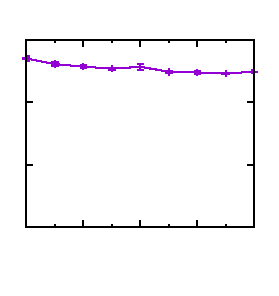
\includegraphics{Histo-lock-local-128-x1}}%
    \gplfronttext
  \end{picture}%
\endgroup

		\caption{128 bytes}
	\end{subfigure}
	\caption{The histogram problem on the i5 platform. Each plot uses a
	different amount of padding between the locks (specified beneath each
	plot). The plots show the running time of the histogram problem (each
	tick is 50 milliseconds. The axis starts at 0) as a function of the amount of padding between
	the histogram buckets in bytes.}
\end{figure}

\begin{figure}[hbpt]
	\graphicspath{{plots/}}
	\begin{subfigure}{0.32\textwidth}
		% GNUPLOT: LaTeX picture with Postscript
\begingroup
  \makeatletter
  \providecommand\color[2][]{%
    \GenericError{(gnuplot) \space\space\space\@spaces}{%
      Package color not loaded in conjunction with
      terminal option `colourtext'%
    }{See the gnuplot documentation for explanation.%
    }{Either use 'blacktext' in gnuplot or load the package
      color.sty in LaTeX.}%
    \renewcommand\color[2][]{}%
  }%
  \providecommand\includegraphics[2][]{%
    \GenericError{(gnuplot) \space\space\space\@spaces}{%
      Package graphicx or graphics not loaded%
    }{See the gnuplot documentation for explanation.%
    }{The gnuplot epslatex terminal needs graphicx.sty or graphics.sty.}%
    \renewcommand\includegraphics[2][]{}%
  }%
  \providecommand\rotatebox[2]{#2}%
  \@ifundefined{ifGPcolor}{%
    \newif\ifGPcolor
    \GPcolorfalse
  }{}%
  \@ifundefined{ifGPblacktext}{%
    \newif\ifGPblacktext
    \GPblacktexttrue
  }{}%
  % define a \g@addto@macro without @ in the name:
  \let\gplgaddtomacro\g@addto@macro
  % define empty templates for all commands taking text:
  \gdef\gplbacktext{}%
  \gdef\gplfronttext{}%
  \makeatother
  \ifGPblacktext
    % no textcolor at all
    \def\colorrgb#1{}%
    \def\colorgray#1{}%
  \else
    % gray or color?
    \ifGPcolor
      \def\colorrgb#1{\color[rgb]{#1}}%
      \def\colorgray#1{\color[gray]{#1}}%
      \expandafter\def\csname LTw\endcsname{\color{white}}%
      \expandafter\def\csname LTb\endcsname{\color{black}}%
      \expandafter\def\csname LTa\endcsname{\color{black}}%
      \expandafter\def\csname LT0\endcsname{\color[rgb]{1,0,0}}%
      \expandafter\def\csname LT1\endcsname{\color[rgb]{0,1,0}}%
      \expandafter\def\csname LT2\endcsname{\color[rgb]{0,0,1}}%
      \expandafter\def\csname LT3\endcsname{\color[rgb]{1,0,1}}%
      \expandafter\def\csname LT4\endcsname{\color[rgb]{0,1,1}}%
      \expandafter\def\csname LT5\endcsname{\color[rgb]{1,1,0}}%
      \expandafter\def\csname LT6\endcsname{\color[rgb]{0,0,0}}%
      \expandafter\def\csname LT7\endcsname{\color[rgb]{1,0.3,0}}%
      \expandafter\def\csname LT8\endcsname{\color[rgb]{0.5,0.5,0.5}}%
    \else
      % gray
      \def\colorrgb#1{\color{black}}%
      \def\colorgray#1{\color[gray]{#1}}%
      \expandafter\def\csname LTw\endcsname{\color{white}}%
      \expandafter\def\csname LTb\endcsname{\color{black}}%
      \expandafter\def\csname LTa\endcsname{\color{black}}%
      \expandafter\def\csname LT0\endcsname{\color{black}}%
      \expandafter\def\csname LT1\endcsname{\color{black}}%
      \expandafter\def\csname LT2\endcsname{\color{black}}%
      \expandafter\def\csname LT3\endcsname{\color{black}}%
      \expandafter\def\csname LT4\endcsname{\color{black}}%
      \expandafter\def\csname LT5\endcsname{\color{black}}%
      \expandafter\def\csname LT6\endcsname{\color{black}}%
      \expandafter\def\csname LT7\endcsname{\color{black}}%
      \expandafter\def\csname LT8\endcsname{\color{black}}%
    \fi
  \fi
    \setlength{\unitlength}{0.0500bp}%
    \ifx\gptboxheight\undefined%
      \newlength{\gptboxheight}%
      \newlength{\gptboxwidth}%
      \newsavebox{\gptboxtext}%
    \fi%
    \setlength{\fboxrule}{0.5pt}%
    \setlength{\fboxsep}{1pt}%
\begin{picture}(2880.00,2520.00)%
    \gplgaddtomacro\gplbacktext{%
      \csname LTb\endcsname%%
      \put(211,700){\makebox(0,0)[r]{\strut{}}}%
      \put(211,900){\makebox(0,0)[r]{\strut{}}}%
      \put(211,1100){\makebox(0,0)[r]{\strut{}}}%
      \put(211,1300){\makebox(0,0)[r]{\strut{}}}%
      \put(211,1500){\makebox(0,0)[r]{\strut{}}}%
      \put(211,1700){\makebox(0,0)[r]{\strut{}}}%
      \put(211,1900){\makebox(0,0)[r]{\strut{}}}%
      \put(211,2100){\makebox(0,0)[r]{\strut{}}}%
      \put(211,2300){\makebox(0,0)[r]{\strut{}}}%
      \put(343,368){\rotatebox{45}{\makebox(0,0)[r]{\strut{}$0$}}}%
      \put(891,368){\rotatebox{45}{\makebox(0,0)[r]{\strut{}$32$}}}%
      \put(1440,368){\rotatebox{45}{\makebox(0,0)[r]{\strut{}$64$}}}%
      \put(1988,368){\rotatebox{45}{\makebox(0,0)[r]{\strut{}$96$}}}%
      \put(2536,368){\rotatebox{45}{\makebox(0,0)[r]{\strut{}$128$}}}%
    }%
    \gplgaddtomacro\gplfronttext{%
    }%
    \gplbacktext
    \put(0,0){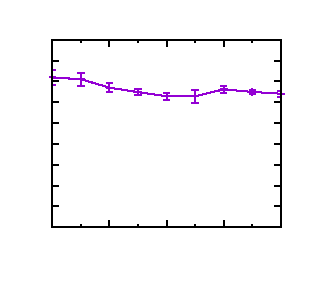
\includegraphics{Histo-lock-local-0-itu-desktop}}%
    \gplfronttext
  \end{picture}%
\endgroup

		\caption{0 bytes}
	\end{subfigure}
	\begin{subfigure}{0.32\textwidth}
		% GNUPLOT: LaTeX picture with Postscript
\begingroup
  \makeatletter
  \providecommand\color[2][]{%
    \GenericError{(gnuplot) \space\space\space\@spaces}{%
      Package color not loaded in conjunction with
      terminal option `colourtext'%
    }{See the gnuplot documentation for explanation.%
    }{Either use 'blacktext' in gnuplot or load the package
      color.sty in LaTeX.}%
    \renewcommand\color[2][]{}%
  }%
  \providecommand\includegraphics[2][]{%
    \GenericError{(gnuplot) \space\space\space\@spaces}{%
      Package graphicx or graphics not loaded%
    }{See the gnuplot documentation for explanation.%
    }{The gnuplot epslatex terminal needs graphicx.sty or graphics.sty.}%
    \renewcommand\includegraphics[2][]{}%
  }%
  \providecommand\rotatebox[2]{#2}%
  \@ifundefined{ifGPcolor}{%
    \newif\ifGPcolor
    \GPcolorfalse
  }{}%
  \@ifundefined{ifGPblacktext}{%
    \newif\ifGPblacktext
    \GPblacktexttrue
  }{}%
  % define a \g@addto@macro without @ in the name:
  \let\gplgaddtomacro\g@addto@macro
  % define empty templates for all commands taking text:
  \gdef\gplbacktext{}%
  \gdef\gplfronttext{}%
  \makeatother
  \ifGPblacktext
    % no textcolor at all
    \def\colorrgb#1{}%
    \def\colorgray#1{}%
  \else
    % gray or color?
    \ifGPcolor
      \def\colorrgb#1{\color[rgb]{#1}}%
      \def\colorgray#1{\color[gray]{#1}}%
      \expandafter\def\csname LTw\endcsname{\color{white}}%
      \expandafter\def\csname LTb\endcsname{\color{black}}%
      \expandafter\def\csname LTa\endcsname{\color{black}}%
      \expandafter\def\csname LT0\endcsname{\color[rgb]{1,0,0}}%
      \expandafter\def\csname LT1\endcsname{\color[rgb]{0,1,0}}%
      \expandafter\def\csname LT2\endcsname{\color[rgb]{0,0,1}}%
      \expandafter\def\csname LT3\endcsname{\color[rgb]{1,0,1}}%
      \expandafter\def\csname LT4\endcsname{\color[rgb]{0,1,1}}%
      \expandafter\def\csname LT5\endcsname{\color[rgb]{1,1,0}}%
      \expandafter\def\csname LT6\endcsname{\color[rgb]{0,0,0}}%
      \expandafter\def\csname LT7\endcsname{\color[rgb]{1,0.3,0}}%
      \expandafter\def\csname LT8\endcsname{\color[rgb]{0.5,0.5,0.5}}%
    \else
      % gray
      \def\colorrgb#1{\color{black}}%
      \def\colorgray#1{\color[gray]{#1}}%
      \expandafter\def\csname LTw\endcsname{\color{white}}%
      \expandafter\def\csname LTb\endcsname{\color{black}}%
      \expandafter\def\csname LTa\endcsname{\color{black}}%
      \expandafter\def\csname LT0\endcsname{\color{black}}%
      \expandafter\def\csname LT1\endcsname{\color{black}}%
      \expandafter\def\csname LT2\endcsname{\color{black}}%
      \expandafter\def\csname LT3\endcsname{\color{black}}%
      \expandafter\def\csname LT4\endcsname{\color{black}}%
      \expandafter\def\csname LT5\endcsname{\color{black}}%
      \expandafter\def\csname LT6\endcsname{\color{black}}%
      \expandafter\def\csname LT7\endcsname{\color{black}}%
      \expandafter\def\csname LT8\endcsname{\color{black}}%
    \fi
  \fi
    \setlength{\unitlength}{0.0500bp}%
    \ifx\gptboxheight\undefined%
      \newlength{\gptboxheight}%
      \newlength{\gptboxwidth}%
      \newsavebox{\gptboxtext}%
    \fi%
    \setlength{\fboxrule}{0.5pt}%
    \setlength{\fboxsep}{1pt}%
\begin{picture}(2880.00,2520.00)%
    \gplgaddtomacro\gplbacktext{%
      \csname LTb\endcsname%%
      \put(211,700){\makebox(0,0)[r]{\strut{}}}%
      \put(211,900){\makebox(0,0)[r]{\strut{}}}%
      \put(211,1100){\makebox(0,0)[r]{\strut{}}}%
      \put(211,1300){\makebox(0,0)[r]{\strut{}}}%
      \put(211,1500){\makebox(0,0)[r]{\strut{}}}%
      \put(211,1700){\makebox(0,0)[r]{\strut{}}}%
      \put(211,1900){\makebox(0,0)[r]{\strut{}}}%
      \put(211,2100){\makebox(0,0)[r]{\strut{}}}%
      \put(211,2300){\makebox(0,0)[r]{\strut{}}}%
      \put(343,368){\rotatebox{45}{\makebox(0,0)[r]{\strut{}$0$}}}%
      \put(891,368){\rotatebox{45}{\makebox(0,0)[r]{\strut{}$32$}}}%
      \put(1440,368){\rotatebox{45}{\makebox(0,0)[r]{\strut{}$64$}}}%
      \put(1988,368){\rotatebox{45}{\makebox(0,0)[r]{\strut{}$96$}}}%
      \put(2536,368){\rotatebox{45}{\makebox(0,0)[r]{\strut{}$128$}}}%
    }%
    \gplgaddtomacro\gplfronttext{%
    }%
    \gplbacktext
    \put(0,0){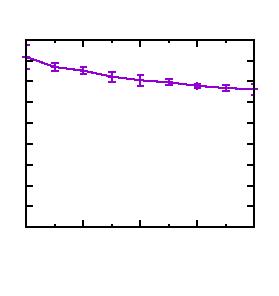
\includegraphics{Histo-lock-local-16-itu-desktop}}%
    \gplfronttext
  \end{picture}%
\endgroup

		\caption{16 bytes}
	\end{subfigure}
	\begin{subfigure}{0.32\textwidth}
		% GNUPLOT: LaTeX picture with Postscript
\begingroup
  \makeatletter
  \providecommand\color[2][]{%
    \GenericError{(gnuplot) \space\space\space\@spaces}{%
      Package color not loaded in conjunction with
      terminal option `colourtext'%
    }{See the gnuplot documentation for explanation.%
    }{Either use 'blacktext' in gnuplot or load the package
      color.sty in LaTeX.}%
    \renewcommand\color[2][]{}%
  }%
  \providecommand\includegraphics[2][]{%
    \GenericError{(gnuplot) \space\space\space\@spaces}{%
      Package graphicx or graphics not loaded%
    }{See the gnuplot documentation for explanation.%
    }{The gnuplot epslatex terminal needs graphicx.sty or graphics.sty.}%
    \renewcommand\includegraphics[2][]{}%
  }%
  \providecommand\rotatebox[2]{#2}%
  \@ifundefined{ifGPcolor}{%
    \newif\ifGPcolor
    \GPcolorfalse
  }{}%
  \@ifundefined{ifGPblacktext}{%
    \newif\ifGPblacktext
    \GPblacktexttrue
  }{}%
  % define a \g@addto@macro without @ in the name:
  \let\gplgaddtomacro\g@addto@macro
  % define empty templates for all commands taking text:
  \gdef\gplbacktext{}%
  \gdef\gplfronttext{}%
  \makeatother
  \ifGPblacktext
    % no textcolor at all
    \def\colorrgb#1{}%
    \def\colorgray#1{}%
  \else
    % gray or color?
    \ifGPcolor
      \def\colorrgb#1{\color[rgb]{#1}}%
      \def\colorgray#1{\color[gray]{#1}}%
      \expandafter\def\csname LTw\endcsname{\color{white}}%
      \expandafter\def\csname LTb\endcsname{\color{black}}%
      \expandafter\def\csname LTa\endcsname{\color{black}}%
      \expandafter\def\csname LT0\endcsname{\color[rgb]{1,0,0}}%
      \expandafter\def\csname LT1\endcsname{\color[rgb]{0,1,0}}%
      \expandafter\def\csname LT2\endcsname{\color[rgb]{0,0,1}}%
      \expandafter\def\csname LT3\endcsname{\color[rgb]{1,0,1}}%
      \expandafter\def\csname LT4\endcsname{\color[rgb]{0,1,1}}%
      \expandafter\def\csname LT5\endcsname{\color[rgb]{1,1,0}}%
      \expandafter\def\csname LT6\endcsname{\color[rgb]{0,0,0}}%
      \expandafter\def\csname LT7\endcsname{\color[rgb]{1,0.3,0}}%
      \expandafter\def\csname LT8\endcsname{\color[rgb]{0.5,0.5,0.5}}%
    \else
      % gray
      \def\colorrgb#1{\color{black}}%
      \def\colorgray#1{\color[gray]{#1}}%
      \expandafter\def\csname LTw\endcsname{\color{white}}%
      \expandafter\def\csname LTb\endcsname{\color{black}}%
      \expandafter\def\csname LTa\endcsname{\color{black}}%
      \expandafter\def\csname LT0\endcsname{\color{black}}%
      \expandafter\def\csname LT1\endcsname{\color{black}}%
      \expandafter\def\csname LT2\endcsname{\color{black}}%
      \expandafter\def\csname LT3\endcsname{\color{black}}%
      \expandafter\def\csname LT4\endcsname{\color{black}}%
      \expandafter\def\csname LT5\endcsname{\color{black}}%
      \expandafter\def\csname LT6\endcsname{\color{black}}%
      \expandafter\def\csname LT7\endcsname{\color{black}}%
      \expandafter\def\csname LT8\endcsname{\color{black}}%
    \fi
  \fi
    \setlength{\unitlength}{0.0500bp}%
    \ifx\gptboxheight\undefined%
      \newlength{\gptboxheight}%
      \newlength{\gptboxwidth}%
      \newsavebox{\gptboxtext}%
    \fi%
    \setlength{\fboxrule}{0.5pt}%
    \setlength{\fboxsep}{1pt}%
\begin{picture}(2376.00,2520.00)%
    \gplgaddtomacro\gplbacktext{%
      \csname LTb\endcsname%%
      \put(-40,700){\makebox(0,0)[r]{\strut{}}}%
      \put(-40,900){\makebox(0,0)[r]{\strut{}}}%
      \put(-40,1100){\makebox(0,0)[r]{\strut{}}}%
      \put(-40,1300){\makebox(0,0)[r]{\strut{}}}%
      \put(-40,1500){\makebox(0,0)[r]{\strut{}}}%
      \put(-40,1700){\makebox(0,0)[r]{\strut{}}}%
      \put(-40,1900){\makebox(0,0)[r]{\strut{}}}%
      \put(-40,2100){\makebox(0,0)[r]{\strut{}}}%
      \put(-40,2300){\makebox(0,0)[r]{\strut{}}}%
      \put(92,368){\rotatebox{45}{\makebox(0,0)[r]{\strut{}$0$}}}%
      \put(640,368){\rotatebox{45}{\makebox(0,0)[r]{\strut{}$32$}}}%
      \put(1188,368){\rotatebox{45}{\makebox(0,0)[r]{\strut{}$64$}}}%
      \put(1735,368){\rotatebox{45}{\makebox(0,0)[r]{\strut{}$96$}}}%
      \put(2283,368){\rotatebox{45}{\makebox(0,0)[r]{\strut{}$128$}}}%
    }%
    \gplgaddtomacro\gplfronttext{%
    }%
    \gplbacktext
    \put(0,0){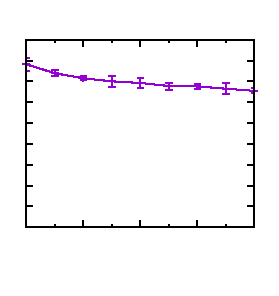
\includegraphics{Histo-lock-local-32-itu-desktop}}%
    \gplfronttext
  \end{picture}%
\endgroup

		\caption{32 bytes}
	\end{subfigure}
	\begin{subfigure}{0.32\textwidth}
		% GNUPLOT: LaTeX picture with Postscript
\begingroup
  \makeatletter
  \providecommand\color[2][]{%
    \GenericError{(gnuplot) \space\space\space\@spaces}{%
      Package color not loaded in conjunction with
      terminal option `colourtext'%
    }{See the gnuplot documentation for explanation.%
    }{Either use 'blacktext' in gnuplot or load the package
      color.sty in LaTeX.}%
    \renewcommand\color[2][]{}%
  }%
  \providecommand\includegraphics[2][]{%
    \GenericError{(gnuplot) \space\space\space\@spaces}{%
      Package graphicx or graphics not loaded%
    }{See the gnuplot documentation for explanation.%
    }{The gnuplot epslatex terminal needs graphicx.sty or graphics.sty.}%
    \renewcommand\includegraphics[2][]{}%
  }%
  \providecommand\rotatebox[2]{#2}%
  \@ifundefined{ifGPcolor}{%
    \newif\ifGPcolor
    \GPcolorfalse
  }{}%
  \@ifundefined{ifGPblacktext}{%
    \newif\ifGPblacktext
    \GPblacktexttrue
  }{}%
  % define a \g@addto@macro without @ in the name:
  \let\gplgaddtomacro\g@addto@macro
  % define empty templates for all commands taking text:
  \gdef\gplbacktext{}%
  \gdef\gplfronttext{}%
  \makeatother
  \ifGPblacktext
    % no textcolor at all
    \def\colorrgb#1{}%
    \def\colorgray#1{}%
  \else
    % gray or color?
    \ifGPcolor
      \def\colorrgb#1{\color[rgb]{#1}}%
      \def\colorgray#1{\color[gray]{#1}}%
      \expandafter\def\csname LTw\endcsname{\color{white}}%
      \expandafter\def\csname LTb\endcsname{\color{black}}%
      \expandafter\def\csname LTa\endcsname{\color{black}}%
      \expandafter\def\csname LT0\endcsname{\color[rgb]{1,0,0}}%
      \expandafter\def\csname LT1\endcsname{\color[rgb]{0,1,0}}%
      \expandafter\def\csname LT2\endcsname{\color[rgb]{0,0,1}}%
      \expandafter\def\csname LT3\endcsname{\color[rgb]{1,0,1}}%
      \expandafter\def\csname LT4\endcsname{\color[rgb]{0,1,1}}%
      \expandafter\def\csname LT5\endcsname{\color[rgb]{1,1,0}}%
      \expandafter\def\csname LT6\endcsname{\color[rgb]{0,0,0}}%
      \expandafter\def\csname LT7\endcsname{\color[rgb]{1,0.3,0}}%
      \expandafter\def\csname LT8\endcsname{\color[rgb]{0.5,0.5,0.5}}%
    \else
      % gray
      \def\colorrgb#1{\color{black}}%
      \def\colorgray#1{\color[gray]{#1}}%
      \expandafter\def\csname LTw\endcsname{\color{white}}%
      \expandafter\def\csname LTb\endcsname{\color{black}}%
      \expandafter\def\csname LTa\endcsname{\color{black}}%
      \expandafter\def\csname LT0\endcsname{\color{black}}%
      \expandafter\def\csname LT1\endcsname{\color{black}}%
      \expandafter\def\csname LT2\endcsname{\color{black}}%
      \expandafter\def\csname LT3\endcsname{\color{black}}%
      \expandafter\def\csname LT4\endcsname{\color{black}}%
      \expandafter\def\csname LT5\endcsname{\color{black}}%
      \expandafter\def\csname LT6\endcsname{\color{black}}%
      \expandafter\def\csname LT7\endcsname{\color{black}}%
      \expandafter\def\csname LT8\endcsname{\color{black}}%
    \fi
  \fi
    \setlength{\unitlength}{0.0500bp}%
    \ifx\gptboxheight\undefined%
      \newlength{\gptboxheight}%
      \newlength{\gptboxwidth}%
      \newsavebox{\gptboxtext}%
    \fi%
    \setlength{\fboxrule}{0.5pt}%
    \setlength{\fboxsep}{1pt}%
\begin{picture}(2880.00,2520.00)%
    \gplgaddtomacro\gplbacktext{%
      \csname LTb\endcsname%%
      \put(211,700){\makebox(0,0)[r]{\strut{}}}%
      \put(211,900){\makebox(0,0)[r]{\strut{}}}%
      \put(211,1100){\makebox(0,0)[r]{\strut{}}}%
      \put(211,1300){\makebox(0,0)[r]{\strut{}}}%
      \put(211,1500){\makebox(0,0)[r]{\strut{}}}%
      \put(211,1700){\makebox(0,0)[r]{\strut{}}}%
      \put(211,1900){\makebox(0,0)[r]{\strut{}}}%
      \put(211,2100){\makebox(0,0)[r]{\strut{}}}%
      \put(211,2300){\makebox(0,0)[r]{\strut{}}}%
      \put(343,368){\rotatebox{45}{\makebox(0,0)[r]{\strut{}$0$}}}%
      \put(891,368){\rotatebox{45}{\makebox(0,0)[r]{\strut{}$32$}}}%
      \put(1440,368){\rotatebox{45}{\makebox(0,0)[r]{\strut{}$64$}}}%
      \put(1988,368){\rotatebox{45}{\makebox(0,0)[r]{\strut{}$96$}}}%
      \put(2536,368){\rotatebox{45}{\makebox(0,0)[r]{\strut{}$128$}}}%
    }%
    \gplgaddtomacro\gplfronttext{%
    }%
    \gplbacktext
    \put(0,0){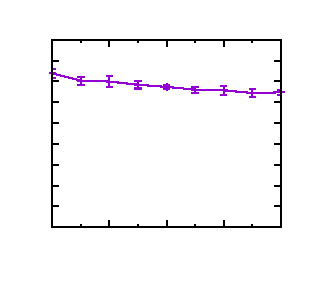
\includegraphics{Histo-lock-local-48-itu-desktop}}%
    \gplfronttext
  \end{picture}%
\endgroup

		\caption{48 bytes}
	\end{subfigure}
	\begin{subfigure}{0.32\textwidth}
		% GNUPLOT: LaTeX picture with Postscript
\begingroup
  \makeatletter
  \providecommand\color[2][]{%
    \GenericError{(gnuplot) \space\space\space\@spaces}{%
      Package color not loaded in conjunction with
      terminal option `colourtext'%
    }{See the gnuplot documentation for explanation.%
    }{Either use 'blacktext' in gnuplot or load the package
      color.sty in LaTeX.}%
    \renewcommand\color[2][]{}%
  }%
  \providecommand\includegraphics[2][]{%
    \GenericError{(gnuplot) \space\space\space\@spaces}{%
      Package graphicx or graphics not loaded%
    }{See the gnuplot documentation for explanation.%
    }{The gnuplot epslatex terminal needs graphicx.sty or graphics.sty.}%
    \renewcommand\includegraphics[2][]{}%
  }%
  \providecommand\rotatebox[2]{#2}%
  \@ifundefined{ifGPcolor}{%
    \newif\ifGPcolor
    \GPcolorfalse
  }{}%
  \@ifundefined{ifGPblacktext}{%
    \newif\ifGPblacktext
    \GPblacktexttrue
  }{}%
  % define a \g@addto@macro without @ in the name:
  \let\gplgaddtomacro\g@addto@macro
  % define empty templates for all commands taking text:
  \gdef\gplbacktext{}%
  \gdef\gplfronttext{}%
  \makeatother
  \ifGPblacktext
    % no textcolor at all
    \def\colorrgb#1{}%
    \def\colorgray#1{}%
  \else
    % gray or color?
    \ifGPcolor
      \def\colorrgb#1{\color[rgb]{#1}}%
      \def\colorgray#1{\color[gray]{#1}}%
      \expandafter\def\csname LTw\endcsname{\color{white}}%
      \expandafter\def\csname LTb\endcsname{\color{black}}%
      \expandafter\def\csname LTa\endcsname{\color{black}}%
      \expandafter\def\csname LT0\endcsname{\color[rgb]{1,0,0}}%
      \expandafter\def\csname LT1\endcsname{\color[rgb]{0,1,0}}%
      \expandafter\def\csname LT2\endcsname{\color[rgb]{0,0,1}}%
      \expandafter\def\csname LT3\endcsname{\color[rgb]{1,0,1}}%
      \expandafter\def\csname LT4\endcsname{\color[rgb]{0,1,1}}%
      \expandafter\def\csname LT5\endcsname{\color[rgb]{1,1,0}}%
      \expandafter\def\csname LT6\endcsname{\color[rgb]{0,0,0}}%
      \expandafter\def\csname LT7\endcsname{\color[rgb]{1,0.3,0}}%
      \expandafter\def\csname LT8\endcsname{\color[rgb]{0.5,0.5,0.5}}%
    \else
      % gray
      \def\colorrgb#1{\color{black}}%
      \def\colorgray#1{\color[gray]{#1}}%
      \expandafter\def\csname LTw\endcsname{\color{white}}%
      \expandafter\def\csname LTb\endcsname{\color{black}}%
      \expandafter\def\csname LTa\endcsname{\color{black}}%
      \expandafter\def\csname LT0\endcsname{\color{black}}%
      \expandafter\def\csname LT1\endcsname{\color{black}}%
      \expandafter\def\csname LT2\endcsname{\color{black}}%
      \expandafter\def\csname LT3\endcsname{\color{black}}%
      \expandafter\def\csname LT4\endcsname{\color{black}}%
      \expandafter\def\csname LT5\endcsname{\color{black}}%
      \expandafter\def\csname LT6\endcsname{\color{black}}%
      \expandafter\def\csname LT7\endcsname{\color{black}}%
      \expandafter\def\csname LT8\endcsname{\color{black}}%
    \fi
  \fi
    \setlength{\unitlength}{0.0500bp}%
    \ifx\gptboxheight\undefined%
      \newlength{\gptboxheight}%
      \newlength{\gptboxwidth}%
      \newsavebox{\gptboxtext}%
    \fi%
    \setlength{\fboxrule}{0.5pt}%
    \setlength{\fboxsep}{1pt}%
\begin{picture}(2880.00,2520.00)%
    \gplgaddtomacro\gplbacktext{%
      \csname LTb\endcsname%%
      \put(211,700){\makebox(0,0)[r]{\strut{}}}%
      \put(211,900){\makebox(0,0)[r]{\strut{}}}%
      \put(211,1100){\makebox(0,0)[r]{\strut{}}}%
      \put(211,1300){\makebox(0,0)[r]{\strut{}}}%
      \put(211,1500){\makebox(0,0)[r]{\strut{}}}%
      \put(211,1700){\makebox(0,0)[r]{\strut{}}}%
      \put(211,1900){\makebox(0,0)[r]{\strut{}}}%
      \put(211,2100){\makebox(0,0)[r]{\strut{}}}%
      \put(211,2300){\makebox(0,0)[r]{\strut{}}}%
      \put(343,368){\rotatebox{45}{\makebox(0,0)[r]{\strut{}$0$}}}%
      \put(891,368){\rotatebox{45}{\makebox(0,0)[r]{\strut{}$32$}}}%
      \put(1440,368){\rotatebox{45}{\makebox(0,0)[r]{\strut{}$64$}}}%
      \put(1988,368){\rotatebox{45}{\makebox(0,0)[r]{\strut{}$96$}}}%
      \put(2536,368){\rotatebox{45}{\makebox(0,0)[r]{\strut{}$128$}}}%
    }%
    \gplgaddtomacro\gplfronttext{%
    }%
    \gplbacktext
    \put(0,0){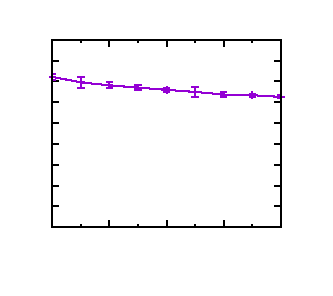
\includegraphics{Histo-lock-local-64-itu-desktop}}%
    \gplfronttext
  \end{picture}%
\endgroup

		\caption{64 bytes}
	\end{subfigure}
	\begin{subfigure}{0.32\textwidth}
		% GNUPLOT: LaTeX picture with Postscript
\begingroup
  \makeatletter
  \providecommand\color[2][]{%
    \GenericError{(gnuplot) \space\space\space\@spaces}{%
      Package color not loaded in conjunction with
      terminal option `colourtext'%
    }{See the gnuplot documentation for explanation.%
    }{Either use 'blacktext' in gnuplot or load the package
      color.sty in LaTeX.}%
    \renewcommand\color[2][]{}%
  }%
  \providecommand\includegraphics[2][]{%
    \GenericError{(gnuplot) \space\space\space\@spaces}{%
      Package graphicx or graphics not loaded%
    }{See the gnuplot documentation for explanation.%
    }{The gnuplot epslatex terminal needs graphicx.sty or graphics.sty.}%
    \renewcommand\includegraphics[2][]{}%
  }%
  \providecommand\rotatebox[2]{#2}%
  \@ifundefined{ifGPcolor}{%
    \newif\ifGPcolor
    \GPcolorfalse
  }{}%
  \@ifundefined{ifGPblacktext}{%
    \newif\ifGPblacktext
    \GPblacktexttrue
  }{}%
  % define a \g@addto@macro without @ in the name:
  \let\gplgaddtomacro\g@addto@macro
  % define empty templates for all commands taking text:
  \gdef\gplbacktext{}%
  \gdef\gplfronttext{}%
  \makeatother
  \ifGPblacktext
    % no textcolor at all
    \def\colorrgb#1{}%
    \def\colorgray#1{}%
  \else
    % gray or color?
    \ifGPcolor
      \def\colorrgb#1{\color[rgb]{#1}}%
      \def\colorgray#1{\color[gray]{#1}}%
      \expandafter\def\csname LTw\endcsname{\color{white}}%
      \expandafter\def\csname LTb\endcsname{\color{black}}%
      \expandafter\def\csname LTa\endcsname{\color{black}}%
      \expandafter\def\csname LT0\endcsname{\color[rgb]{1,0,0}}%
      \expandafter\def\csname LT1\endcsname{\color[rgb]{0,1,0}}%
      \expandafter\def\csname LT2\endcsname{\color[rgb]{0,0,1}}%
      \expandafter\def\csname LT3\endcsname{\color[rgb]{1,0,1}}%
      \expandafter\def\csname LT4\endcsname{\color[rgb]{0,1,1}}%
      \expandafter\def\csname LT5\endcsname{\color[rgb]{1,1,0}}%
      \expandafter\def\csname LT6\endcsname{\color[rgb]{0,0,0}}%
      \expandafter\def\csname LT7\endcsname{\color[rgb]{1,0.3,0}}%
      \expandafter\def\csname LT8\endcsname{\color[rgb]{0.5,0.5,0.5}}%
    \else
      % gray
      \def\colorrgb#1{\color{black}}%
      \def\colorgray#1{\color[gray]{#1}}%
      \expandafter\def\csname LTw\endcsname{\color{white}}%
      \expandafter\def\csname LTb\endcsname{\color{black}}%
      \expandafter\def\csname LTa\endcsname{\color{black}}%
      \expandafter\def\csname LT0\endcsname{\color{black}}%
      \expandafter\def\csname LT1\endcsname{\color{black}}%
      \expandafter\def\csname LT2\endcsname{\color{black}}%
      \expandafter\def\csname LT3\endcsname{\color{black}}%
      \expandafter\def\csname LT4\endcsname{\color{black}}%
      \expandafter\def\csname LT5\endcsname{\color{black}}%
      \expandafter\def\csname LT6\endcsname{\color{black}}%
      \expandafter\def\csname LT7\endcsname{\color{black}}%
      \expandafter\def\csname LT8\endcsname{\color{black}}%
    \fi
  \fi
    \setlength{\unitlength}{0.0500bp}%
    \ifx\gptboxheight\undefined%
      \newlength{\gptboxheight}%
      \newlength{\gptboxwidth}%
      \newsavebox{\gptboxtext}%
    \fi%
    \setlength{\fboxrule}{0.5pt}%
    \setlength{\fboxsep}{1pt}%
\begin{picture}(2880.00,2520.00)%
    \gplgaddtomacro\gplbacktext{%
      \csname LTb\endcsname%%
      \put(211,700){\makebox(0,0)[r]{\strut{}}}%
      \put(211,900){\makebox(0,0)[r]{\strut{}}}%
      \put(211,1100){\makebox(0,0)[r]{\strut{}}}%
      \put(211,1300){\makebox(0,0)[r]{\strut{}}}%
      \put(211,1500){\makebox(0,0)[r]{\strut{}}}%
      \put(211,1700){\makebox(0,0)[r]{\strut{}}}%
      \put(211,1900){\makebox(0,0)[r]{\strut{}}}%
      \put(211,2100){\makebox(0,0)[r]{\strut{}}}%
      \put(211,2300){\makebox(0,0)[r]{\strut{}}}%
      \put(343,368){\rotatebox{45}{\makebox(0,0)[r]{\strut{}$0$}}}%
      \put(891,368){\rotatebox{45}{\makebox(0,0)[r]{\strut{}$32$}}}%
      \put(1440,368){\rotatebox{45}{\makebox(0,0)[r]{\strut{}$64$}}}%
      \put(1988,368){\rotatebox{45}{\makebox(0,0)[r]{\strut{}$96$}}}%
      \put(2536,368){\rotatebox{45}{\makebox(0,0)[r]{\strut{}$128$}}}%
    }%
    \gplgaddtomacro\gplfronttext{%
    }%
    \gplbacktext
    \put(0,0){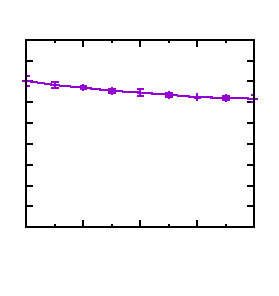
\includegraphics{Histo-lock-local-80-itu-desktop}}%
    \gplfronttext
  \end{picture}%
\endgroup

		\caption{80 bytes}
	\end{subfigure}
	\begin{subfigure}{0.32\textwidth}
		% GNUPLOT: LaTeX picture with Postscript
\begingroup
  \makeatletter
  \providecommand\color[2][]{%
    \GenericError{(gnuplot) \space\space\space\@spaces}{%
      Package color not loaded in conjunction with
      terminal option `colourtext'%
    }{See the gnuplot documentation for explanation.%
    }{Either use 'blacktext' in gnuplot or load the package
      color.sty in LaTeX.}%
    \renewcommand\color[2][]{}%
  }%
  \providecommand\includegraphics[2][]{%
    \GenericError{(gnuplot) \space\space\space\@spaces}{%
      Package graphicx or graphics not loaded%
    }{See the gnuplot documentation for explanation.%
    }{The gnuplot epslatex terminal needs graphicx.sty or graphics.sty.}%
    \renewcommand\includegraphics[2][]{}%
  }%
  \providecommand\rotatebox[2]{#2}%
  \@ifundefined{ifGPcolor}{%
    \newif\ifGPcolor
    \GPcolorfalse
  }{}%
  \@ifundefined{ifGPblacktext}{%
    \newif\ifGPblacktext
    \GPblacktexttrue
  }{}%
  % define a \g@addto@macro without @ in the name:
  \let\gplgaddtomacro\g@addto@macro
  % define empty templates for all commands taking text:
  \gdef\gplbacktext{}%
  \gdef\gplfronttext{}%
  \makeatother
  \ifGPblacktext
    % no textcolor at all
    \def\colorrgb#1{}%
    \def\colorgray#1{}%
  \else
    % gray or color?
    \ifGPcolor
      \def\colorrgb#1{\color[rgb]{#1}}%
      \def\colorgray#1{\color[gray]{#1}}%
      \expandafter\def\csname LTw\endcsname{\color{white}}%
      \expandafter\def\csname LTb\endcsname{\color{black}}%
      \expandafter\def\csname LTa\endcsname{\color{black}}%
      \expandafter\def\csname LT0\endcsname{\color[rgb]{1,0,0}}%
      \expandafter\def\csname LT1\endcsname{\color[rgb]{0,1,0}}%
      \expandafter\def\csname LT2\endcsname{\color[rgb]{0,0,1}}%
      \expandafter\def\csname LT3\endcsname{\color[rgb]{1,0,1}}%
      \expandafter\def\csname LT4\endcsname{\color[rgb]{0,1,1}}%
      \expandafter\def\csname LT5\endcsname{\color[rgb]{1,1,0}}%
      \expandafter\def\csname LT6\endcsname{\color[rgb]{0,0,0}}%
      \expandafter\def\csname LT7\endcsname{\color[rgb]{1,0.3,0}}%
      \expandafter\def\csname LT8\endcsname{\color[rgb]{0.5,0.5,0.5}}%
    \else
      % gray
      \def\colorrgb#1{\color{black}}%
      \def\colorgray#1{\color[gray]{#1}}%
      \expandafter\def\csname LTw\endcsname{\color{white}}%
      \expandafter\def\csname LTb\endcsname{\color{black}}%
      \expandafter\def\csname LTa\endcsname{\color{black}}%
      \expandafter\def\csname LT0\endcsname{\color{black}}%
      \expandafter\def\csname LT1\endcsname{\color{black}}%
      \expandafter\def\csname LT2\endcsname{\color{black}}%
      \expandafter\def\csname LT3\endcsname{\color{black}}%
      \expandafter\def\csname LT4\endcsname{\color{black}}%
      \expandafter\def\csname LT5\endcsname{\color{black}}%
      \expandafter\def\csname LT6\endcsname{\color{black}}%
      \expandafter\def\csname LT7\endcsname{\color{black}}%
      \expandafter\def\csname LT8\endcsname{\color{black}}%
    \fi
  \fi
    \setlength{\unitlength}{0.0500bp}%
    \ifx\gptboxheight\undefined%
      \newlength{\gptboxheight}%
      \newlength{\gptboxwidth}%
      \newsavebox{\gptboxtext}%
    \fi%
    \setlength{\fboxrule}{0.5pt}%
    \setlength{\fboxsep}{1pt}%
\begin{picture}(2376.00,2520.00)%
    \gplgaddtomacro\gplbacktext{%
      \csname LTb\endcsname%%
      \put(-40,700){\makebox(0,0)[r]{\strut{}}}%
      \put(-40,900){\makebox(0,0)[r]{\strut{}}}%
      \put(-40,1100){\makebox(0,0)[r]{\strut{}}}%
      \put(-40,1300){\makebox(0,0)[r]{\strut{}}}%
      \put(-40,1500){\makebox(0,0)[r]{\strut{}}}%
      \put(-40,1700){\makebox(0,0)[r]{\strut{}}}%
      \put(-40,1900){\makebox(0,0)[r]{\strut{}}}%
      \put(-40,2100){\makebox(0,0)[r]{\strut{}}}%
      \put(-40,2300){\makebox(0,0)[r]{\strut{}}}%
      \put(92,368){\rotatebox{45}{\makebox(0,0)[r]{\strut{}$0$}}}%
      \put(640,368){\rotatebox{45}{\makebox(0,0)[r]{\strut{}$32$}}}%
      \put(1188,368){\rotatebox{45}{\makebox(0,0)[r]{\strut{}$64$}}}%
      \put(1735,368){\rotatebox{45}{\makebox(0,0)[r]{\strut{}$96$}}}%
      \put(2283,368){\rotatebox{45}{\makebox(0,0)[r]{\strut{}$128$}}}%
    }%
    \gplgaddtomacro\gplfronttext{%
    }%
    \gplbacktext
    \put(0,0){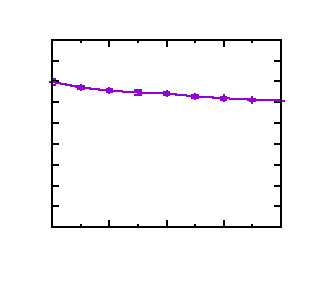
\includegraphics{Histo-lock-local-96-itu-desktop}}%
    \gplfronttext
  \end{picture}%
\endgroup

		\caption{96 bytes}
	\end{subfigure}
	\begin{subfigure}{0.32\textwidth}
		% GNUPLOT: LaTeX picture with Postscript
\begingroup
  \makeatletter
  \providecommand\color[2][]{%
    \GenericError{(gnuplot) \space\space\space\@spaces}{%
      Package color not loaded in conjunction with
      terminal option `colourtext'%
    }{See the gnuplot documentation for explanation.%
    }{Either use 'blacktext' in gnuplot or load the package
      color.sty in LaTeX.}%
    \renewcommand\color[2][]{}%
  }%
  \providecommand\includegraphics[2][]{%
    \GenericError{(gnuplot) \space\space\space\@spaces}{%
      Package graphicx or graphics not loaded%
    }{See the gnuplot documentation for explanation.%
    }{The gnuplot epslatex terminal needs graphicx.sty or graphics.sty.}%
    \renewcommand\includegraphics[2][]{}%
  }%
  \providecommand\rotatebox[2]{#2}%
  \@ifundefined{ifGPcolor}{%
    \newif\ifGPcolor
    \GPcolorfalse
  }{}%
  \@ifundefined{ifGPblacktext}{%
    \newif\ifGPblacktext
    \GPblacktexttrue
  }{}%
  % define a \g@addto@macro without @ in the name:
  \let\gplgaddtomacro\g@addto@macro
  % define empty templates for all commands taking text:
  \gdef\gplbacktext{}%
  \gdef\gplfronttext{}%
  \makeatother
  \ifGPblacktext
    % no textcolor at all
    \def\colorrgb#1{}%
    \def\colorgray#1{}%
  \else
    % gray or color?
    \ifGPcolor
      \def\colorrgb#1{\color[rgb]{#1}}%
      \def\colorgray#1{\color[gray]{#1}}%
      \expandafter\def\csname LTw\endcsname{\color{white}}%
      \expandafter\def\csname LTb\endcsname{\color{black}}%
      \expandafter\def\csname LTa\endcsname{\color{black}}%
      \expandafter\def\csname LT0\endcsname{\color[rgb]{1,0,0}}%
      \expandafter\def\csname LT1\endcsname{\color[rgb]{0,1,0}}%
      \expandafter\def\csname LT2\endcsname{\color[rgb]{0,0,1}}%
      \expandafter\def\csname LT3\endcsname{\color[rgb]{1,0,1}}%
      \expandafter\def\csname LT4\endcsname{\color[rgb]{0,1,1}}%
      \expandafter\def\csname LT5\endcsname{\color[rgb]{1,1,0}}%
      \expandafter\def\csname LT6\endcsname{\color[rgb]{0,0,0}}%
      \expandafter\def\csname LT7\endcsname{\color[rgb]{1,0.3,0}}%
      \expandafter\def\csname LT8\endcsname{\color[rgb]{0.5,0.5,0.5}}%
    \else
      % gray
      \def\colorrgb#1{\color{black}}%
      \def\colorgray#1{\color[gray]{#1}}%
      \expandafter\def\csname LTw\endcsname{\color{white}}%
      \expandafter\def\csname LTb\endcsname{\color{black}}%
      \expandafter\def\csname LTa\endcsname{\color{black}}%
      \expandafter\def\csname LT0\endcsname{\color{black}}%
      \expandafter\def\csname LT1\endcsname{\color{black}}%
      \expandafter\def\csname LT2\endcsname{\color{black}}%
      \expandafter\def\csname LT3\endcsname{\color{black}}%
      \expandafter\def\csname LT4\endcsname{\color{black}}%
      \expandafter\def\csname LT5\endcsname{\color{black}}%
      \expandafter\def\csname LT6\endcsname{\color{black}}%
      \expandafter\def\csname LT7\endcsname{\color{black}}%
      \expandafter\def\csname LT8\endcsname{\color{black}}%
    \fi
  \fi
    \setlength{\unitlength}{0.0500bp}%
    \ifx\gptboxheight\undefined%
      \newlength{\gptboxheight}%
      \newlength{\gptboxwidth}%
      \newsavebox{\gptboxtext}%
    \fi%
    \setlength{\fboxrule}{0.5pt}%
    \setlength{\fboxsep}{1pt}%
\begin{picture}(2880.00,2520.00)%
    \gplgaddtomacro\gplbacktext{%
      \csname LTb\endcsname%%
      \put(211,700){\makebox(0,0)[r]{\strut{}}}%
      \put(211,900){\makebox(0,0)[r]{\strut{}}}%
      \put(211,1100){\makebox(0,0)[r]{\strut{}}}%
      \put(211,1300){\makebox(0,0)[r]{\strut{}}}%
      \put(211,1500){\makebox(0,0)[r]{\strut{}}}%
      \put(211,1700){\makebox(0,0)[r]{\strut{}}}%
      \put(211,1900){\makebox(0,0)[r]{\strut{}}}%
      \put(211,2100){\makebox(0,0)[r]{\strut{}}}%
      \put(211,2300){\makebox(0,0)[r]{\strut{}}}%
      \put(343,368){\rotatebox{45}{\makebox(0,0)[r]{\strut{}$0$}}}%
      \put(891,368){\rotatebox{45}{\makebox(0,0)[r]{\strut{}$32$}}}%
      \put(1440,368){\rotatebox{45}{\makebox(0,0)[r]{\strut{}$64$}}}%
      \put(1988,368){\rotatebox{45}{\makebox(0,0)[r]{\strut{}$96$}}}%
      \put(2536,368){\rotatebox{45}{\makebox(0,0)[r]{\strut{}$128$}}}%
    }%
    \gplgaddtomacro\gplfronttext{%
    }%
    \gplbacktext
    \put(0,0){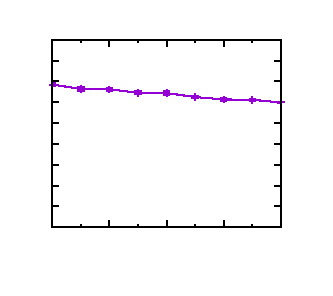
\includegraphics{Histo-lock-local-112-itu-desktop}}%
    \gplfronttext
  \end{picture}%
\endgroup

		\caption{112 bytes}
	\end{subfigure}
	\begin{subfigure}{0.32\textwidth}
		% GNUPLOT: LaTeX picture with Postscript
\begingroup
  \makeatletter
  \providecommand\color[2][]{%
    \GenericError{(gnuplot) \space\space\space\@spaces}{%
      Package color not loaded in conjunction with
      terminal option `colourtext'%
    }{See the gnuplot documentation for explanation.%
    }{Either use 'blacktext' in gnuplot or load the package
      color.sty in LaTeX.}%
    \renewcommand\color[2][]{}%
  }%
  \providecommand\includegraphics[2][]{%
    \GenericError{(gnuplot) \space\space\space\@spaces}{%
      Package graphicx or graphics not loaded%
    }{See the gnuplot documentation for explanation.%
    }{The gnuplot epslatex terminal needs graphicx.sty or graphics.sty.}%
    \renewcommand\includegraphics[2][]{}%
  }%
  \providecommand\rotatebox[2]{#2}%
  \@ifundefined{ifGPcolor}{%
    \newif\ifGPcolor
    \GPcolorfalse
  }{}%
  \@ifundefined{ifGPblacktext}{%
    \newif\ifGPblacktext
    \GPblacktexttrue
  }{}%
  % define a \g@addto@macro without @ in the name:
  \let\gplgaddtomacro\g@addto@macro
  % define empty templates for all commands taking text:
  \gdef\gplbacktext{}%
  \gdef\gplfronttext{}%
  \makeatother
  \ifGPblacktext
    % no textcolor at all
    \def\colorrgb#1{}%
    \def\colorgray#1{}%
  \else
    % gray or color?
    \ifGPcolor
      \def\colorrgb#1{\color[rgb]{#1}}%
      \def\colorgray#1{\color[gray]{#1}}%
      \expandafter\def\csname LTw\endcsname{\color{white}}%
      \expandafter\def\csname LTb\endcsname{\color{black}}%
      \expandafter\def\csname LTa\endcsname{\color{black}}%
      \expandafter\def\csname LT0\endcsname{\color[rgb]{1,0,0}}%
      \expandafter\def\csname LT1\endcsname{\color[rgb]{0,1,0}}%
      \expandafter\def\csname LT2\endcsname{\color[rgb]{0,0,1}}%
      \expandafter\def\csname LT3\endcsname{\color[rgb]{1,0,1}}%
      \expandafter\def\csname LT4\endcsname{\color[rgb]{0,1,1}}%
      \expandafter\def\csname LT5\endcsname{\color[rgb]{1,1,0}}%
      \expandafter\def\csname LT6\endcsname{\color[rgb]{0,0,0}}%
      \expandafter\def\csname LT7\endcsname{\color[rgb]{1,0.3,0}}%
      \expandafter\def\csname LT8\endcsname{\color[rgb]{0.5,0.5,0.5}}%
    \else
      % gray
      \def\colorrgb#1{\color{black}}%
      \def\colorgray#1{\color[gray]{#1}}%
      \expandafter\def\csname LTw\endcsname{\color{white}}%
      \expandafter\def\csname LTb\endcsname{\color{black}}%
      \expandafter\def\csname LTa\endcsname{\color{black}}%
      \expandafter\def\csname LT0\endcsname{\color{black}}%
      \expandafter\def\csname LT1\endcsname{\color{black}}%
      \expandafter\def\csname LT2\endcsname{\color{black}}%
      \expandafter\def\csname LT3\endcsname{\color{black}}%
      \expandafter\def\csname LT4\endcsname{\color{black}}%
      \expandafter\def\csname LT5\endcsname{\color{black}}%
      \expandafter\def\csname LT6\endcsname{\color{black}}%
      \expandafter\def\csname LT7\endcsname{\color{black}}%
      \expandafter\def\csname LT8\endcsname{\color{black}}%
    \fi
  \fi
    \setlength{\unitlength}{0.0500bp}%
    \ifx\gptboxheight\undefined%
      \newlength{\gptboxheight}%
      \newlength{\gptboxwidth}%
      \newsavebox{\gptboxtext}%
    \fi%
    \setlength{\fboxrule}{0.5pt}%
    \setlength{\fboxsep}{1pt}%
\begin{picture}(2880.00,2520.00)%
    \gplgaddtomacro\gplbacktext{%
      \csname LTb\endcsname%%
      \put(198,700){\makebox(0,0)[r]{\strut{}}}%
      \put(198,900){\makebox(0,0)[r]{\strut{}}}%
      \put(198,1100){\makebox(0,0)[r]{\strut{}}}%
      \put(198,1300){\makebox(0,0)[r]{\strut{}}}%
      \put(198,1500){\makebox(0,0)[r]{\strut{}}}%
      \put(198,1700){\makebox(0,0)[r]{\strut{}}}%
      \put(198,1900){\makebox(0,0)[r]{\strut{}}}%
      \put(198,2100){\makebox(0,0)[r]{\strut{}}}%
      \put(198,2300){\makebox(0,0)[r]{\strut{}}}%
      \put(330,368){\rotatebox{45}{\makebox(0,0)[r]{\strut{}$0$}}}%
      \put(868,368){\rotatebox{45}{\makebox(0,0)[r]{\strut{}$32$}}}%
      \put(1407,368){\rotatebox{45}{\makebox(0,0)[r]{\strut{}$64$}}}%
      \put(1945,368){\rotatebox{45}{\makebox(0,0)[r]{\strut{}$96$}}}%
      \put(2483,368){\rotatebox{45}{\makebox(0,0)[r]{\strut{}$128$}}}%
    }%
    \gplgaddtomacro\gplfronttext{%
    }%
    \gplbacktext
    \put(0,0){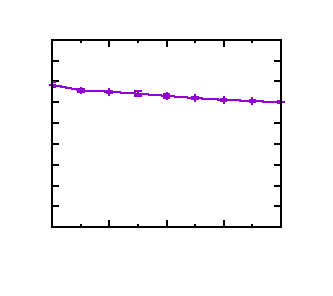
\includegraphics{Histo-lock-local-128-itu-desktop}}%
    \gplfronttext
  \end{picture}%
\endgroup

		\caption{128 bytes}
	\end{subfigure}
	\caption{The histogram problem on the i7 platform. Each plot uses a
	different amount of padding between the locks (specified beneath each
	plot). The plots show the running time of the histogram problem (each
	tick is 10 milliseconds. The axis starts at 0) as a function of the amount of padding between
	the histogram buckets in bytes.}
\end{figure}

\begin{figure}[hbpt]
	\graphicspath{{plots/}}
	\begin{subfigure}{0.32\textwidth}
		% GNUPLOT: LaTeX picture with Postscript
\begingroup
  \makeatletter
  \providecommand\color[2][]{%
    \GenericError{(gnuplot) \space\space\space\@spaces}{%
      Package color not loaded in conjunction with
      terminal option `colourtext'%
    }{See the gnuplot documentation for explanation.%
    }{Either use 'blacktext' in gnuplot or load the package
      color.sty in LaTeX.}%
    \renewcommand\color[2][]{}%
  }%
  \providecommand\includegraphics[2][]{%
    \GenericError{(gnuplot) \space\space\space\@spaces}{%
      Package graphicx or graphics not loaded%
    }{See the gnuplot documentation for explanation.%
    }{The gnuplot epslatex terminal needs graphicx.sty or graphics.sty.}%
    \renewcommand\includegraphics[2][]{}%
  }%
  \providecommand\rotatebox[2]{#2}%
  \@ifundefined{ifGPcolor}{%
    \newif\ifGPcolor
    \GPcolorfalse
  }{}%
  \@ifundefined{ifGPblacktext}{%
    \newif\ifGPblacktext
    \GPblacktexttrue
  }{}%
  % define a \g@addto@macro without @ in the name:
  \let\gplgaddtomacro\g@addto@macro
  % define empty templates for all commands taking text:
  \gdef\gplbacktext{}%
  \gdef\gplfronttext{}%
  \makeatother
  \ifGPblacktext
    % no textcolor at all
    \def\colorrgb#1{}%
    \def\colorgray#1{}%
  \else
    % gray or color?
    \ifGPcolor
      \def\colorrgb#1{\color[rgb]{#1}}%
      \def\colorgray#1{\color[gray]{#1}}%
      \expandafter\def\csname LTw\endcsname{\color{white}}%
      \expandafter\def\csname LTb\endcsname{\color{black}}%
      \expandafter\def\csname LTa\endcsname{\color{black}}%
      \expandafter\def\csname LT0\endcsname{\color[rgb]{1,0,0}}%
      \expandafter\def\csname LT1\endcsname{\color[rgb]{0,1,0}}%
      \expandafter\def\csname LT2\endcsname{\color[rgb]{0,0,1}}%
      \expandafter\def\csname LT3\endcsname{\color[rgb]{1,0,1}}%
      \expandafter\def\csname LT4\endcsname{\color[rgb]{0,1,1}}%
      \expandafter\def\csname LT5\endcsname{\color[rgb]{1,1,0}}%
      \expandafter\def\csname LT6\endcsname{\color[rgb]{0,0,0}}%
      \expandafter\def\csname LT7\endcsname{\color[rgb]{1,0.3,0}}%
      \expandafter\def\csname LT8\endcsname{\color[rgb]{0.5,0.5,0.5}}%
    \else
      % gray
      \def\colorrgb#1{\color{black}}%
      \def\colorgray#1{\color[gray]{#1}}%
      \expandafter\def\csname LTw\endcsname{\color{white}}%
      \expandafter\def\csname LTb\endcsname{\color{black}}%
      \expandafter\def\csname LTa\endcsname{\color{black}}%
      \expandafter\def\csname LT0\endcsname{\color{black}}%
      \expandafter\def\csname LT1\endcsname{\color{black}}%
      \expandafter\def\csname LT2\endcsname{\color{black}}%
      \expandafter\def\csname LT3\endcsname{\color{black}}%
      \expandafter\def\csname LT4\endcsname{\color{black}}%
      \expandafter\def\csname LT5\endcsname{\color{black}}%
      \expandafter\def\csname LT6\endcsname{\color{black}}%
      \expandafter\def\csname LT7\endcsname{\color{black}}%
      \expandafter\def\csname LT8\endcsname{\color{black}}%
    \fi
  \fi
    \setlength{\unitlength}{0.0500bp}%
    \ifx\gptboxheight\undefined%
      \newlength{\gptboxheight}%
      \newlength{\gptboxwidth}%
      \newsavebox{\gptboxtext}%
    \fi%
    \setlength{\fboxrule}{0.5pt}%
    \setlength{\fboxsep}{1pt}%
\begin{picture}(2880.00,2520.00)%
    \gplgaddtomacro\gplbacktext{%
      \csname LTb\endcsname%%
      \put(198,860){\makebox(0,0)[r]{\strut{}}}%
      \put(198,1220){\makebox(0,0)[r]{\strut{}}}%
      \put(198,1580){\makebox(0,0)[r]{\strut{}}}%
      \put(198,1940){\makebox(0,0)[r]{\strut{}}}%
      \put(198,2300){\makebox(0,0)[r]{\strut{}}}%
      \put(330,368){\rotatebox{45}{\makebox(0,0)[r]{\strut{}$0$}}}%
      \put(868,368){\rotatebox{45}{\makebox(0,0)[r]{\strut{}$32$}}}%
      \put(1407,368){\rotatebox{45}{\makebox(0,0)[r]{\strut{}$64$}}}%
      \put(1945,368){\rotatebox{45}{\makebox(0,0)[r]{\strut{}$96$}}}%
      \put(2483,368){\rotatebox{45}{\makebox(0,0)[r]{\strut{}$128$}}}%
    }%
    \gplgaddtomacro\gplfronttext{%
    }%
    \gplbacktext
    \put(0,0){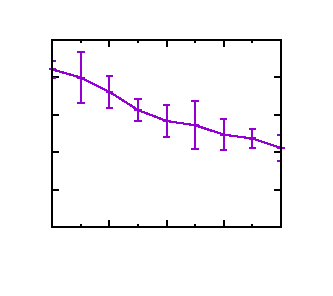
\includegraphics{Histo-lock-local-0-itu-server}}%
    \gplfronttext
  \end{picture}%
\endgroup

		\caption{0 bytes}
	\end{subfigure}
	\begin{subfigure}{0.32\textwidth}
		% GNUPLOT: LaTeX picture with Postscript
\begingroup
  \makeatletter
  \providecommand\color[2][]{%
    \GenericError{(gnuplot) \space\space\space\@spaces}{%
      Package color not loaded in conjunction with
      terminal option `colourtext'%
    }{See the gnuplot documentation for explanation.%
    }{Either use 'blacktext' in gnuplot or load the package
      color.sty in LaTeX.}%
    \renewcommand\color[2][]{}%
  }%
  \providecommand\includegraphics[2][]{%
    \GenericError{(gnuplot) \space\space\space\@spaces}{%
      Package graphicx or graphics not loaded%
    }{See the gnuplot documentation for explanation.%
    }{The gnuplot epslatex terminal needs graphicx.sty or graphics.sty.}%
    \renewcommand\includegraphics[2][]{}%
  }%
  \providecommand\rotatebox[2]{#2}%
  \@ifundefined{ifGPcolor}{%
    \newif\ifGPcolor
    \GPcolorfalse
  }{}%
  \@ifundefined{ifGPblacktext}{%
    \newif\ifGPblacktext
    \GPblacktexttrue
  }{}%
  % define a \g@addto@macro without @ in the name:
  \let\gplgaddtomacro\g@addto@macro
  % define empty templates for all commands taking text:
  \gdef\gplbacktext{}%
  \gdef\gplfronttext{}%
  \makeatother
  \ifGPblacktext
    % no textcolor at all
    \def\colorrgb#1{}%
    \def\colorgray#1{}%
  \else
    % gray or color?
    \ifGPcolor
      \def\colorrgb#1{\color[rgb]{#1}}%
      \def\colorgray#1{\color[gray]{#1}}%
      \expandafter\def\csname LTw\endcsname{\color{white}}%
      \expandafter\def\csname LTb\endcsname{\color{black}}%
      \expandafter\def\csname LTa\endcsname{\color{black}}%
      \expandafter\def\csname LT0\endcsname{\color[rgb]{1,0,0}}%
      \expandafter\def\csname LT1\endcsname{\color[rgb]{0,1,0}}%
      \expandafter\def\csname LT2\endcsname{\color[rgb]{0,0,1}}%
      \expandafter\def\csname LT3\endcsname{\color[rgb]{1,0,1}}%
      \expandafter\def\csname LT4\endcsname{\color[rgb]{0,1,1}}%
      \expandafter\def\csname LT5\endcsname{\color[rgb]{1,1,0}}%
      \expandafter\def\csname LT6\endcsname{\color[rgb]{0,0,0}}%
      \expandafter\def\csname LT7\endcsname{\color[rgb]{1,0.3,0}}%
      \expandafter\def\csname LT8\endcsname{\color[rgb]{0.5,0.5,0.5}}%
    \else
      % gray
      \def\colorrgb#1{\color{black}}%
      \def\colorgray#1{\color[gray]{#1}}%
      \expandafter\def\csname LTw\endcsname{\color{white}}%
      \expandafter\def\csname LTb\endcsname{\color{black}}%
      \expandafter\def\csname LTa\endcsname{\color{black}}%
      \expandafter\def\csname LT0\endcsname{\color{black}}%
      \expandafter\def\csname LT1\endcsname{\color{black}}%
      \expandafter\def\csname LT2\endcsname{\color{black}}%
      \expandafter\def\csname LT3\endcsname{\color{black}}%
      \expandafter\def\csname LT4\endcsname{\color{black}}%
      \expandafter\def\csname LT5\endcsname{\color{black}}%
      \expandafter\def\csname LT6\endcsname{\color{black}}%
      \expandafter\def\csname LT7\endcsname{\color{black}}%
      \expandafter\def\csname LT8\endcsname{\color{black}}%
    \fi
  \fi
    \setlength{\unitlength}{0.0500bp}%
    \ifx\gptboxheight\undefined%
      \newlength{\gptboxheight}%
      \newlength{\gptboxwidth}%
      \newsavebox{\gptboxtext}%
    \fi%
    \setlength{\fboxrule}{0.5pt}%
    \setlength{\fboxsep}{1pt}%
\begin{picture}(2376.00,2520.00)%
    \gplgaddtomacro\gplbacktext{%
      \csname LTb\endcsname%%
      \put(-40,860){\makebox(0,0)[r]{\strut{}}}%
      \put(-40,1220){\makebox(0,0)[r]{\strut{}}}%
      \put(-40,1580){\makebox(0,0)[r]{\strut{}}}%
      \put(-40,1940){\makebox(0,0)[r]{\strut{}}}%
      \put(-40,2300){\makebox(0,0)[r]{\strut{}}}%
      \put(92,368){\rotatebox{45}{\makebox(0,0)[r]{\strut{}$0$}}}%
      \put(640,368){\rotatebox{45}{\makebox(0,0)[r]{\strut{}$32$}}}%
      \put(1188,368){\rotatebox{45}{\makebox(0,0)[r]{\strut{}$64$}}}%
      \put(1735,368){\rotatebox{45}{\makebox(0,0)[r]{\strut{}$96$}}}%
      \put(2283,368){\rotatebox{45}{\makebox(0,0)[r]{\strut{}$128$}}}%
    }%
    \gplgaddtomacro\gplfronttext{%
    }%
    \gplbacktext
    \put(0,0){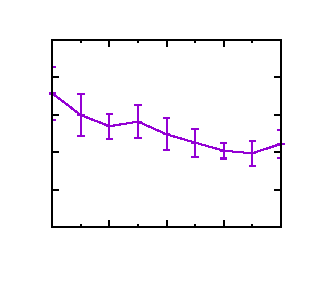
\includegraphics{Histo-lock-local-16-itu-server}}%
    \gplfronttext
  \end{picture}%
\endgroup

		\caption{16 bytes}
	\end{subfigure}
	\begin{subfigure}{0.32\textwidth}
		% GNUPLOT: LaTeX picture with Postscript
\begingroup
  \makeatletter
  \providecommand\color[2][]{%
    \GenericError{(gnuplot) \space\space\space\@spaces}{%
      Package color not loaded in conjunction with
      terminal option `colourtext'%
    }{See the gnuplot documentation for explanation.%
    }{Either use 'blacktext' in gnuplot or load the package
      color.sty in LaTeX.}%
    \renewcommand\color[2][]{}%
  }%
  \providecommand\includegraphics[2][]{%
    \GenericError{(gnuplot) \space\space\space\@spaces}{%
      Package graphicx or graphics not loaded%
    }{See the gnuplot documentation for explanation.%
    }{The gnuplot epslatex terminal needs graphicx.sty or graphics.sty.}%
    \renewcommand\includegraphics[2][]{}%
  }%
  \providecommand\rotatebox[2]{#2}%
  \@ifundefined{ifGPcolor}{%
    \newif\ifGPcolor
    \GPcolorfalse
  }{}%
  \@ifundefined{ifGPblacktext}{%
    \newif\ifGPblacktext
    \GPblacktexttrue
  }{}%
  % define a \g@addto@macro without @ in the name:
  \let\gplgaddtomacro\g@addto@macro
  % define empty templates for all commands taking text:
  \gdef\gplbacktext{}%
  \gdef\gplfronttext{}%
  \makeatother
  \ifGPblacktext
    % no textcolor at all
    \def\colorrgb#1{}%
    \def\colorgray#1{}%
  \else
    % gray or color?
    \ifGPcolor
      \def\colorrgb#1{\color[rgb]{#1}}%
      \def\colorgray#1{\color[gray]{#1}}%
      \expandafter\def\csname LTw\endcsname{\color{white}}%
      \expandafter\def\csname LTb\endcsname{\color{black}}%
      \expandafter\def\csname LTa\endcsname{\color{black}}%
      \expandafter\def\csname LT0\endcsname{\color[rgb]{1,0,0}}%
      \expandafter\def\csname LT1\endcsname{\color[rgb]{0,1,0}}%
      \expandafter\def\csname LT2\endcsname{\color[rgb]{0,0,1}}%
      \expandafter\def\csname LT3\endcsname{\color[rgb]{1,0,1}}%
      \expandafter\def\csname LT4\endcsname{\color[rgb]{0,1,1}}%
      \expandafter\def\csname LT5\endcsname{\color[rgb]{1,1,0}}%
      \expandafter\def\csname LT6\endcsname{\color[rgb]{0,0,0}}%
      \expandafter\def\csname LT7\endcsname{\color[rgb]{1,0.3,0}}%
      \expandafter\def\csname LT8\endcsname{\color[rgb]{0.5,0.5,0.5}}%
    \else
      % gray
      \def\colorrgb#1{\color{black}}%
      \def\colorgray#1{\color[gray]{#1}}%
      \expandafter\def\csname LTw\endcsname{\color{white}}%
      \expandafter\def\csname LTb\endcsname{\color{black}}%
      \expandafter\def\csname LTa\endcsname{\color{black}}%
      \expandafter\def\csname LT0\endcsname{\color{black}}%
      \expandafter\def\csname LT1\endcsname{\color{black}}%
      \expandafter\def\csname LT2\endcsname{\color{black}}%
      \expandafter\def\csname LT3\endcsname{\color{black}}%
      \expandafter\def\csname LT4\endcsname{\color{black}}%
      \expandafter\def\csname LT5\endcsname{\color{black}}%
      \expandafter\def\csname LT6\endcsname{\color{black}}%
      \expandafter\def\csname LT7\endcsname{\color{black}}%
      \expandafter\def\csname LT8\endcsname{\color{black}}%
    \fi
  \fi
    \setlength{\unitlength}{0.0500bp}%
    \ifx\gptboxheight\undefined%
      \newlength{\gptboxheight}%
      \newlength{\gptboxwidth}%
      \newsavebox{\gptboxtext}%
    \fi%
    \setlength{\fboxrule}{0.5pt}%
    \setlength{\fboxsep}{1pt}%
\begin{picture}(2880.00,2520.00)%
    \gplgaddtomacro\gplbacktext{%
      \csname LTb\endcsname%%
      \put(198,860){\makebox(0,0)[r]{\strut{}}}%
      \put(198,1220){\makebox(0,0)[r]{\strut{}}}%
      \put(198,1580){\makebox(0,0)[r]{\strut{}}}%
      \put(198,1940){\makebox(0,0)[r]{\strut{}}}%
      \put(198,2300){\makebox(0,0)[r]{\strut{}}}%
      \put(330,368){\rotatebox{45}{\makebox(0,0)[r]{\strut{}$0$}}}%
      \put(868,368){\rotatebox{45}{\makebox(0,0)[r]{\strut{}$32$}}}%
      \put(1407,368){\rotatebox{45}{\makebox(0,0)[r]{\strut{}$64$}}}%
      \put(1945,368){\rotatebox{45}{\makebox(0,0)[r]{\strut{}$96$}}}%
      \put(2483,368){\rotatebox{45}{\makebox(0,0)[r]{\strut{}$128$}}}%
    }%
    \gplgaddtomacro\gplfronttext{%
    }%
    \gplbacktext
    \put(0,0){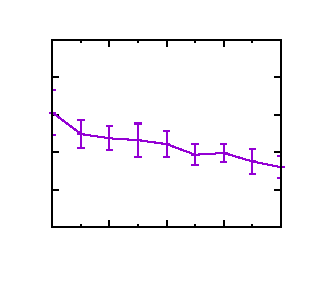
\includegraphics{Histo-lock-local-32-itu-server}}%
    \gplfronttext
  \end{picture}%
\endgroup

		\caption{32 bytes}
	\end{subfigure}
	\begin{subfigure}{0.32\textwidth}
		% GNUPLOT: LaTeX picture with Postscript
\begingroup
  \makeatletter
  \providecommand\color[2][]{%
    \GenericError{(gnuplot) \space\space\space\@spaces}{%
      Package color not loaded in conjunction with
      terminal option `colourtext'%
    }{See the gnuplot documentation for explanation.%
    }{Either use 'blacktext' in gnuplot or load the package
      color.sty in LaTeX.}%
    \renewcommand\color[2][]{}%
  }%
  \providecommand\includegraphics[2][]{%
    \GenericError{(gnuplot) \space\space\space\@spaces}{%
      Package graphicx or graphics not loaded%
    }{See the gnuplot documentation for explanation.%
    }{The gnuplot epslatex terminal needs graphicx.sty or graphics.sty.}%
    \renewcommand\includegraphics[2][]{}%
  }%
  \providecommand\rotatebox[2]{#2}%
  \@ifundefined{ifGPcolor}{%
    \newif\ifGPcolor
    \GPcolorfalse
  }{}%
  \@ifundefined{ifGPblacktext}{%
    \newif\ifGPblacktext
    \GPblacktexttrue
  }{}%
  % define a \g@addto@macro without @ in the name:
  \let\gplgaddtomacro\g@addto@macro
  % define empty templates for all commands taking text:
  \gdef\gplbacktext{}%
  \gdef\gplfronttext{}%
  \makeatother
  \ifGPblacktext
    % no textcolor at all
    \def\colorrgb#1{}%
    \def\colorgray#1{}%
  \else
    % gray or color?
    \ifGPcolor
      \def\colorrgb#1{\color[rgb]{#1}}%
      \def\colorgray#1{\color[gray]{#1}}%
      \expandafter\def\csname LTw\endcsname{\color{white}}%
      \expandafter\def\csname LTb\endcsname{\color{black}}%
      \expandafter\def\csname LTa\endcsname{\color{black}}%
      \expandafter\def\csname LT0\endcsname{\color[rgb]{1,0,0}}%
      \expandafter\def\csname LT1\endcsname{\color[rgb]{0,1,0}}%
      \expandafter\def\csname LT2\endcsname{\color[rgb]{0,0,1}}%
      \expandafter\def\csname LT3\endcsname{\color[rgb]{1,0,1}}%
      \expandafter\def\csname LT4\endcsname{\color[rgb]{0,1,1}}%
      \expandafter\def\csname LT5\endcsname{\color[rgb]{1,1,0}}%
      \expandafter\def\csname LT6\endcsname{\color[rgb]{0,0,0}}%
      \expandafter\def\csname LT7\endcsname{\color[rgb]{1,0.3,0}}%
      \expandafter\def\csname LT8\endcsname{\color[rgb]{0.5,0.5,0.5}}%
    \else
      % gray
      \def\colorrgb#1{\color{black}}%
      \def\colorgray#1{\color[gray]{#1}}%
      \expandafter\def\csname LTw\endcsname{\color{white}}%
      \expandafter\def\csname LTb\endcsname{\color{black}}%
      \expandafter\def\csname LTa\endcsname{\color{black}}%
      \expandafter\def\csname LT0\endcsname{\color{black}}%
      \expandafter\def\csname LT1\endcsname{\color{black}}%
      \expandafter\def\csname LT2\endcsname{\color{black}}%
      \expandafter\def\csname LT3\endcsname{\color{black}}%
      \expandafter\def\csname LT4\endcsname{\color{black}}%
      \expandafter\def\csname LT5\endcsname{\color{black}}%
      \expandafter\def\csname LT6\endcsname{\color{black}}%
      \expandafter\def\csname LT7\endcsname{\color{black}}%
      \expandafter\def\csname LT8\endcsname{\color{black}}%
    \fi
  \fi
    \setlength{\unitlength}{0.0500bp}%
    \ifx\gptboxheight\undefined%
      \newlength{\gptboxheight}%
      \newlength{\gptboxwidth}%
      \newsavebox{\gptboxtext}%
    \fi%
    \setlength{\fboxrule}{0.5pt}%
    \setlength{\fboxsep}{1pt}%
\begin{picture}(2376.00,2520.00)%
    \gplgaddtomacro\gplbacktext{%
      \csname LTb\endcsname%%
      \put(-40,860){\makebox(0,0)[r]{\strut{}}}%
      \put(-40,1220){\makebox(0,0)[r]{\strut{}}}%
      \put(-40,1580){\makebox(0,0)[r]{\strut{}}}%
      \put(-40,1940){\makebox(0,0)[r]{\strut{}}}%
      \put(-40,2300){\makebox(0,0)[r]{\strut{}}}%
      \put(92,368){\rotatebox{45}{\makebox(0,0)[r]{\strut{}$0$}}}%
      \put(640,368){\rotatebox{45}{\makebox(0,0)[r]{\strut{}$32$}}}%
      \put(1188,368){\rotatebox{45}{\makebox(0,0)[r]{\strut{}$64$}}}%
      \put(1735,368){\rotatebox{45}{\makebox(0,0)[r]{\strut{}$96$}}}%
      \put(2283,368){\rotatebox{45}{\makebox(0,0)[r]{\strut{}$128$}}}%
    }%
    \gplgaddtomacro\gplfronttext{%
    }%
    \gplbacktext
    \put(0,0){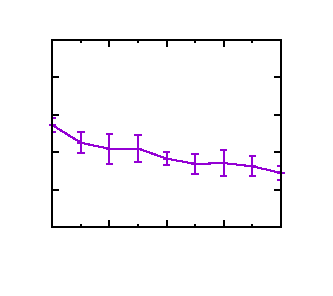
\includegraphics{Histo-lock-local-48-itu-server}}%
    \gplfronttext
  \end{picture}%
\endgroup

		\caption{48 bytes}
	\end{subfigure}
	\begin{subfigure}{0.32\textwidth}
		% GNUPLOT: LaTeX picture with Postscript
\begingroup
  \makeatletter
  \providecommand\color[2][]{%
    \GenericError{(gnuplot) \space\space\space\@spaces}{%
      Package color not loaded in conjunction with
      terminal option `colourtext'%
    }{See the gnuplot documentation for explanation.%
    }{Either use 'blacktext' in gnuplot or load the package
      color.sty in LaTeX.}%
    \renewcommand\color[2][]{}%
  }%
  \providecommand\includegraphics[2][]{%
    \GenericError{(gnuplot) \space\space\space\@spaces}{%
      Package graphicx or graphics not loaded%
    }{See the gnuplot documentation for explanation.%
    }{The gnuplot epslatex terminal needs graphicx.sty or graphics.sty.}%
    \renewcommand\includegraphics[2][]{}%
  }%
  \providecommand\rotatebox[2]{#2}%
  \@ifundefined{ifGPcolor}{%
    \newif\ifGPcolor
    \GPcolorfalse
  }{}%
  \@ifundefined{ifGPblacktext}{%
    \newif\ifGPblacktext
    \GPblacktexttrue
  }{}%
  % define a \g@addto@macro without @ in the name:
  \let\gplgaddtomacro\g@addto@macro
  % define empty templates for all commands taking text:
  \gdef\gplbacktext{}%
  \gdef\gplfronttext{}%
  \makeatother
  \ifGPblacktext
    % no textcolor at all
    \def\colorrgb#1{}%
    \def\colorgray#1{}%
  \else
    % gray or color?
    \ifGPcolor
      \def\colorrgb#1{\color[rgb]{#1}}%
      \def\colorgray#1{\color[gray]{#1}}%
      \expandafter\def\csname LTw\endcsname{\color{white}}%
      \expandafter\def\csname LTb\endcsname{\color{black}}%
      \expandafter\def\csname LTa\endcsname{\color{black}}%
      \expandafter\def\csname LT0\endcsname{\color[rgb]{1,0,0}}%
      \expandafter\def\csname LT1\endcsname{\color[rgb]{0,1,0}}%
      \expandafter\def\csname LT2\endcsname{\color[rgb]{0,0,1}}%
      \expandafter\def\csname LT3\endcsname{\color[rgb]{1,0,1}}%
      \expandafter\def\csname LT4\endcsname{\color[rgb]{0,1,1}}%
      \expandafter\def\csname LT5\endcsname{\color[rgb]{1,1,0}}%
      \expandafter\def\csname LT6\endcsname{\color[rgb]{0,0,0}}%
      \expandafter\def\csname LT7\endcsname{\color[rgb]{1,0.3,0}}%
      \expandafter\def\csname LT8\endcsname{\color[rgb]{0.5,0.5,0.5}}%
    \else
      % gray
      \def\colorrgb#1{\color{black}}%
      \def\colorgray#1{\color[gray]{#1}}%
      \expandafter\def\csname LTw\endcsname{\color{white}}%
      \expandafter\def\csname LTb\endcsname{\color{black}}%
      \expandafter\def\csname LTa\endcsname{\color{black}}%
      \expandafter\def\csname LT0\endcsname{\color{black}}%
      \expandafter\def\csname LT1\endcsname{\color{black}}%
      \expandafter\def\csname LT2\endcsname{\color{black}}%
      \expandafter\def\csname LT3\endcsname{\color{black}}%
      \expandafter\def\csname LT4\endcsname{\color{black}}%
      \expandafter\def\csname LT5\endcsname{\color{black}}%
      \expandafter\def\csname LT6\endcsname{\color{black}}%
      \expandafter\def\csname LT7\endcsname{\color{black}}%
      \expandafter\def\csname LT8\endcsname{\color{black}}%
    \fi
  \fi
    \setlength{\unitlength}{0.0500bp}%
    \ifx\gptboxheight\undefined%
      \newlength{\gptboxheight}%
      \newlength{\gptboxwidth}%
      \newsavebox{\gptboxtext}%
    \fi%
    \setlength{\fboxrule}{0.5pt}%
    \setlength{\fboxsep}{1pt}%
\begin{picture}(2880.00,2520.00)%
    \gplgaddtomacro\gplbacktext{%
      \csname LTb\endcsname%%
      \put(211,860){\makebox(0,0)[r]{\strut{}}}%
      \put(211,1220){\makebox(0,0)[r]{\strut{}}}%
      \put(211,1580){\makebox(0,0)[r]{\strut{}}}%
      \put(211,1940){\makebox(0,0)[r]{\strut{}}}%
      \put(211,2300){\makebox(0,0)[r]{\strut{}}}%
      \put(343,368){\rotatebox{45}{\makebox(0,0)[r]{\strut{}$0$}}}%
      \put(891,368){\rotatebox{45}{\makebox(0,0)[r]{\strut{}$32$}}}%
      \put(1440,368){\rotatebox{45}{\makebox(0,0)[r]{\strut{}$64$}}}%
      \put(1988,368){\rotatebox{45}{\makebox(0,0)[r]{\strut{}$96$}}}%
      \put(2536,368){\rotatebox{45}{\makebox(0,0)[r]{\strut{}$128$}}}%
    }%
    \gplgaddtomacro\gplfronttext{%
    }%
    \gplbacktext
    \put(0,0){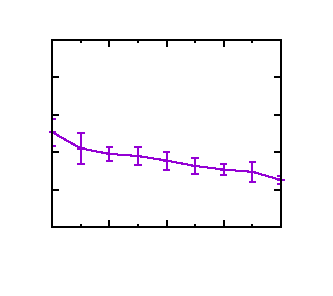
\includegraphics{Histo-lock-local-64-itu-server}}%
    \gplfronttext
  \end{picture}%
\endgroup

		\caption{64 bytes}
	\end{subfigure}
	\begin{subfigure}{0.32\textwidth}
		% GNUPLOT: LaTeX picture with Postscript
\begingroup
  \makeatletter
  \providecommand\color[2][]{%
    \GenericError{(gnuplot) \space\space\space\@spaces}{%
      Package color not loaded in conjunction with
      terminal option `colourtext'%
    }{See the gnuplot documentation for explanation.%
    }{Either use 'blacktext' in gnuplot or load the package
      color.sty in LaTeX.}%
    \renewcommand\color[2][]{}%
  }%
  \providecommand\includegraphics[2][]{%
    \GenericError{(gnuplot) \space\space\space\@spaces}{%
      Package graphicx or graphics not loaded%
    }{See the gnuplot documentation for explanation.%
    }{The gnuplot epslatex terminal needs graphicx.sty or graphics.sty.}%
    \renewcommand\includegraphics[2][]{}%
  }%
  \providecommand\rotatebox[2]{#2}%
  \@ifundefined{ifGPcolor}{%
    \newif\ifGPcolor
    \GPcolorfalse
  }{}%
  \@ifundefined{ifGPblacktext}{%
    \newif\ifGPblacktext
    \GPblacktexttrue
  }{}%
  % define a \g@addto@macro without @ in the name:
  \let\gplgaddtomacro\g@addto@macro
  % define empty templates for all commands taking text:
  \gdef\gplbacktext{}%
  \gdef\gplfronttext{}%
  \makeatother
  \ifGPblacktext
    % no textcolor at all
    \def\colorrgb#1{}%
    \def\colorgray#1{}%
  \else
    % gray or color?
    \ifGPcolor
      \def\colorrgb#1{\color[rgb]{#1}}%
      \def\colorgray#1{\color[gray]{#1}}%
      \expandafter\def\csname LTw\endcsname{\color{white}}%
      \expandafter\def\csname LTb\endcsname{\color{black}}%
      \expandafter\def\csname LTa\endcsname{\color{black}}%
      \expandafter\def\csname LT0\endcsname{\color[rgb]{1,0,0}}%
      \expandafter\def\csname LT1\endcsname{\color[rgb]{0,1,0}}%
      \expandafter\def\csname LT2\endcsname{\color[rgb]{0,0,1}}%
      \expandafter\def\csname LT3\endcsname{\color[rgb]{1,0,1}}%
      \expandafter\def\csname LT4\endcsname{\color[rgb]{0,1,1}}%
      \expandafter\def\csname LT5\endcsname{\color[rgb]{1,1,0}}%
      \expandafter\def\csname LT6\endcsname{\color[rgb]{0,0,0}}%
      \expandafter\def\csname LT7\endcsname{\color[rgb]{1,0.3,0}}%
      \expandafter\def\csname LT8\endcsname{\color[rgb]{0.5,0.5,0.5}}%
    \else
      % gray
      \def\colorrgb#1{\color{black}}%
      \def\colorgray#1{\color[gray]{#1}}%
      \expandafter\def\csname LTw\endcsname{\color{white}}%
      \expandafter\def\csname LTb\endcsname{\color{black}}%
      \expandafter\def\csname LTa\endcsname{\color{black}}%
      \expandafter\def\csname LT0\endcsname{\color{black}}%
      \expandafter\def\csname LT1\endcsname{\color{black}}%
      \expandafter\def\csname LT2\endcsname{\color{black}}%
      \expandafter\def\csname LT3\endcsname{\color{black}}%
      \expandafter\def\csname LT4\endcsname{\color{black}}%
      \expandafter\def\csname LT5\endcsname{\color{black}}%
      \expandafter\def\csname LT6\endcsname{\color{black}}%
      \expandafter\def\csname LT7\endcsname{\color{black}}%
      \expandafter\def\csname LT8\endcsname{\color{black}}%
    \fi
  \fi
    \setlength{\unitlength}{0.0500bp}%
    \ifx\gptboxheight\undefined%
      \newlength{\gptboxheight}%
      \newlength{\gptboxwidth}%
      \newsavebox{\gptboxtext}%
    \fi%
    \setlength{\fboxrule}{0.5pt}%
    \setlength{\fboxsep}{1pt}%
\begin{picture}(2376.00,2520.00)%
    \gplgaddtomacro\gplbacktext{%
      \csname LTb\endcsname%%
      \put(-40,860){\makebox(0,0)[r]{\strut{}}}%
      \put(-40,1220){\makebox(0,0)[r]{\strut{}}}%
      \put(-40,1580){\makebox(0,0)[r]{\strut{}}}%
      \put(-40,1940){\makebox(0,0)[r]{\strut{}}}%
      \put(-40,2300){\makebox(0,0)[r]{\strut{}}}%
      \put(92,368){\rotatebox{45}{\makebox(0,0)[r]{\strut{}$0$}}}%
      \put(640,368){\rotatebox{45}{\makebox(0,0)[r]{\strut{}$32$}}}%
      \put(1188,368){\rotatebox{45}{\makebox(0,0)[r]{\strut{}$64$}}}%
      \put(1735,368){\rotatebox{45}{\makebox(0,0)[r]{\strut{}$96$}}}%
      \put(2283,368){\rotatebox{45}{\makebox(0,0)[r]{\strut{}$128$}}}%
    }%
    \gplgaddtomacro\gplfronttext{%
    }%
    \gplbacktext
    \put(0,0){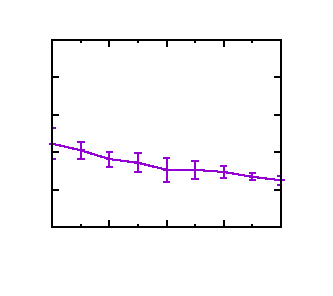
\includegraphics{Histo-lock-local-80-itu-server}}%
    \gplfronttext
  \end{picture}%
\endgroup

		\caption{80 bytes}
	\end{subfigure}
	\begin{subfigure}{0.32\textwidth}
		% GNUPLOT: LaTeX picture with Postscript
\begingroup
  \makeatletter
  \providecommand\color[2][]{%
    \GenericError{(gnuplot) \space\space\space\@spaces}{%
      Package color not loaded in conjunction with
      terminal option `colourtext'%
    }{See the gnuplot documentation for explanation.%
    }{Either use 'blacktext' in gnuplot or load the package
      color.sty in LaTeX.}%
    \renewcommand\color[2][]{}%
  }%
  \providecommand\includegraphics[2][]{%
    \GenericError{(gnuplot) \space\space\space\@spaces}{%
      Package graphicx or graphics not loaded%
    }{See the gnuplot documentation for explanation.%
    }{The gnuplot epslatex terminal needs graphicx.sty or graphics.sty.}%
    \renewcommand\includegraphics[2][]{}%
  }%
  \providecommand\rotatebox[2]{#2}%
  \@ifundefined{ifGPcolor}{%
    \newif\ifGPcolor
    \GPcolorfalse
  }{}%
  \@ifundefined{ifGPblacktext}{%
    \newif\ifGPblacktext
    \GPblacktexttrue
  }{}%
  % define a \g@addto@macro without @ in the name:
  \let\gplgaddtomacro\g@addto@macro
  % define empty templates for all commands taking text:
  \gdef\gplbacktext{}%
  \gdef\gplfronttext{}%
  \makeatother
  \ifGPblacktext
    % no textcolor at all
    \def\colorrgb#1{}%
    \def\colorgray#1{}%
  \else
    % gray or color?
    \ifGPcolor
      \def\colorrgb#1{\color[rgb]{#1}}%
      \def\colorgray#1{\color[gray]{#1}}%
      \expandafter\def\csname LTw\endcsname{\color{white}}%
      \expandafter\def\csname LTb\endcsname{\color{black}}%
      \expandafter\def\csname LTa\endcsname{\color{black}}%
      \expandafter\def\csname LT0\endcsname{\color[rgb]{1,0,0}}%
      \expandafter\def\csname LT1\endcsname{\color[rgb]{0,1,0}}%
      \expandafter\def\csname LT2\endcsname{\color[rgb]{0,0,1}}%
      \expandafter\def\csname LT3\endcsname{\color[rgb]{1,0,1}}%
      \expandafter\def\csname LT4\endcsname{\color[rgb]{0,1,1}}%
      \expandafter\def\csname LT5\endcsname{\color[rgb]{1,1,0}}%
      \expandafter\def\csname LT6\endcsname{\color[rgb]{0,0,0}}%
      \expandafter\def\csname LT7\endcsname{\color[rgb]{1,0.3,0}}%
      \expandafter\def\csname LT8\endcsname{\color[rgb]{0.5,0.5,0.5}}%
    \else
      % gray
      \def\colorrgb#1{\color{black}}%
      \def\colorgray#1{\color[gray]{#1}}%
      \expandafter\def\csname LTw\endcsname{\color{white}}%
      \expandafter\def\csname LTb\endcsname{\color{black}}%
      \expandafter\def\csname LTa\endcsname{\color{black}}%
      \expandafter\def\csname LT0\endcsname{\color{black}}%
      \expandafter\def\csname LT1\endcsname{\color{black}}%
      \expandafter\def\csname LT2\endcsname{\color{black}}%
      \expandafter\def\csname LT3\endcsname{\color{black}}%
      \expandafter\def\csname LT4\endcsname{\color{black}}%
      \expandafter\def\csname LT5\endcsname{\color{black}}%
      \expandafter\def\csname LT6\endcsname{\color{black}}%
      \expandafter\def\csname LT7\endcsname{\color{black}}%
      \expandafter\def\csname LT8\endcsname{\color{black}}%
    \fi
  \fi
    \setlength{\unitlength}{0.0500bp}%
    \ifx\gptboxheight\undefined%
      \newlength{\gptboxheight}%
      \newlength{\gptboxwidth}%
      \newsavebox{\gptboxtext}%
    \fi%
    \setlength{\fboxrule}{0.5pt}%
    \setlength{\fboxsep}{1pt}%
\begin{picture}(2880.00,2520.00)%
    \gplgaddtomacro\gplbacktext{%
      \csname LTb\endcsname%%
      \put(211,860){\makebox(0,0)[r]{\strut{}}}%
      \put(211,1220){\makebox(0,0)[r]{\strut{}}}%
      \put(211,1580){\makebox(0,0)[r]{\strut{}}}%
      \put(211,1940){\makebox(0,0)[r]{\strut{}}}%
      \put(211,2300){\makebox(0,0)[r]{\strut{}}}%
      \put(343,368){\rotatebox{45}{\makebox(0,0)[r]{\strut{}$0$}}}%
      \put(891,368){\rotatebox{45}{\makebox(0,0)[r]{\strut{}$32$}}}%
      \put(1440,368){\rotatebox{45}{\makebox(0,0)[r]{\strut{}$64$}}}%
      \put(1988,368){\rotatebox{45}{\makebox(0,0)[r]{\strut{}$96$}}}%
      \put(2536,368){\rotatebox{45}{\makebox(0,0)[r]{\strut{}$128$}}}%
    }%
    \gplgaddtomacro\gplfronttext{%
    }%
    \gplbacktext
    \put(0,0){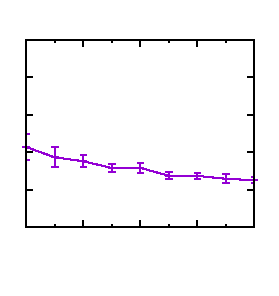
\includegraphics{Histo-lock-local-96-itu-server}}%
    \gplfronttext
  \end{picture}%
\endgroup

		\caption{96 bytes}
	\end{subfigure}
	\begin{subfigure}{0.32\textwidth}
		% GNUPLOT: LaTeX picture with Postscript
\begingroup
  \makeatletter
  \providecommand\color[2][]{%
    \GenericError{(gnuplot) \space\space\space\@spaces}{%
      Package color not loaded in conjunction with
      terminal option `colourtext'%
    }{See the gnuplot documentation for explanation.%
    }{Either use 'blacktext' in gnuplot or load the package
      color.sty in LaTeX.}%
    \renewcommand\color[2][]{}%
  }%
  \providecommand\includegraphics[2][]{%
    \GenericError{(gnuplot) \space\space\space\@spaces}{%
      Package graphicx or graphics not loaded%
    }{See the gnuplot documentation for explanation.%
    }{The gnuplot epslatex terminal needs graphicx.sty or graphics.sty.}%
    \renewcommand\includegraphics[2][]{}%
  }%
  \providecommand\rotatebox[2]{#2}%
  \@ifundefined{ifGPcolor}{%
    \newif\ifGPcolor
    \GPcolorfalse
  }{}%
  \@ifundefined{ifGPblacktext}{%
    \newif\ifGPblacktext
    \GPblacktexttrue
  }{}%
  % define a \g@addto@macro without @ in the name:
  \let\gplgaddtomacro\g@addto@macro
  % define empty templates for all commands taking text:
  \gdef\gplbacktext{}%
  \gdef\gplfronttext{}%
  \makeatother
  \ifGPblacktext
    % no textcolor at all
    \def\colorrgb#1{}%
    \def\colorgray#1{}%
  \else
    % gray or color?
    \ifGPcolor
      \def\colorrgb#1{\color[rgb]{#1}}%
      \def\colorgray#1{\color[gray]{#1}}%
      \expandafter\def\csname LTw\endcsname{\color{white}}%
      \expandafter\def\csname LTb\endcsname{\color{black}}%
      \expandafter\def\csname LTa\endcsname{\color{black}}%
      \expandafter\def\csname LT0\endcsname{\color[rgb]{1,0,0}}%
      \expandafter\def\csname LT1\endcsname{\color[rgb]{0,1,0}}%
      \expandafter\def\csname LT2\endcsname{\color[rgb]{0,0,1}}%
      \expandafter\def\csname LT3\endcsname{\color[rgb]{1,0,1}}%
      \expandafter\def\csname LT4\endcsname{\color[rgb]{0,1,1}}%
      \expandafter\def\csname LT5\endcsname{\color[rgb]{1,1,0}}%
      \expandafter\def\csname LT6\endcsname{\color[rgb]{0,0,0}}%
      \expandafter\def\csname LT7\endcsname{\color[rgb]{1,0.3,0}}%
      \expandafter\def\csname LT8\endcsname{\color[rgb]{0.5,0.5,0.5}}%
    \else
      % gray
      \def\colorrgb#1{\color{black}}%
      \def\colorgray#1{\color[gray]{#1}}%
      \expandafter\def\csname LTw\endcsname{\color{white}}%
      \expandafter\def\csname LTb\endcsname{\color{black}}%
      \expandafter\def\csname LTa\endcsname{\color{black}}%
      \expandafter\def\csname LT0\endcsname{\color{black}}%
      \expandafter\def\csname LT1\endcsname{\color{black}}%
      \expandafter\def\csname LT2\endcsname{\color{black}}%
      \expandafter\def\csname LT3\endcsname{\color{black}}%
      \expandafter\def\csname LT4\endcsname{\color{black}}%
      \expandafter\def\csname LT5\endcsname{\color{black}}%
      \expandafter\def\csname LT6\endcsname{\color{black}}%
      \expandafter\def\csname LT7\endcsname{\color{black}}%
      \expandafter\def\csname LT8\endcsname{\color{black}}%
    \fi
  \fi
    \setlength{\unitlength}{0.0500bp}%
    \ifx\gptboxheight\undefined%
      \newlength{\gptboxheight}%
      \newlength{\gptboxwidth}%
      \newsavebox{\gptboxtext}%
    \fi%
    \setlength{\fboxrule}{0.5pt}%
    \setlength{\fboxsep}{1pt}%
\begin{picture}(2376.00,2520.00)%
    \gplgaddtomacro\gplbacktext{%
      \csname LTb\endcsname%%
      \put(-40,860){\makebox(0,0)[r]{\strut{}}}%
      \put(-40,1220){\makebox(0,0)[r]{\strut{}}}%
      \put(-40,1580){\makebox(0,0)[r]{\strut{}}}%
      \put(-40,1940){\makebox(0,0)[r]{\strut{}}}%
      \put(-40,2300){\makebox(0,0)[r]{\strut{}}}%
      \put(92,368){\rotatebox{45}{\makebox(0,0)[r]{\strut{}$0$}}}%
      \put(640,368){\rotatebox{45}{\makebox(0,0)[r]{\strut{}$32$}}}%
      \put(1188,368){\rotatebox{45}{\makebox(0,0)[r]{\strut{}$64$}}}%
      \put(1735,368){\rotatebox{45}{\makebox(0,0)[r]{\strut{}$96$}}}%
      \put(2283,368){\rotatebox{45}{\makebox(0,0)[r]{\strut{}$128$}}}%
    }%
    \gplgaddtomacro\gplfronttext{%
    }%
    \gplbacktext
    \put(0,0){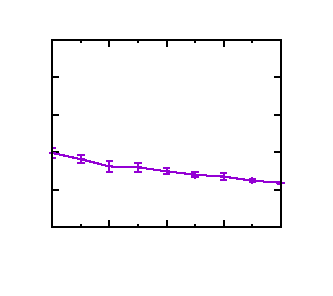
\includegraphics{Histo-lock-local-112-itu-server}}%
    \gplfronttext
  \end{picture}%
\endgroup

		\caption{112 bytes}
	\end{subfigure}
	\begin{subfigure}{0.32\textwidth}
		% GNUPLOT: LaTeX picture with Postscript
\begingroup
  \makeatletter
  \providecommand\color[2][]{%
    \GenericError{(gnuplot) \space\space\space\@spaces}{%
      Package color not loaded in conjunction with
      terminal option `colourtext'%
    }{See the gnuplot documentation for explanation.%
    }{Either use 'blacktext' in gnuplot or load the package
      color.sty in LaTeX.}%
    \renewcommand\color[2][]{}%
  }%
  \providecommand\includegraphics[2][]{%
    \GenericError{(gnuplot) \space\space\space\@spaces}{%
      Package graphicx or graphics not loaded%
    }{See the gnuplot documentation for explanation.%
    }{The gnuplot epslatex terminal needs graphicx.sty or graphics.sty.}%
    \renewcommand\includegraphics[2][]{}%
  }%
  \providecommand\rotatebox[2]{#2}%
  \@ifundefined{ifGPcolor}{%
    \newif\ifGPcolor
    \GPcolorfalse
  }{}%
  \@ifundefined{ifGPblacktext}{%
    \newif\ifGPblacktext
    \GPblacktexttrue
  }{}%
  % define a \g@addto@macro without @ in the name:
  \let\gplgaddtomacro\g@addto@macro
  % define empty templates for all commands taking text:
  \gdef\gplbacktext{}%
  \gdef\gplfronttext{}%
  \makeatother
  \ifGPblacktext
    % no textcolor at all
    \def\colorrgb#1{}%
    \def\colorgray#1{}%
  \else
    % gray or color?
    \ifGPcolor
      \def\colorrgb#1{\color[rgb]{#1}}%
      \def\colorgray#1{\color[gray]{#1}}%
      \expandafter\def\csname LTw\endcsname{\color{white}}%
      \expandafter\def\csname LTb\endcsname{\color{black}}%
      \expandafter\def\csname LTa\endcsname{\color{black}}%
      \expandafter\def\csname LT0\endcsname{\color[rgb]{1,0,0}}%
      \expandafter\def\csname LT1\endcsname{\color[rgb]{0,1,0}}%
      \expandafter\def\csname LT2\endcsname{\color[rgb]{0,0,1}}%
      \expandafter\def\csname LT3\endcsname{\color[rgb]{1,0,1}}%
      \expandafter\def\csname LT4\endcsname{\color[rgb]{0,1,1}}%
      \expandafter\def\csname LT5\endcsname{\color[rgb]{1,1,0}}%
      \expandafter\def\csname LT6\endcsname{\color[rgb]{0,0,0}}%
      \expandafter\def\csname LT7\endcsname{\color[rgb]{1,0.3,0}}%
      \expandafter\def\csname LT8\endcsname{\color[rgb]{0.5,0.5,0.5}}%
    \else
      % gray
      \def\colorrgb#1{\color{black}}%
      \def\colorgray#1{\color[gray]{#1}}%
      \expandafter\def\csname LTw\endcsname{\color{white}}%
      \expandafter\def\csname LTb\endcsname{\color{black}}%
      \expandafter\def\csname LTa\endcsname{\color{black}}%
      \expandafter\def\csname LT0\endcsname{\color{black}}%
      \expandafter\def\csname LT1\endcsname{\color{black}}%
      \expandafter\def\csname LT2\endcsname{\color{black}}%
      \expandafter\def\csname LT3\endcsname{\color{black}}%
      \expandafter\def\csname LT4\endcsname{\color{black}}%
      \expandafter\def\csname LT5\endcsname{\color{black}}%
      \expandafter\def\csname LT6\endcsname{\color{black}}%
      \expandafter\def\csname LT7\endcsname{\color{black}}%
      \expandafter\def\csname LT8\endcsname{\color{black}}%
    \fi
  \fi
    \setlength{\unitlength}{0.0500bp}%
    \ifx\gptboxheight\undefined%
      \newlength{\gptboxheight}%
      \newlength{\gptboxwidth}%
      \newsavebox{\gptboxtext}%
    \fi%
    \setlength{\fboxrule}{0.5pt}%
    \setlength{\fboxsep}{1pt}%
\begin{picture}(2880.00,2520.00)%
    \gplgaddtomacro\gplbacktext{%
      \csname LTb\endcsname%%
      \put(211,860){\makebox(0,0)[r]{\strut{}}}%
      \put(211,1220){\makebox(0,0)[r]{\strut{}}}%
      \put(211,1580){\makebox(0,0)[r]{\strut{}}}%
      \put(211,1940){\makebox(0,0)[r]{\strut{}}}%
      \put(211,2300){\makebox(0,0)[r]{\strut{}}}%
      \put(343,368){\rotatebox{45}{\makebox(0,0)[r]{\strut{}$0$}}}%
      \put(891,368){\rotatebox{45}{\makebox(0,0)[r]{\strut{}$32$}}}%
      \put(1440,368){\rotatebox{45}{\makebox(0,0)[r]{\strut{}$64$}}}%
      \put(1988,368){\rotatebox{45}{\makebox(0,0)[r]{\strut{}$96$}}}%
      \put(2536,368){\rotatebox{45}{\makebox(0,0)[r]{\strut{}$128$}}}%
    }%
    \gplgaddtomacro\gplfronttext{%
    }%
    \gplbacktext
    \put(0,0){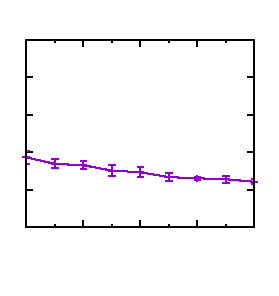
\includegraphics{Histo-lock-local-128-itu-server}}%
    \gplfronttext
  \end{picture}%
\endgroup

		\caption{128 bytes}
	\end{subfigure}
	\caption{The histogram problem on the xeon platform. Each plot uses a
	different amount of padding between the locks (specified beneath each
	plot). The plots show the running time of the histogram problem (each
	tick is 100 milliseconds. The axis starts at 0) as a function of the amount of padding between
	the histogram buckets in bytes.}
\end{figure}


\subsubsection{Compare-and-swap}
Following the same strategy as the fine-grained locking version implementation
above, we can use optimistic concurrency to implement a lock-free version of
the histogram.

Optimistic compare-and-swap works best when the operation we perform is cheap,
and the resource we perform it on has low contended. That way, retries will
happen rarely, and be cheap when they do.

The histogram problem lends itself well to a compare-and-swap based solution:
All writes to shared data are the results of simple increment operations, which
are fast. Resource contention depends on the ratio of locks to threads, and the
order of the input.

\begin{code}
\begin{Verbatim}[frame=single]
  private AtomicIntegerArray counters = ...;
  let taskCount parallel tasks do {
    final int from = ..., to = ...;
    for(int j = from; j < to; ++j) {
        counters.getAndIncrement(inputSequence[j]);
    }
  }
\end{Verbatim}
	\caption{Simplified code for the threads in the compare-and-swap 
	version of the histogram builder.}
	\label{code:histo-cas}
\end{code}

Code snippet \ref{code:histo-cas} outlines the compare-and-swap implementation
of the histogram builder. It uses Java's \java{AtomicIntegerArray} class to
hold counters. The \java{getAndIncrement} method performs the compare-and-swap
operation, and guarantees that updates are visible.

Reading the source code for the OpenJDK implementation of the
\java{AtomicIntegerArray} class \cite{atomicinterarraysrc} reveals that
the integers are stored in a plain \java{int} array.
To ensure atomicity and visibility of updates, the implementation relies on the
undocumented \java{sun.misc.Unsafe} class. This strongly suggests that our
implementation suffers from false sharing of cache lines, as the array elements
appear to be unpadded.

Figures \ref{fig:histo-cas-i5}, \ref{fig:histo-cas-i7}, and
\ref{fig:histo-cas-xeon} show that the execution time of this version of the
histogram builder improves drastically when we introduce padding between the
counters, confirming our suspicions that the \java{AtomicIntegerArray} class,
and therefore our histogram builder, suffers from false sharing.

\begin{figure}[hbtp]
	\centering
	\begin{tabular}{l r r}
		\hline
		\hline
		Platform & Best time (ms) & Padding (bytes)\\
		\hline
		i5 & 60.62 & 48 \\
		i7 & 25.26 & 128 \\
		Xeon & 48.62 & 128 \\
		\hline
		\hline
	\end{tabular}
	\caption{The best execution times for the compare-and-swap histogram
	builder, and the amounts of padding used to achieve them. Times
	are wall-clock execution times.}
	\label{table:histo-cas}
\end{figure}

The best execution times, shown in figure \ref{table:histo-cas}, are 
better than those of the fine-grained locking implementation by factors of 1.9,
2.8, and 8.7 for the i5, i7, and Xeon platforms respectively. However, the
communication-free implementation is still 3.3, 3.3, and 9.7 times faster than
the compare-and-swap version.

The lesson here is that data-sharing between cores should be avoided
entirely when doing so is easy. And when it cannot easily be avoided, we
should at least avoid unnecessary communication caused by false sharing.

\begin{figure}[hbpt]
\graphicspath{{plots/}}
% GNUPLOT: LaTeX picture with Postscript
\begingroup
  \makeatletter
  \providecommand\color[2][]{%
    \GenericError{(gnuplot) \space\space\space\@spaces}{%
      Package color not loaded in conjunction with
      terminal option `colourtext'%
    }{See the gnuplot documentation for explanation.%
    }{Either use 'blacktext' in gnuplot or load the package
      color.sty in LaTeX.}%
    \renewcommand\color[2][]{}%
  }%
  \providecommand\includegraphics[2][]{%
    \GenericError{(gnuplot) \space\space\space\@spaces}{%
      Package graphicx or graphics not loaded%
    }{See the gnuplot documentation for explanation.%
    }{The gnuplot epslatex terminal needs graphicx.sty or graphics.sty.}%
    \renewcommand\includegraphics[2][]{}%
  }%
  \providecommand\rotatebox[2]{#2}%
  \@ifundefined{ifGPcolor}{%
    \newif\ifGPcolor
    \GPcolorfalse
  }{}%
  \@ifundefined{ifGPblacktext}{%
    \newif\ifGPblacktext
    \GPblacktexttrue
  }{}%
  % define a \g@addto@macro without @ in the name:
  \let\gplgaddtomacro\g@addto@macro
  % define empty templates for all commands taking text:
  \gdef\gplbacktext{}%
  \gdef\gplfronttext{}%
  \makeatother
  \ifGPblacktext
    % no textcolor at all
    \def\colorrgb#1{}%
    \def\colorgray#1{}%
  \else
    % gray or color?
    \ifGPcolor
      \def\colorrgb#1{\color[rgb]{#1}}%
      \def\colorgray#1{\color[gray]{#1}}%
      \expandafter\def\csname LTw\endcsname{\color{white}}%
      \expandafter\def\csname LTb\endcsname{\color{black}}%
      \expandafter\def\csname LTa\endcsname{\color{black}}%
      \expandafter\def\csname LT0\endcsname{\color[rgb]{1,0,0}}%
      \expandafter\def\csname LT1\endcsname{\color[rgb]{0,1,0}}%
      \expandafter\def\csname LT2\endcsname{\color[rgb]{0,0,1}}%
      \expandafter\def\csname LT3\endcsname{\color[rgb]{1,0,1}}%
      \expandafter\def\csname LT4\endcsname{\color[rgb]{0,1,1}}%
      \expandafter\def\csname LT5\endcsname{\color[rgb]{1,1,0}}%
      \expandafter\def\csname LT6\endcsname{\color[rgb]{0,0,0}}%
      \expandafter\def\csname LT7\endcsname{\color[rgb]{1,0.3,0}}%
      \expandafter\def\csname LT8\endcsname{\color[rgb]{0.5,0.5,0.5}}%
    \else
      % gray
      \def\colorrgb#1{\color{black}}%
      \def\colorgray#1{\color[gray]{#1}}%
      \expandafter\def\csname LTw\endcsname{\color{white}}%
      \expandafter\def\csname LTb\endcsname{\color{black}}%
      \expandafter\def\csname LTa\endcsname{\color{black}}%
      \expandafter\def\csname LT0\endcsname{\color{black}}%
      \expandafter\def\csname LT1\endcsname{\color{black}}%
      \expandafter\def\csname LT2\endcsname{\color{black}}%
      \expandafter\def\csname LT3\endcsname{\color{black}}%
      \expandafter\def\csname LT4\endcsname{\color{black}}%
      \expandafter\def\csname LT5\endcsname{\color{black}}%
      \expandafter\def\csname LT6\endcsname{\color{black}}%
      \expandafter\def\csname LT7\endcsname{\color{black}}%
      \expandafter\def\csname LT8\endcsname{\color{black}}%
    \fi
  \fi
    \setlength{\unitlength}{0.0500bp}%
    \ifx\gptboxheight\undefined%
      \newlength{\gptboxheight}%
      \newlength{\gptboxwidth}%
      \newsavebox{\gptboxtext}%
    \fi%
    \setlength{\fboxrule}{0.5pt}%
    \setlength{\fboxsep}{1pt}%
\begin{picture}(7200.00,5040.00)%
    \gplgaddtomacro\gplbacktext{%
      \csname LTb\endcsname%%
      \put(528,500){\makebox(0,0)[r]{\strut{}$0$}}%
      \put(528,1220){\makebox(0,0)[r]{\strut{}$2\times10^{7}$}}%
      \put(528,1940){\makebox(0,0)[r]{\strut{}$4\times10^{7}$}}%
      \put(528,2660){\makebox(0,0)[r]{\strut{}$6\times10^{7}$}}%
      \put(528,3379){\makebox(0,0)[r]{\strut{}$8\times10^{7}$}}%
      \put(528,4099){\makebox(0,0)[r]{\strut{}$1\times10^{8}$}}%
      \put(528,4819){\makebox(0,0)[r]{\strut{}$1.2\times10^{8}$}}%
      \put(660,368){\rotatebox{-45}{\makebox(0,0)[l]{\strut{}0}}}%
      \put(1395,368){\rotatebox{-45}{\makebox(0,0)[l]{\strut{}16}}}%
      \put(2130,368){\rotatebox{-45}{\makebox(0,0)[l]{\strut{}32}}}%
      \put(2865,368){\rotatebox{-45}{\makebox(0,0)[l]{\strut{}48}}}%
      \put(3600,368){\rotatebox{-45}{\makebox(0,0)[l]{\strut{}64}}}%
      \put(4334,368){\rotatebox{-45}{\makebox(0,0)[l]{\strut{}80}}}%
      \put(5069,368){\rotatebox{-45}{\makebox(0,0)[l]{\strut{}96}}}%
      \put(5804,368){\rotatebox{-45}{\makebox(0,0)[l]{\strut{}112}}}%
      \put(6539,368){\rotatebox{-45}{\makebox(0,0)[l]{\strut{}128}}}%
    }%
    \gplgaddtomacro\gplfronttext{%
    }%
    \gplbacktext
    \put(0,0){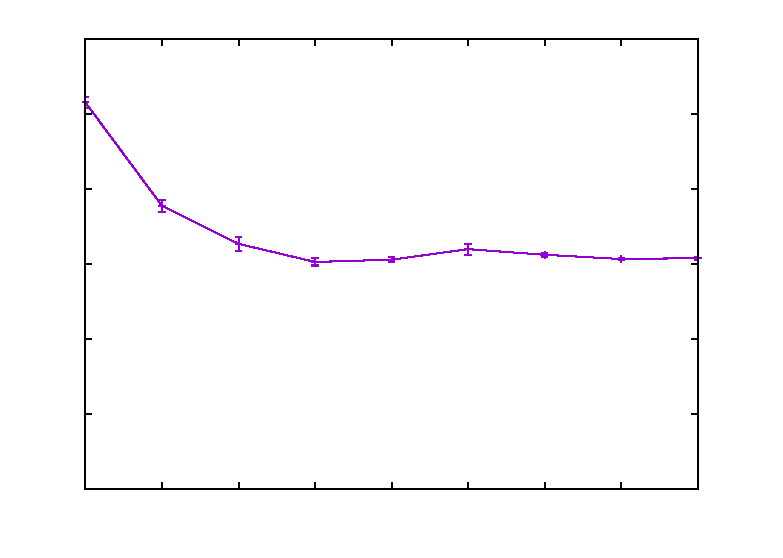
\includegraphics{histo-cas-i5}}%
    \gplfronttext
  \end{picture}%
\endgroup

\caption{Execution times for the compare-and-swap based histogram builder on the i5 platform. The plot shows the
	wall-clock execution time in ns., as a function of padding in bytes.}
\label{fig:histo-cas-i5}
\end{figure}

\begin{figure}[hbpt]
\graphicspath{{plots/}}
% GNUPLOT: LaTeX picture with Postscript
\begingroup
  \makeatletter
  \providecommand\color[2][]{%
    \GenericError{(gnuplot) \space\space\space\@spaces}{%
      Package color not loaded in conjunction with
      terminal option `colourtext'%
    }{See the gnuplot documentation for explanation.%
    }{Either use 'blacktext' in gnuplot or load the package
      color.sty in LaTeX.}%
    \renewcommand\color[2][]{}%
  }%
  \providecommand\includegraphics[2][]{%
    \GenericError{(gnuplot) \space\space\space\@spaces}{%
      Package graphicx or graphics not loaded%
    }{See the gnuplot documentation for explanation.%
    }{The gnuplot epslatex terminal needs graphicx.sty or graphics.sty.}%
    \renewcommand\includegraphics[2][]{}%
  }%
  \providecommand\rotatebox[2]{#2}%
  \@ifundefined{ifGPcolor}{%
    \newif\ifGPcolor
    \GPcolorfalse
  }{}%
  \@ifundefined{ifGPblacktext}{%
    \newif\ifGPblacktext
    \GPblacktexttrue
  }{}%
  % define a \g@addto@macro without @ in the name:
  \let\gplgaddtomacro\g@addto@macro
  % define empty templates for all commands taking text:
  \gdef\gplbacktext{}%
  \gdef\gplfronttext{}%
  \makeatother
  \ifGPblacktext
    % no textcolor at all
    \def\colorrgb#1{}%
    \def\colorgray#1{}%
  \else
    % gray or color?
    \ifGPcolor
      \def\colorrgb#1{\color[rgb]{#1}}%
      \def\colorgray#1{\color[gray]{#1}}%
      \expandafter\def\csname LTw\endcsname{\color{white}}%
      \expandafter\def\csname LTb\endcsname{\color{black}}%
      \expandafter\def\csname LTa\endcsname{\color{black}}%
      \expandafter\def\csname LT0\endcsname{\color[rgb]{1,0,0}}%
      \expandafter\def\csname LT1\endcsname{\color[rgb]{0,1,0}}%
      \expandafter\def\csname LT2\endcsname{\color[rgb]{0,0,1}}%
      \expandafter\def\csname LT3\endcsname{\color[rgb]{1,0,1}}%
      \expandafter\def\csname LT4\endcsname{\color[rgb]{0,1,1}}%
      \expandafter\def\csname LT5\endcsname{\color[rgb]{1,1,0}}%
      \expandafter\def\csname LT6\endcsname{\color[rgb]{0,0,0}}%
      \expandafter\def\csname LT7\endcsname{\color[rgb]{1,0.3,0}}%
      \expandafter\def\csname LT8\endcsname{\color[rgb]{0.5,0.5,0.5}}%
    \else
      % gray
      \def\colorrgb#1{\color{black}}%
      \def\colorgray#1{\color[gray]{#1}}%
      \expandafter\def\csname LTw\endcsname{\color{white}}%
      \expandafter\def\csname LTb\endcsname{\color{black}}%
      \expandafter\def\csname LTa\endcsname{\color{black}}%
      \expandafter\def\csname LT0\endcsname{\color{black}}%
      \expandafter\def\csname LT1\endcsname{\color{black}}%
      \expandafter\def\csname LT2\endcsname{\color{black}}%
      \expandafter\def\csname LT3\endcsname{\color{black}}%
      \expandafter\def\csname LT4\endcsname{\color{black}}%
      \expandafter\def\csname LT5\endcsname{\color{black}}%
      \expandafter\def\csname LT6\endcsname{\color{black}}%
      \expandafter\def\csname LT7\endcsname{\color{black}}%
      \expandafter\def\csname LT8\endcsname{\color{black}}%
    \fi
  \fi
    \setlength{\unitlength}{0.0500bp}%
    \ifx\gptboxheight\undefined%
      \newlength{\gptboxheight}%
      \newlength{\gptboxwidth}%
      \newsavebox{\gptboxtext}%
    \fi%
    \setlength{\fboxrule}{0.5pt}%
    \setlength{\fboxsep}{1pt}%
\begin{picture}(7200.00,5040.00)%
    \gplgaddtomacro\gplbacktext{%
      \csname LTb\endcsname%%
      \put(528,500){\makebox(0,0)[r]{\strut{}$0$}}%
      \put(528,1220){\makebox(0,0)[r]{\strut{}$1\times10^{7}$}}%
      \put(528,1940){\makebox(0,0)[r]{\strut{}$2\times10^{7}$}}%
      \put(528,2660){\makebox(0,0)[r]{\strut{}$3\times10^{7}$}}%
      \put(528,3379){\makebox(0,0)[r]{\strut{}$4\times10^{7}$}}%
      \put(528,4099){\makebox(0,0)[r]{\strut{}$5\times10^{7}$}}%
      \put(528,4819){\makebox(0,0)[r]{\strut{}$6\times10^{7}$}}%
      \put(660,368){\rotatebox{-45}{\makebox(0,0)[l]{\strut{}0}}}%
      \put(1395,368){\rotatebox{-45}{\makebox(0,0)[l]{\strut{}16}}}%
      \put(2130,368){\rotatebox{-45}{\makebox(0,0)[l]{\strut{}32}}}%
      \put(2865,368){\rotatebox{-45}{\makebox(0,0)[l]{\strut{}48}}}%
      \put(3600,368){\rotatebox{-45}{\makebox(0,0)[l]{\strut{}64}}}%
      \put(4334,368){\rotatebox{-45}{\makebox(0,0)[l]{\strut{}80}}}%
      \put(5069,368){\rotatebox{-45}{\makebox(0,0)[l]{\strut{}96}}}%
      \put(5804,368){\rotatebox{-45}{\makebox(0,0)[l]{\strut{}112}}}%
      \put(6539,368){\rotatebox{-45}{\makebox(0,0)[l]{\strut{}128}}}%
    }%
    \gplgaddtomacro\gplfronttext{%
    }%
    \gplbacktext
    \put(0,0){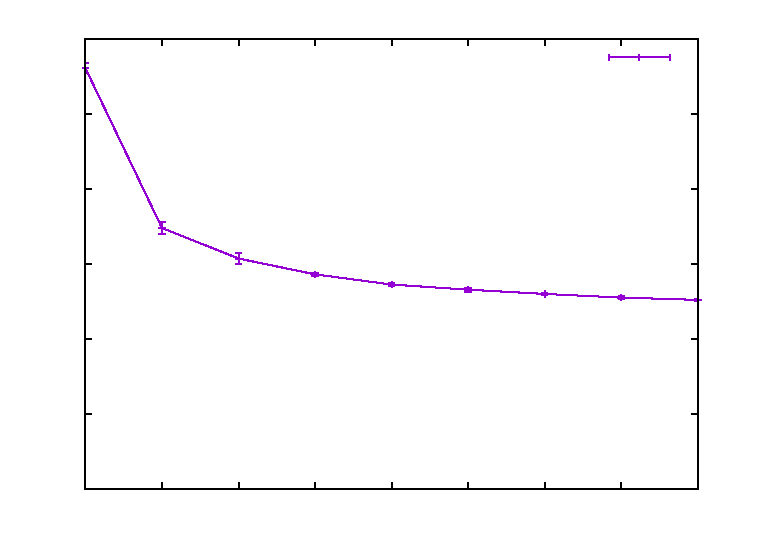
\includegraphics{histo-cas-i7}}%
    \gplfronttext
  \end{picture}%
\endgroup

\caption{Execution times for the compare-and-swap based histogram builder on the i7 platform. The plot shows the
	wall-clock execution time in ns., as a function of padding in bytes.}
	\label{fig:histo-cas-i7}
\end{figure}

\begin{figure}[hbpt]
\graphicspath{{plots/}}
% GNUPLOT: LaTeX picture with Postscript
\begingroup
  \makeatletter
  \providecommand\color[2][]{%
    \GenericError{(gnuplot) \space\space\space\@spaces}{%
      Package color not loaded in conjunction with
      terminal option `colourtext'%
    }{See the gnuplot documentation for explanation.%
    }{Either use 'blacktext' in gnuplot or load the package
      color.sty in LaTeX.}%
    \renewcommand\color[2][]{}%
  }%
  \providecommand\includegraphics[2][]{%
    \GenericError{(gnuplot) \space\space\space\@spaces}{%
      Package graphicx or graphics not loaded%
    }{See the gnuplot documentation for explanation.%
    }{The gnuplot epslatex terminal needs graphicx.sty or graphics.sty.}%
    \renewcommand\includegraphics[2][]{}%
  }%
  \providecommand\rotatebox[2]{#2}%
  \@ifundefined{ifGPcolor}{%
    \newif\ifGPcolor
    \GPcolorfalse
  }{}%
  \@ifundefined{ifGPblacktext}{%
    \newif\ifGPblacktext
    \GPblacktexttrue
  }{}%
  % define a \g@addto@macro without @ in the name:
  \let\gplgaddtomacro\g@addto@macro
  % define empty templates for all commands taking text:
  \gdef\gplbacktext{}%
  \gdef\gplfronttext{}%
  \makeatother
  \ifGPblacktext
    % no textcolor at all
    \def\colorrgb#1{}%
    \def\colorgray#1{}%
  \else
    % gray or color?
    \ifGPcolor
      \def\colorrgb#1{\color[rgb]{#1}}%
      \def\colorgray#1{\color[gray]{#1}}%
      \expandafter\def\csname LTw\endcsname{\color{white}}%
      \expandafter\def\csname LTb\endcsname{\color{black}}%
      \expandafter\def\csname LTa\endcsname{\color{black}}%
      \expandafter\def\csname LT0\endcsname{\color[rgb]{1,0,0}}%
      \expandafter\def\csname LT1\endcsname{\color[rgb]{0,1,0}}%
      \expandafter\def\csname LT2\endcsname{\color[rgb]{0,0,1}}%
      \expandafter\def\csname LT3\endcsname{\color[rgb]{1,0,1}}%
      \expandafter\def\csname LT4\endcsname{\color[rgb]{0,1,1}}%
      \expandafter\def\csname LT5\endcsname{\color[rgb]{1,1,0}}%
      \expandafter\def\csname LT6\endcsname{\color[rgb]{0,0,0}}%
      \expandafter\def\csname LT7\endcsname{\color[rgb]{1,0.3,0}}%
      \expandafter\def\csname LT8\endcsname{\color[rgb]{0.5,0.5,0.5}}%
    \else
      % gray
      \def\colorrgb#1{\color{black}}%
      \def\colorgray#1{\color[gray]{#1}}%
      \expandafter\def\csname LTw\endcsname{\color{white}}%
      \expandafter\def\csname LTb\endcsname{\color{black}}%
      \expandafter\def\csname LTa\endcsname{\color{black}}%
      \expandafter\def\csname LT0\endcsname{\color{black}}%
      \expandafter\def\csname LT1\endcsname{\color{black}}%
      \expandafter\def\csname LT2\endcsname{\color{black}}%
      \expandafter\def\csname LT3\endcsname{\color{black}}%
      \expandafter\def\csname LT4\endcsname{\color{black}}%
      \expandafter\def\csname LT5\endcsname{\color{black}}%
      \expandafter\def\csname LT6\endcsname{\color{black}}%
      \expandafter\def\csname LT7\endcsname{\color{black}}%
      \expandafter\def\csname LT8\endcsname{\color{black}}%
    \fi
  \fi
    \setlength{\unitlength}{0.0500bp}%
    \ifx\gptboxheight\undefined%
      \newlength{\gptboxheight}%
      \newlength{\gptboxwidth}%
      \newsavebox{\gptboxtext}%
    \fi%
    \setlength{\fboxrule}{0.5pt}%
    \setlength{\fboxsep}{1pt}%
\begin{picture}(7200.00,5040.00)%
    \gplgaddtomacro\gplbacktext{%
      \csname LTb\endcsname%%
      \put(528,500){\makebox(0,0)[r]{\strut{}$0$}}%
      \put(528,1040){\makebox(0,0)[r]{\strut{}$2\times10^{7}$}}%
      \put(528,1580){\makebox(0,0)[r]{\strut{}$4\times10^{7}$}}%
      \put(528,2120){\makebox(0,0)[r]{\strut{}$6\times10^{7}$}}%
      \put(528,2660){\makebox(0,0)[r]{\strut{}$8\times10^{7}$}}%
      \put(528,3199){\makebox(0,0)[r]{\strut{}$1\times10^{8}$}}%
      \put(528,3739){\makebox(0,0)[r]{\strut{}$1.2\times10^{8}$}}%
      \put(528,4279){\makebox(0,0)[r]{\strut{}$1.4\times10^{8}$}}%
      \put(528,4819){\makebox(0,0)[r]{\strut{}$1.6\times10^{8}$}}%
      \put(660,368){\rotatebox{-45}{\makebox(0,0)[l]{\strut{}0}}}%
      \put(1395,368){\rotatebox{-45}{\makebox(0,0)[l]{\strut{}16}}}%
      \put(2130,368){\rotatebox{-45}{\makebox(0,0)[l]{\strut{}32}}}%
      \put(2865,368){\rotatebox{-45}{\makebox(0,0)[l]{\strut{}48}}}%
      \put(3600,368){\rotatebox{-45}{\makebox(0,0)[l]{\strut{}64}}}%
      \put(4334,368){\rotatebox{-45}{\makebox(0,0)[l]{\strut{}80}}}%
      \put(5069,368){\rotatebox{-45}{\makebox(0,0)[l]{\strut{}96}}}%
      \put(5804,368){\rotatebox{-45}{\makebox(0,0)[l]{\strut{}112}}}%
      \put(6539,368){\rotatebox{-45}{\makebox(0,0)[l]{\strut{}128}}}%
    }%
    \gplgaddtomacro\gplfronttext{%
      \csname LTb\endcsname%%
      \put(5552,4646){\makebox(0,0)[r]{\strut{}histogram-cas-xeon}}%
    }%
    \gplbacktext
    \put(0,0){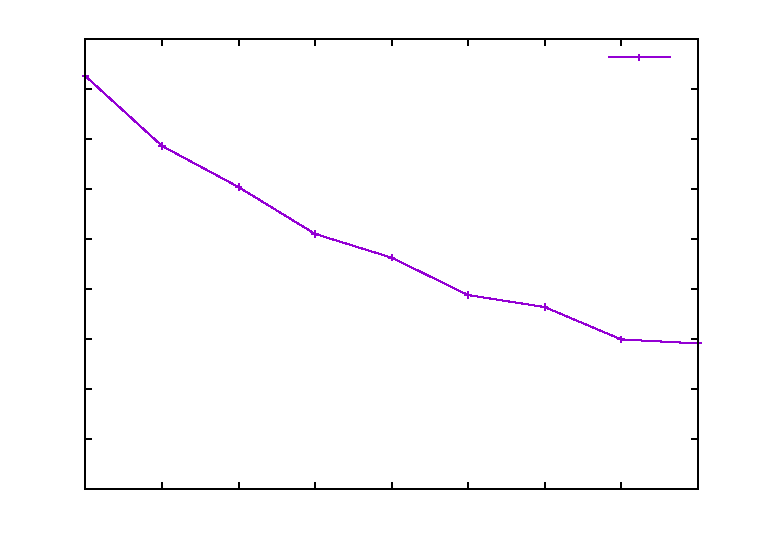
\includegraphics{histo-cas-xeon}}%
    \gplfronttext
  \end{picture}%
\endgroup

\caption{Execution times for the compare-and-swap based histogram builder on the Xeon platform. The plot shows the
	wall-clock execution time in ns., as a function of padding in bytes.}
	\label{fig:histo-cas-xeon}
\end{figure}

\subsection{Quicksort}
A famous example of a divide-and-conquer algorithm, Quicksort recursively
divides the sorting problem into independent subproblems, combining partial
results into a solution for the whole problem. We can see this problem division
as the same kind of avoidance we saw in the communication-free histogram
example: If the sub-problems are independent, they can be solved in parallel on
a multicore system without any communication between parallel processes. Of
course, we need to ensure that solutions are visible \textit{after} they are
found, but no communication is needed while the threads work. This is the only
of our experiments whare eliminating false sharing does not significantly
improve execution times.

\begin{code}
\begin{Verbatim}[frame=single]
  public class QuickSort extends RecursiveAction {
    ...
    protected void compute() {
      if (hi-lo <= cutoff) {
        SelectionSort.sort(array,lo,hi);
        return;
      }
      int mid = partition();
      ForkJoinTask<Void> leftTask =
        new QuickSort(array, lo, mid, cutoff).fork();
      QuickSort right =
        new QuickSort(array, mid + 1, hi, cutoff);
      right.compute();
      leftTask.join();
    }
    ...
  }
\end{Verbatim}
	\caption{Simplified code for the Quicksort problem. The left-out
	\java{SelectionSort.sort} method implements sequential Selection sort.
	The left-out \java{partition} method implements a median-of-three
	version of Hoare partitioning.}
	\label{code:qsort}
\end{code}

The experiments use a (somewhat naive) parallel implementation of quicksort,
outlined in code snippet \ref{code:qsort}.
Anytime the algorithm divides the problem in two, the calling thread forks a
task to solve the left part of the problem, executing the right part itself.
In this experiment we do not directly control the number of threads used on each
platform: Forked tasks are run in parallel at the discretion of the
\java{ForkJoinPool}.

As is common, and as is recommended in the popular algorithms text book by
\citet{sedgewick}, the implementation uses a cutoff to a sequential Selection
sort. An experiment is included to find a good value for the cutoff.

There is no step to combine the results of two subproblems, as calls operate
in-place on the same shared array. While this may \textit{seem} like communication
between threads, there is only a single thread operating on a given
array-segment at any time. The only relevant communication is that of the
constructor parameters to the recursive calls, and the reference to the array
itself. Operations in recursive calls are guaranteed to be visible to the caller
because of the call to \java{join()}.

\begin{figure}[hbpt]
\graphicspath{{plots/}}
% GNUPLOT: LaTeX picture with Postscript
\begingroup
  \makeatletter
  \providecommand\color[2][]{%
    \GenericError{(gnuplot) \space\space\space\@spaces}{%
      Package color not loaded in conjunction with
      terminal option `colourtext'%
    }{See the gnuplot documentation for explanation.%
    }{Either use 'blacktext' in gnuplot or load the package
      color.sty in LaTeX.}%
    \renewcommand\color[2][]{}%
  }%
  \providecommand\includegraphics[2][]{%
    \GenericError{(gnuplot) \space\space\space\@spaces}{%
      Package graphicx or graphics not loaded%
    }{See the gnuplot documentation for explanation.%
    }{The gnuplot epslatex terminal needs graphicx.sty or graphics.sty.}%
    \renewcommand\includegraphics[2][]{}%
  }%
  \providecommand\rotatebox[2]{#2}%
  \@ifundefined{ifGPcolor}{%
    \newif\ifGPcolor
    \GPcolorfalse
  }{}%
  \@ifundefined{ifGPblacktext}{%
    \newif\ifGPblacktext
    \GPblacktexttrue
  }{}%
  % define a \g@addto@macro without @ in the name:
  \let\gplgaddtomacro\g@addto@macro
  % define empty templates for all commands taking text:
  \gdef\gplbacktext{}%
  \gdef\gplfronttext{}%
  \makeatother
  \ifGPblacktext
    % no textcolor at all
    \def\colorrgb#1{}%
    \def\colorgray#1{}%
  \else
    % gray or color?
    \ifGPcolor
      \def\colorrgb#1{\color[rgb]{#1}}%
      \def\colorgray#1{\color[gray]{#1}}%
      \expandafter\def\csname LTw\endcsname{\color{white}}%
      \expandafter\def\csname LTb\endcsname{\color{black}}%
      \expandafter\def\csname LTa\endcsname{\color{black}}%
      \expandafter\def\csname LT0\endcsname{\color[rgb]{1,0,0}}%
      \expandafter\def\csname LT1\endcsname{\color[rgb]{0,1,0}}%
      \expandafter\def\csname LT2\endcsname{\color[rgb]{0,0,1}}%
      \expandafter\def\csname LT3\endcsname{\color[rgb]{1,0,1}}%
      \expandafter\def\csname LT4\endcsname{\color[rgb]{0,1,1}}%
      \expandafter\def\csname LT5\endcsname{\color[rgb]{1,1,0}}%
      \expandafter\def\csname LT6\endcsname{\color[rgb]{0,0,0}}%
      \expandafter\def\csname LT7\endcsname{\color[rgb]{1,0.3,0}}%
      \expandafter\def\csname LT8\endcsname{\color[rgb]{0.5,0.5,0.5}}%
    \else
      % gray
      \def\colorrgb#1{\color{black}}%
      \def\colorgray#1{\color[gray]{#1}}%
      \expandafter\def\csname LTw\endcsname{\color{white}}%
      \expandafter\def\csname LTb\endcsname{\color{black}}%
      \expandafter\def\csname LTa\endcsname{\color{black}}%
      \expandafter\def\csname LT0\endcsname{\color{black}}%
      \expandafter\def\csname LT1\endcsname{\color{black}}%
      \expandafter\def\csname LT2\endcsname{\color{black}}%
      \expandafter\def\csname LT3\endcsname{\color{black}}%
      \expandafter\def\csname LT4\endcsname{\color{black}}%
      \expandafter\def\csname LT5\endcsname{\color{black}}%
      \expandafter\def\csname LT6\endcsname{\color{black}}%
      \expandafter\def\csname LT7\endcsname{\color{black}}%
      \expandafter\def\csname LT8\endcsname{\color{black}}%
    \fi
  \fi
    \setlength{\unitlength}{0.0500bp}%
    \ifx\gptboxheight\undefined%
      \newlength{\gptboxheight}%
      \newlength{\gptboxwidth}%
      \newsavebox{\gptboxtext}%
    \fi%
    \setlength{\fboxrule}{0.5pt}%
    \setlength{\fboxsep}{1pt}%
\begin{picture}(7200.00,5040.00)%
    \gplgaddtomacro\gplbacktext{%
      \csname LTb\endcsname%%
      \put(858,440){\makebox(0,0)[r]{\strut{}$0$}}%
      \put(858,1170){\makebox(0,0)[r]{\strut{}$1\times10^{8}$}}%
      \put(858,1900){\makebox(0,0)[r]{\strut{}$2\times10^{8}$}}%
      \put(858,2630){\makebox(0,0)[r]{\strut{}$3\times10^{8}$}}%
      \put(858,3359){\makebox(0,0)[r]{\strut{}$4\times10^{8}$}}%
      \put(858,4089){\makebox(0,0)[r]{\strut{}$5\times10^{8}$}}%
      \put(858,4819){\makebox(0,0)[r]{\strut{}$6\times10^{8}$}}%
      \put(990,220){\makebox(0,0){\strut{}0}}%
      \put(1172,220){\makebox(0,0){\strut{}4}}%
      \put(1353,220){\makebox(0,0){\strut{}8}}%
      \put(1717,220){\makebox(0,0){\strut{}16}}%
      \put(2080,220){\makebox(0,0){\strut{}24}}%
      \put(2443,220){\makebox(0,0){\strut{}32}}%
      \put(3897,220){\makebox(0,0){\strut{}64}}%
      \put(4623,220){\makebox(0,0){\strut{}80}}%
      \put(6803,220){\makebox(0,0){\strut{}128}}%
    }%
    \gplgaddtomacro\gplfronttext{%
      \csname LTb\endcsname%%
      \put(5816,4646){\makebox(0,0)[r]{\strut{}padnone}}%
      \csname LTb\endcsname%%
      \put(5816,4426){\makebox(0,0)[r]{\strut{}padall}}%
      \csname LTb\endcsname%%
      \put(5816,4206){\makebox(0,0)[r]{\strut{}padsome}}%
    }%
    \gplbacktext
    \put(0,0){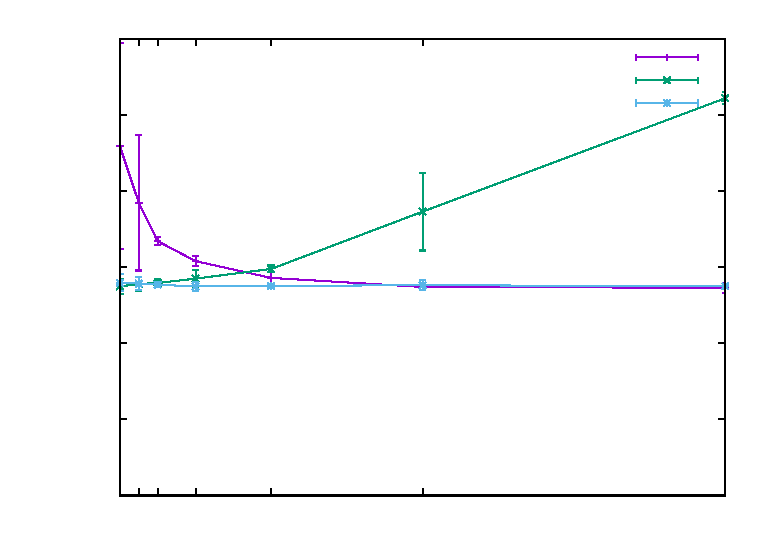
\includegraphics{qsort}}%
    \gplfronttext
  \end{picture}%
\endgroup

	\caption{Quicksort on the i5 platform. The plot shows wall-clock execution time in
	ns., as a function of padding in bytes. For the padnone experiment, the
	x-axis indicates the cutoff value in bytes.}
	\label{fig:qsort-i5}
\end{figure}

\begin{figure}[hbpt]
\graphicspath{{plots/}}
% GNUPLOT: LaTeX picture with Postscript
\begingroup
  \makeatletter
  \providecommand\color[2][]{%
    \GenericError{(gnuplot) \space\space\space\@spaces}{%
      Package color not loaded in conjunction with
      terminal option `colourtext'%
    }{See the gnuplot documentation for explanation.%
    }{Either use 'blacktext' in gnuplot or load the package
      color.sty in LaTeX.}%
    \renewcommand\color[2][]{}%
  }%
  \providecommand\includegraphics[2][]{%
    \GenericError{(gnuplot) \space\space\space\@spaces}{%
      Package graphicx or graphics not loaded%
    }{See the gnuplot documentation for explanation.%
    }{The gnuplot epslatex terminal needs graphicx.sty or graphics.sty.}%
    \renewcommand\includegraphics[2][]{}%
  }%
  \providecommand\rotatebox[2]{#2}%
  \@ifundefined{ifGPcolor}{%
    \newif\ifGPcolor
    \GPcolorfalse
  }{}%
  \@ifundefined{ifGPblacktext}{%
    \newif\ifGPblacktext
    \GPblacktexttrue
  }{}%
  % define a \g@addto@macro without @ in the name:
  \let\gplgaddtomacro\g@addto@macro
  % define empty templates for all commands taking text:
  \gdef\gplbacktext{}%
  \gdef\gplfronttext{}%
  \makeatother
  \ifGPblacktext
    % no textcolor at all
    \def\colorrgb#1{}%
    \def\colorgray#1{}%
  \else
    % gray or color?
    \ifGPcolor
      \def\colorrgb#1{\color[rgb]{#1}}%
      \def\colorgray#1{\color[gray]{#1}}%
      \expandafter\def\csname LTw\endcsname{\color{white}}%
      \expandafter\def\csname LTb\endcsname{\color{black}}%
      \expandafter\def\csname LTa\endcsname{\color{black}}%
      \expandafter\def\csname LT0\endcsname{\color[rgb]{1,0,0}}%
      \expandafter\def\csname LT1\endcsname{\color[rgb]{0,1,0}}%
      \expandafter\def\csname LT2\endcsname{\color[rgb]{0,0,1}}%
      \expandafter\def\csname LT3\endcsname{\color[rgb]{1,0,1}}%
      \expandafter\def\csname LT4\endcsname{\color[rgb]{0,1,1}}%
      \expandafter\def\csname LT5\endcsname{\color[rgb]{1,1,0}}%
      \expandafter\def\csname LT6\endcsname{\color[rgb]{0,0,0}}%
      \expandafter\def\csname LT7\endcsname{\color[rgb]{1,0.3,0}}%
      \expandafter\def\csname LT8\endcsname{\color[rgb]{0.5,0.5,0.5}}%
    \else
      % gray
      \def\colorrgb#1{\color{black}}%
      \def\colorgray#1{\color[gray]{#1}}%
      \expandafter\def\csname LTw\endcsname{\color{white}}%
      \expandafter\def\csname LTb\endcsname{\color{black}}%
      \expandafter\def\csname LTa\endcsname{\color{black}}%
      \expandafter\def\csname LT0\endcsname{\color{black}}%
      \expandafter\def\csname LT1\endcsname{\color{black}}%
      \expandafter\def\csname LT2\endcsname{\color{black}}%
      \expandafter\def\csname LT3\endcsname{\color{black}}%
      \expandafter\def\csname LT4\endcsname{\color{black}}%
      \expandafter\def\csname LT5\endcsname{\color{black}}%
      \expandafter\def\csname LT6\endcsname{\color{black}}%
      \expandafter\def\csname LT7\endcsname{\color{black}}%
      \expandafter\def\csname LT8\endcsname{\color{black}}%
    \fi
  \fi
    \setlength{\unitlength}{0.0500bp}%
    \ifx\gptboxheight\undefined%
      \newlength{\gptboxheight}%
      \newlength{\gptboxwidth}%
      \newsavebox{\gptboxtext}%
    \fi%
    \setlength{\fboxrule}{0.5pt}%
    \setlength{\fboxsep}{1pt}%
\begin{picture}(7200.00,5040.00)%
    \gplgaddtomacro\gplbacktext{%
      \csname LTb\endcsname%%
      \put(1122,440){\makebox(0,0)[r]{\strut{}$0$}}%
      \put(1122,927){\makebox(0,0)[r]{\strut{}$5\times10^{7}$}}%
      \put(1122,1413){\makebox(0,0)[r]{\strut{}$1\times10^{8}$}}%
      \put(1122,1900){\makebox(0,0)[r]{\strut{}$1.5\times10^{8}$}}%
      \put(1122,2386){\makebox(0,0)[r]{\strut{}$2\times10^{8}$}}%
      \put(1122,2873){\makebox(0,0)[r]{\strut{}$2.5\times10^{8}$}}%
      \put(1122,3359){\makebox(0,0)[r]{\strut{}$3\times10^{8}$}}%
      \put(1122,3846){\makebox(0,0)[r]{\strut{}$3.5\times10^{8}$}}%
      \put(1122,4332){\makebox(0,0)[r]{\strut{}$4\times10^{8}$}}%
      \put(1122,4819){\makebox(0,0)[r]{\strut{}$4.5\times10^{8}$}}%
      \put(1254,220){\makebox(0,0){\strut{}0}}%
      \put(1427,220){\makebox(0,0){\strut{}4}}%
      \put(1601,220){\makebox(0,0){\strut{}8}}%
      \put(1948,220){\makebox(0,0){\strut{}16}}%
      \put(2641,220){\makebox(0,0){\strut{}32}}%
      \put(4029,220){\makebox(0,0){\strut{}64}}%
      \put(6803,220){\makebox(0,0){\strut{}128}}%
    }%
    \gplgaddtomacro\gplfronttext{%
      \csname LTb\endcsname%%
      \put(5816,4646){\makebox(0,0)[r]{\strut{}padnone}}%
      \csname LTb\endcsname%%
      \put(5816,4426){\makebox(0,0)[r]{\strut{}padall}}%
      \csname LTb\endcsname%%
      \put(5816,4206){\makebox(0,0)[r]{\strut{}padsome}}%
    }%
    \gplbacktext
    \put(0,0){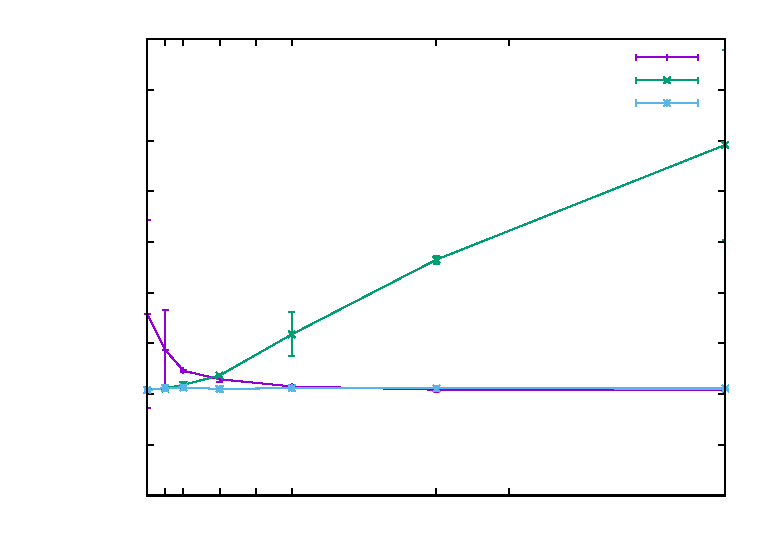
\includegraphics{qsort-desktop}}%
    \gplfronttext
  \end{picture}%
\endgroup

	\caption{Quicksort on the i7 platform. The plot shows wall-clock execution time in
	ns., as a function of padding in bytes. For the padnone experiment, the
	x-axis indicates the cutoff value in bytes.}
	\label{fig:qsort-i7}
\end{figure}

\begin{figure}[hbpt]
\graphicspath{{plots/}}
% GNUPLOT: LaTeX picture with Postscript
\begingroup
  \makeatletter
  \providecommand\color[2][]{%
    \GenericError{(gnuplot) \space\space\space\@spaces}{%
      Package color not loaded in conjunction with
      terminal option `colourtext'%
    }{See the gnuplot documentation for explanation.%
    }{Either use 'blacktext' in gnuplot or load the package
      color.sty in LaTeX.}%
    \renewcommand\color[2][]{}%
  }%
  \providecommand\includegraphics[2][]{%
    \GenericError{(gnuplot) \space\space\space\@spaces}{%
      Package graphicx or graphics not loaded%
    }{See the gnuplot documentation for explanation.%
    }{The gnuplot epslatex terminal needs graphicx.sty or graphics.sty.}%
    \renewcommand\includegraphics[2][]{}%
  }%
  \providecommand\rotatebox[2]{#2}%
  \@ifundefined{ifGPcolor}{%
    \newif\ifGPcolor
    \GPcolorfalse
  }{}%
  \@ifundefined{ifGPblacktext}{%
    \newif\ifGPblacktext
    \GPblacktexttrue
  }{}%
  % define a \g@addto@macro without @ in the name:
  \let\gplgaddtomacro\g@addto@macro
  % define empty templates for all commands taking text:
  \gdef\gplbacktext{}%
  \gdef\gplfronttext{}%
  \makeatother
  \ifGPblacktext
    % no textcolor at all
    \def\colorrgb#1{}%
    \def\colorgray#1{}%
  \else
    % gray or color?
    \ifGPcolor
      \def\colorrgb#1{\color[rgb]{#1}}%
      \def\colorgray#1{\color[gray]{#1}}%
      \expandafter\def\csname LTw\endcsname{\color{white}}%
      \expandafter\def\csname LTb\endcsname{\color{black}}%
      \expandafter\def\csname LTa\endcsname{\color{black}}%
      \expandafter\def\csname LT0\endcsname{\color[rgb]{1,0,0}}%
      \expandafter\def\csname LT1\endcsname{\color[rgb]{0,1,0}}%
      \expandafter\def\csname LT2\endcsname{\color[rgb]{0,0,1}}%
      \expandafter\def\csname LT3\endcsname{\color[rgb]{1,0,1}}%
      \expandafter\def\csname LT4\endcsname{\color[rgb]{0,1,1}}%
      \expandafter\def\csname LT5\endcsname{\color[rgb]{1,1,0}}%
      \expandafter\def\csname LT6\endcsname{\color[rgb]{0,0,0}}%
      \expandafter\def\csname LT7\endcsname{\color[rgb]{1,0.3,0}}%
      \expandafter\def\csname LT8\endcsname{\color[rgb]{0.5,0.5,0.5}}%
    \else
      % gray
      \def\colorrgb#1{\color{black}}%
      \def\colorgray#1{\color[gray]{#1}}%
      \expandafter\def\csname LTw\endcsname{\color{white}}%
      \expandafter\def\csname LTb\endcsname{\color{black}}%
      \expandafter\def\csname LTa\endcsname{\color{black}}%
      \expandafter\def\csname LT0\endcsname{\color{black}}%
      \expandafter\def\csname LT1\endcsname{\color{black}}%
      \expandafter\def\csname LT2\endcsname{\color{black}}%
      \expandafter\def\csname LT3\endcsname{\color{black}}%
      \expandafter\def\csname LT4\endcsname{\color{black}}%
      \expandafter\def\csname LT5\endcsname{\color{black}}%
      \expandafter\def\csname LT6\endcsname{\color{black}}%
      \expandafter\def\csname LT7\endcsname{\color{black}}%
      \expandafter\def\csname LT8\endcsname{\color{black}}%
    \fi
  \fi
    \setlength{\unitlength}{0.0500bp}%
    \ifx\gptboxheight\undefined%
      \newlength{\gptboxheight}%
      \newlength{\gptboxwidth}%
      \newsavebox{\gptboxtext}%
    \fi%
    \setlength{\fboxrule}{0.5pt}%
    \setlength{\fboxsep}{1pt}%
\begin{picture}(7200.00,5040.00)%
    \gplgaddtomacro\gplbacktext{%
      \csname LTb\endcsname%%
      \put(858,440){\makebox(0,0)[r]{\strut{}$0$}}%
      \put(858,1170){\makebox(0,0)[r]{\strut{}$1\times10^{8}$}}%
      \put(858,1900){\makebox(0,0)[r]{\strut{}$2\times10^{8}$}}%
      \put(858,2630){\makebox(0,0)[r]{\strut{}$3\times10^{8}$}}%
      \put(858,3359){\makebox(0,0)[r]{\strut{}$4\times10^{8}$}}%
      \put(858,4089){\makebox(0,0)[r]{\strut{}$5\times10^{8}$}}%
      \put(858,4819){\makebox(0,0)[r]{\strut{}$6\times10^{8}$}}%
      \put(990,220){\makebox(0,0){\strut{}0}}%
      \put(1172,220){\makebox(0,0){\strut{}4}}%
      \put(1353,220){\makebox(0,0){\strut{}8}}%
      \put(1717,220){\makebox(0,0){\strut{}16}}%
      \put(2443,220){\makebox(0,0){\strut{}32}}%
      \put(3897,220){\makebox(0,0){\strut{}64}}%
      \put(6803,220){\makebox(0,0){\strut{}128}}%
    }%
    \gplgaddtomacro\gplfronttext{%
      \csname LTb\endcsname%%
      \put(5816,4646){\makebox(0,0)[r]{\strut{}padnone}}%
      \csname LTb\endcsname%%
      \put(5816,4426){\makebox(0,0)[r]{\strut{}padall}}%
      \csname LTb\endcsname%%
      \put(5816,4206){\makebox(0,0)[r]{\strut{}padsome}}%
    }%
    \gplbacktext
    \put(0,0){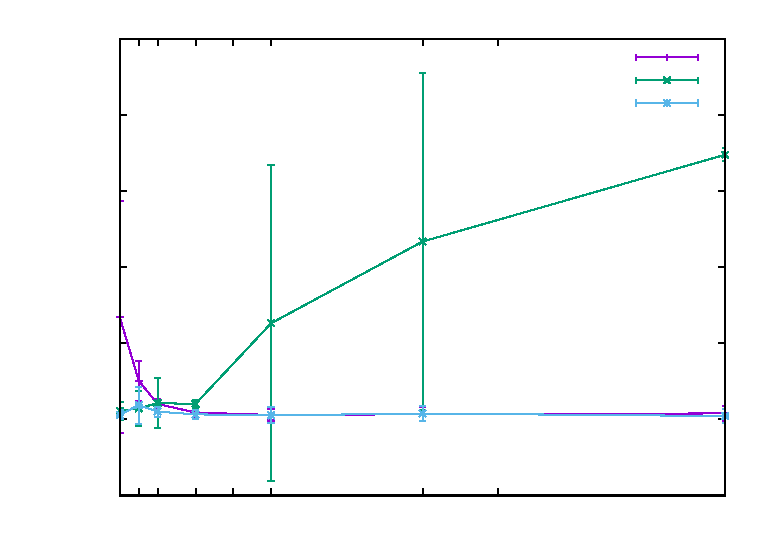
\includegraphics{qsort-server}}%
    \gplfronttext
  \end{picture}%
\endgroup

	\caption{Quicksort on the Xeon platform. The plot shows wall-clock execution time in
	ns., as a function of padding in bytes. For the padnone experiment, the
	x-axis indicates the cutoff value in bytes.}
	\label{fig:qsort-xeon}
\end{figure}

There is a risk of false-sharing every time the algorithm subdivides the input
array: The rightmost elements of the left part may share a cache line with the
leftmost elements of the right part. We run three experiments on each platform:
\begin{description}
	\item[padnone] With no padding, used to determine a good value for the cutoff.
	\item[padall] Where padding is added between all elements in the input
		array.
	\item[padsome] Where padding is added between some elements in the input
		array, such that padding segments and data segments are of equal
		length.
\end{description}

Experiments are run using an array with 4 million integers to be sorted. Padall
and padsome experiments use a cutoff value of 16 array elements, corresponding
to 64 bytes. Figures \ref{fig:qsort-i5}, \ref{fig:qsort-i7},
\ref{fig:qsort-xeon} show the execution times of the experiments. The results
show that adding padding between all array elements vastly increases execution
time, while adding padding between just some elements decrease execution time by
0-1.8\%

There are a few reasons why false sharing might not introduce significant
communication overhead to the Quicksort implementation: At most one cache line 
can be falsely shared at each problem division. This means each task
accesses at most 2 cache-lines that are falsely shared with other threads. An
additional two cache lines per task may be subject
to false invalidations due to the L2 prefetcher, as explained in
section \ref{sec:fine-grained-histo}. Each task writes to each of their array
elements at most once, either in the partitioning step, or when performing
Selection sort, so the shared cache lines suffer little contention, if any.
Finally, nothing guarantees visibility of updates before a task has finished, so
we do not suffer the full overhead of the cache coherence protocol.

The fact that we see slight improvement from padding in the padsome experiments
might simply be noise, but it leads us to a new question. The experiments are
all but guaranteed to have useless padding. That is, padding between elements
that are always in the same subdivisions. With Quicksort, we cannot predict
where the array will be divided beforehand, but perhaps other divide-and-conquer
algorithms, such as Mergesort, could benefit more from eliminating false
sharing, simply because we could add padding only in positions where the input
array gets split.

\subsection{K-means}
The K-means problem from the 2017 PCPP exam -- the original inspiration for
\textit{A multicore performance mystery solved}\cite{mystery} and this report --
is another example of a locking application which suffers from false sharing.

The k-means clustering algorithm takes as input: A list of points to be
clustered, and a list of $k$ initial cluster means. The algorithm then
assigns each point to its nearest cluster, and updates the clusters'
means according to the new assignments. This process is repeated iteratively
until cluster means have stabilised.

All our k-means experiments are run with 200.000 points and 81 clusters, and
take 108 iterations to complete.

\begin{code}
\begin{Verbatim}[frame=single]
  public static class Cluster implements Cluster{
    private volatile Point mean;
    private double sumx, sumy;
    private int count;
    public synchronized void addToMean(Point p) {
      sumx += p.x;
      sumy += p.y;
      count++;
    }
    public synchronized boolean computeNewMean() {
      ...
    }
\end{Verbatim}
	\caption{Simplified code for the k-means \java{Cluster} class}
	\label{code:cluster}
\end{code}

\begin{code}
\begin{Verbatim}[frame=single]
  while (!converged) {
    // Assignment step: put each point in exactly one
    // cluster
    let taskCount parallel tasks do {
      final int from = ..., to = ...;
      for (int pi=from; pi<to; pi++) 
        myCluster[pi] = closest(points[pi], clusters);
    }
    // Update step: recompute mean of each cluster
    let taskCount parallel tasks do {
      for (int pi=from; pi<to; pi++)
        myCluster[pi].addToMean(points[pi]);
    }
    converged = true;
    for (NormalCluster c : clusters)
      converged &= c.computeNewMean();
  }
\end{Verbatim}
	\caption{Simplified code for the original k-means implementation, KMeans2P.}
	\label{code:kmeans2p}
\end{code}

\begin{code}
\begin{Verbatim}[frame=single]
  while (!converged) {
    // Assignment step: put each point in exactly one
    // cluster
    let taskCount parallel tasks do {
      final int from = ..., to = ...;
      for (int pi=from; pi<to; pi++)
        closest(points[pi], clusters)
          .addToMean(points[pi]);
    }
    // Update step: recompute mean of each cluster
    converged = true;
    for (Cluster c : clusters)
      converged &= c.computeNewMean();
  }

\end{Verbatim}
	\caption{Simplified code for the optimized k-means implementation, KMeans2Q.}
	\label{code:kmeans2q}
\end{code}

The code used for this experiment is the same as in \cite{mystery}, with small
adaptations. We examine 4 K-means implementations:

\begin{description}
	\item[KMeans2P] {The unoptimized implementation described
		in\cite{mystery} and outlined in code snippet
		\ref{code:kmeans2p}.}
	\item[KMeans2Q] {The optimized implementation described in \cite{mystery}
		and outlined in  code snippet \ref{code:kmeans2q}.}
	\item[KMeans2Q64] {The same as KMeans2Q, but with a \java{Cluster} class
		with two 64-byte padding segments.}
	\item[KMeans2Q128] {The same as KMeans2Q, but with a \java{Cluster} class
		with two 128-byte padding segments.}
\end{description}

The most significant false sharing overhead comes from the \java{sumx},
\java{sumy}, \java{count}, and \java{mean} fields in the \java{Cluster}
class (Hereinafter, we shall refer to these the former three of these fields as
the \textit{assignment fields}). To see the problem, we need to understand just
3 points:

\begin{enumerate}
	\item{Updates to the assignment and \java{mean} fields
		are guarded by a lock (the surrounding \java{Cluster} instance),
		and the \java{mean} field is declared \java{volatile}}. This
		means that the fields are subject to the cache coherence
		protocol: Writes to these fields will result in invalidation
		messages being sent to the other cores. Reads from \java{mean}
		will force the CPU core to process pending invalidations, which
		may result in later cache misses.
	\item {The \java{mean} fields might be in the same cache line as the
		assignment fields. The fields consist of an object pointer, two
		\java{doubles} and an \java{int}, taking up a total of 28
		bytes. The small memory footprint even makes it possible for
		two separate \java{Cluster} instances to have fields in the same
		cache line!}
	\item {Every call to the \java{closest} method reads the \java{mean}
		fields of \textit{every cluster}. Calls to the \java{closest}
		and \java{addToMean} methods are interleaved in KMeans2Q, which
		means writes to the assignment fields happen concurrently with
		reads from the \java{volatile mean} field.}
\end{enumerate}

This means that every write to the assignment fields runs the risk of causing
false cache misses on all other CPU cores, if the assignment fields falsely
share the cache lines of \java{mean} fields.

The padded versions of KMeans2Q arrange the fields so that the assignment fields
are together in a contiguous memory segment, with padding both before and after
that segment. That should guarantee that the \java{mean} field is never in the
same cache line as the three other fields. No padding is added between the
\java{sumx}, \java{sumy}, and \java{count} fields. These three fields are always
updated together, so we welcome the possibility of them being placed in the
same cache line.

\begin{figure}[hbtp]
	\centering
	\begin{tabular}{l r r}
		\hline
		\hline
		K-means version & Time (ms) & SD (\%) \\
		\hline
		\input{plots/peterskmeans-i5}
		\hline
		\hline
	\end{tabular}
	\caption{The k-means problem on the i5 platform, using 4 tasks. Time is
	the total wall-clock execution time, the standard deviation (SD) is
	given as the percentage of the execution time.}
	\label{table:kmeans-i5}
\end{figure}

\begin{figure}[hbtp]
	\centering
	\begin{tabular}{l r r}
		\hline
		\hline
		K-means version & Time (ms) & SD (\%) \\
		\hline
		\input{plots/peterskmeans-i7}
		\hline
		\hline
	\end{tabular}
	\caption{The k-means problem on the i7 platform, using 8 tasks.  Time is
	the total wall-clock execution time, the standard deviation (SD) is
	given as the percentage of the execution time.}
	\label{table:kmeans-i7}
\end{figure}

\begin{figure}[hbtp]
	\centering
	\begin{tabular}{l r r}
		\hline
		\hline
		K-means version & Time (ms) & SD (\%) \\
		\hline
		\input{plots/peterskmeans-xeon}
		\hline
		\hline
	\end{tabular}
	\caption{The k-means problem on the Xeon platform, using 48 tasks.
	Time is the total wall-clock execution time, the standard deviation (SD)
	is given as the percentage of the execution time.}
	\label{table:kmeans-xeon}
\end{figure}

The results, shown in figures \ref{table:kmeans-i5}, \ref{table:kmeans-i7}, and
\ref{table:kmeans-xeon}, show that false sharing has a significant effect on our 
k-means implementations. Particularly on the Xeon platform, where the KMeans2Q128
is 2.1 times faster than KMeans2Q. Curiously, the execution time doesn't get as
close to that of KMeans2P as in \citeauthor{mystery}'s experiments, even though
both experiments use two 128-byte padding segments in the \java{Cluster} class.

\subsection{Striped hashmap}
Another problem used in the PCPP course, concurrent hashmap data structures
provide a more interesting example of striped locking applications than the
histogram builder we examined earlier: Hashmaps serve as general key-value
stores, their sizes may change dynamically, and unlike histograms, reads
and writes to hashmaps are often interleaved.

We consider two versions of the striped hashmap: Striped map, and striped-write
map. Both versions are from the PCPP course, and both versions are examined in
\cite{mystery}. Howver, \cite{mystery} examines only the striped-write map
with respect to false sharing.

Both implementations follow the same overall strategy: Key-value pairs are
stored in buckets, chosen by hashing they key. Buckets are implemented as linked
lists, allowing a single bucket to hold multiple key-value pairs. This
takes care of hash collisions. Each bucket is assigned to a stripe, and each
stripe is associated with a single lock that guards operations on buckets in
that stripe.

The code included here is minimal. The hashmap implementations are still used as
exercises in the PCPP course, and I do not wish to deprive students of the
satisfaction of completing them. The full implementations are fairly intricate,
but to see the risk of false sharing overhead, we need only consider the data
structures they use internally.

We use a quasi thread-local counter as the stress pattern for our hashmap
experiments. Each thread reads its own segment of the input, and stores the sum
of the inputs in a shared hashmap. Each thread uses a unique thread-id as key
for its own counter. Whether the counters are effectively thread-local depends
on whether the thread-ids hash to buckets in the same stripe.
Experiments are run with 32 stripes on all platforms, regardless of thread
count. The input sequence consists of 33 million integers, divided evenly
between threads.

\begin{code}
\begin{Verbatim}[frame=single]
  let taskCount parallel tasks do {
      final int threadId = ...;
      final int to = ..., from = ... ;
      map.put(threadId, 0);
      for(int j = from; j < to; ++j) {
        int a = inputSequence[j];
        map.put(threadId, map.get(threadId) + num);
      }
      threads.add(t);
    }
\end{Verbatim}
	\caption{Simplified code for the quasi thread-local counter we use for
	the hashmap experiments.}
\end{code}

\begin{code}
\begin{Verbatim}[frame=single]
  public static class StripedMap<K,V> {
    private volatile ItemNode<K,V>[] buckets;
    private Object[] locks;
    private final int[] sizes;
    ...
  }
\end{Verbatim}
	\caption{The most significant fields in the StripedMap class.}
\end{code}

\subsubsection{Striped map}
The striped map relies on locking for both reading and writing operations (such
as \java{get} and \java{put}). This ensures mutual exclusion as well as
visibility of updates.

The elements of the \java{locks} array pose a risk of false sharing: An
\java{Object} instance takes up 16 bytes\footnotemark, which means we can fit
up to four locks in a single 64-byte cache line. Taking or releasing a lock can
then falsely invalidate three other locks in the caches of other CPU cores.

The \java{buckets} and \java{sizes} fields are also candidates for false
sharing, but are unlikely to cause significant overhead: Writes and reads to
these fields are protected by locks, so the contention of these fields is
bounded, and likely overshadowed, by the contention of the locks.

\footnotetext{In chapter \ref{chap:javamem}, we saw that this is the case on our
three platforms, but it depends on the specific Java runtime platform.}

Figures \ref{fig:hashmap-striped-i5} and \ref{fig:hashmap-striped-i7-xeon} show
the wall-clock execution time when using the striped hashmap with different
amounts of padding between the locks.

\begin{code}
\begin{Verbatim}[frame=single]
  public static class StripedWriteMap<K,V> {
    private volatile ItemNode<K,V>[] buckets;
    private Object[] locks;
    private AtomicIntegerArray sizes;
    ...
  }
\end{Verbatim}
	\caption{The most significant fields in the StripedWriteMap class.}
\end{code}

\subsubsection{Striped-write map}
The striped-write map works in much the same way as the striped map, except it
lowers lock contention by not taking locks for read operations like \java{get}.
Visibility of writes is guaranteed by piggy-backing on the visibility
guarantees of the \java{AtomicIntegerArray} class, used to store element-counts
for each bucket. One disadvantage of this technique is that the \java{sizes}
elements now effectively become \java{volatile}, causing a larger coherence
overhead.

Figure \ref{fig:hashmap-stripedwrite} shows the wall-clock execution time when
using the striped-write hashmap with different amounts of padding between the locks.

The experiments show that false sharing has a pronounced impact on both hashmaps
across all three platforms, as simply padding elements of shared datastructures
improve execution times.
The biggest improvement is with the striped-write map on the Xeon platform.
Here, using 112 bytes of padding reduces the execution time by 33\%. The
smallest improvement is with the striped hashmap on the i5 platform. Here, using
48 bytes of padding reduces the execution time by 17\%.

There is an interesting artifact in the results: The striped-write map performs
remarkably worse than the striped map in these experiments. This may be
explained by its use of an immutable implementation of the \java{ItemNode}
class: Each write allocates new nodes, incurring both the cost of the
allocations and of garbage collecting the old nodes. A stress pattern with a
higher ratio of read- to write write-operations (the ratio in our thread-local
counter is $\sim 1/1$) should benefit from using the striped-write map, as the
cost saved by not locking eclipses the cost of the extra allocations.

\begin{figure}[hbpt]
\graphicspath{{plots/}}
% GNUPLOT: LaTeX picture with Postscript
\begingroup
  \makeatletter
  \providecommand\color[2][]{%
    \GenericError{(gnuplot) \space\space\space\@spaces}{%
      Package color not loaded in conjunction with
      terminal option `colourtext'%
    }{See the gnuplot documentation for explanation.%
    }{Either use 'blacktext' in gnuplot or load the package
      color.sty in LaTeX.}%
    \renewcommand\color[2][]{}%
  }%
  \providecommand\includegraphics[2][]{%
    \GenericError{(gnuplot) \space\space\space\@spaces}{%
      Package graphicx or graphics not loaded%
    }{See the gnuplot documentation for explanation.%
    }{The gnuplot epslatex terminal needs graphicx.sty or graphics.sty.}%
    \renewcommand\includegraphics[2][]{}%
  }%
  \providecommand\rotatebox[2]{#2}%
  \@ifundefined{ifGPcolor}{%
    \newif\ifGPcolor
    \GPcolorfalse
  }{}%
  \@ifundefined{ifGPblacktext}{%
    \newif\ifGPblacktext
    \GPblacktexttrue
  }{}%
  % define a \g@addto@macro without @ in the name:
  \let\gplgaddtomacro\g@addto@macro
  % define empty templates for all commands taking text:
  \gdef\gplbacktext{}%
  \gdef\gplfronttext{}%
  \makeatother
  \ifGPblacktext
    % no textcolor at all
    \def\colorrgb#1{}%
    \def\colorgray#1{}%
  \else
    % gray or color?
    \ifGPcolor
      \def\colorrgb#1{\color[rgb]{#1}}%
      \def\colorgray#1{\color[gray]{#1}}%
      \expandafter\def\csname LTw\endcsname{\color{white}}%
      \expandafter\def\csname LTb\endcsname{\color{black}}%
      \expandafter\def\csname LTa\endcsname{\color{black}}%
      \expandafter\def\csname LT0\endcsname{\color[rgb]{1,0,0}}%
      \expandafter\def\csname LT1\endcsname{\color[rgb]{0,1,0}}%
      \expandafter\def\csname LT2\endcsname{\color[rgb]{0,0,1}}%
      \expandafter\def\csname LT3\endcsname{\color[rgb]{1,0,1}}%
      \expandafter\def\csname LT4\endcsname{\color[rgb]{0,1,1}}%
      \expandafter\def\csname LT5\endcsname{\color[rgb]{1,1,0}}%
      \expandafter\def\csname LT6\endcsname{\color[rgb]{0,0,0}}%
      \expandafter\def\csname LT7\endcsname{\color[rgb]{1,0.3,0}}%
      \expandafter\def\csname LT8\endcsname{\color[rgb]{0.5,0.5,0.5}}%
    \else
      % gray
      \def\colorrgb#1{\color{black}}%
      \def\colorgray#1{\color[gray]{#1}}%
      \expandafter\def\csname LTw\endcsname{\color{white}}%
      \expandafter\def\csname LTb\endcsname{\color{black}}%
      \expandafter\def\csname LTa\endcsname{\color{black}}%
      \expandafter\def\csname LT0\endcsname{\color{black}}%
      \expandafter\def\csname LT1\endcsname{\color{black}}%
      \expandafter\def\csname LT2\endcsname{\color{black}}%
      \expandafter\def\csname LT3\endcsname{\color{black}}%
      \expandafter\def\csname LT4\endcsname{\color{black}}%
      \expandafter\def\csname LT5\endcsname{\color{black}}%
      \expandafter\def\csname LT6\endcsname{\color{black}}%
      \expandafter\def\csname LT7\endcsname{\color{black}}%
      \expandafter\def\csname LT8\endcsname{\color{black}}%
    \fi
  \fi
    \setlength{\unitlength}{0.0500bp}%
    \ifx\gptboxheight\undefined%
      \newlength{\gptboxheight}%
      \newlength{\gptboxwidth}%
      \newsavebox{\gptboxtext}%
    \fi%
    \setlength{\fboxrule}{0.5pt}%
    \setlength{\fboxsep}{1pt}%
\begin{picture}(7200.00,5040.00)%
    \gplgaddtomacro\gplbacktext{%
      \csname LTb\endcsname%%
      \put(858,500){\makebox(0,0)[r]{\strut{}$0$}}%
      \put(858,1040){\makebox(0,0)[r]{\strut{}$1\times10^{8}$}}%
      \put(858,1580){\makebox(0,0)[r]{\strut{}$2\times10^{8}$}}%
      \put(858,2120){\makebox(0,0)[r]{\strut{}$3\times10^{8}$}}%
      \put(858,2660){\makebox(0,0)[r]{\strut{}$4\times10^{8}$}}%
      \put(858,3199){\makebox(0,0)[r]{\strut{}$5\times10^{8}$}}%
      \put(858,3739){\makebox(0,0)[r]{\strut{}$6\times10^{8}$}}%
      \put(858,4279){\makebox(0,0)[r]{\strut{}$7\times10^{8}$}}%
      \put(858,4819){\makebox(0,0)[r]{\strut{}$8\times10^{8}$}}%
      \put(990,368){\rotatebox{45}{\makebox(0,0)[r]{\strut{}0}}}%
      \put(1717,368){\rotatebox{45}{\makebox(0,0)[r]{\strut{}16}}}%
      \put(2443,368){\rotatebox{45}{\makebox(0,0)[r]{\strut{}32}}}%
      \put(3170,368){\rotatebox{45}{\makebox(0,0)[r]{\strut{}48}}}%
      \put(3897,368){\rotatebox{45}{\makebox(0,0)[r]{\strut{}64}}}%
      \put(4623,368){\rotatebox{45}{\makebox(0,0)[r]{\strut{}80}}}%
      \put(5350,368){\rotatebox{45}{\makebox(0,0)[r]{\strut{}96}}}%
      \put(6076,368){\rotatebox{45}{\makebox(0,0)[r]{\strut{}112}}}%
      \put(6803,368){\rotatebox{45}{\makebox(0,0)[r]{\strut{}128}}}%
    }%
    \gplgaddtomacro\gplfronttext{%
      \csname LTb\endcsname%%
      \put(5816,4646){\makebox(0,0)[r]{\strut{}i5}}%
    }%
    \gplbacktext
    \put(0,0){\includegraphics{hashmap-striped-i5}}%
    \gplfronttext
  \end{picture}%
\endgroup

\caption{The striped hashmap problem on the i5 platform. The plot shows
	wall-clock execution time in ns., as a function of padding in bytes.}
\label{fig:hashmap-striped-i5}
\end{figure}

\begin{figure}[hbpt]
\graphicspath{{plots/}}
% GNUPLOT: LaTeX picture with Postscript
\begingroup
  \makeatletter
  \providecommand\color[2][]{%
    \GenericError{(gnuplot) \space\space\space\@spaces}{%
      Package color not loaded in conjunction with
      terminal option `colourtext'%
    }{See the gnuplot documentation for explanation.%
    }{Either use 'blacktext' in gnuplot or load the package
      color.sty in LaTeX.}%
    \renewcommand\color[2][]{}%
  }%
  \providecommand\includegraphics[2][]{%
    \GenericError{(gnuplot) \space\space\space\@spaces}{%
      Package graphicx or graphics not loaded%
    }{See the gnuplot documentation for explanation.%
    }{The gnuplot epslatex terminal needs graphicx.sty or graphics.sty.}%
    \renewcommand\includegraphics[2][]{}%
  }%
  \providecommand\rotatebox[2]{#2}%
  \@ifundefined{ifGPcolor}{%
    \newif\ifGPcolor
    \GPcolorfalse
  }{}%
  \@ifundefined{ifGPblacktext}{%
    \newif\ifGPblacktext
    \GPblacktexttrue
  }{}%
  % define a \g@addto@macro without @ in the name:
  \let\gplgaddtomacro\g@addto@macro
  % define empty templates for all commands taking text:
  \gdef\gplbacktext{}%
  \gdef\gplfronttext{}%
  \makeatother
  \ifGPblacktext
    % no textcolor at all
    \def\colorrgb#1{}%
    \def\colorgray#1{}%
  \else
    % gray or color?
    \ifGPcolor
      \def\colorrgb#1{\color[rgb]{#1}}%
      \def\colorgray#1{\color[gray]{#1}}%
      \expandafter\def\csname LTw\endcsname{\color{white}}%
      \expandafter\def\csname LTb\endcsname{\color{black}}%
      \expandafter\def\csname LTa\endcsname{\color{black}}%
      \expandafter\def\csname LT0\endcsname{\color[rgb]{1,0,0}}%
      \expandafter\def\csname LT1\endcsname{\color[rgb]{0,1,0}}%
      \expandafter\def\csname LT2\endcsname{\color[rgb]{0,0,1}}%
      \expandafter\def\csname LT3\endcsname{\color[rgb]{1,0,1}}%
      \expandafter\def\csname LT4\endcsname{\color[rgb]{0,1,1}}%
      \expandafter\def\csname LT5\endcsname{\color[rgb]{1,1,0}}%
      \expandafter\def\csname LT6\endcsname{\color[rgb]{0,0,0}}%
      \expandafter\def\csname LT7\endcsname{\color[rgb]{1,0.3,0}}%
      \expandafter\def\csname LT8\endcsname{\color[rgb]{0.5,0.5,0.5}}%
    \else
      % gray
      \def\colorrgb#1{\color{black}}%
      \def\colorgray#1{\color[gray]{#1}}%
      \expandafter\def\csname LTw\endcsname{\color{white}}%
      \expandafter\def\csname LTb\endcsname{\color{black}}%
      \expandafter\def\csname LTa\endcsname{\color{black}}%
      \expandafter\def\csname LT0\endcsname{\color{black}}%
      \expandafter\def\csname LT1\endcsname{\color{black}}%
      \expandafter\def\csname LT2\endcsname{\color{black}}%
      \expandafter\def\csname LT3\endcsname{\color{black}}%
      \expandafter\def\csname LT4\endcsname{\color{black}}%
      \expandafter\def\csname LT5\endcsname{\color{black}}%
      \expandafter\def\csname LT6\endcsname{\color{black}}%
      \expandafter\def\csname LT7\endcsname{\color{black}}%
      \expandafter\def\csname LT8\endcsname{\color{black}}%
    \fi
  \fi
    \setlength{\unitlength}{0.0500bp}%
    \ifx\gptboxheight\undefined%
      \newlength{\gptboxheight}%
      \newlength{\gptboxwidth}%
      \newsavebox{\gptboxtext}%
    \fi%
    \setlength{\fboxrule}{0.5pt}%
    \setlength{\fboxsep}{1pt}%
\begin{picture}(7200.00,5040.00)%
    \gplgaddtomacro\gplbacktext{%
      \csname LTb\endcsname%%
      \put(1122,500){\makebox(0,0)[r]{\strut{}$0$}}%
      \put(1122,1220){\makebox(0,0)[r]{\strut{}$5\times10^{7}$}}%
      \put(1122,1940){\makebox(0,0)[r]{\strut{}$1\times10^{8}$}}%
      \put(1122,2660){\makebox(0,0)[r]{\strut{}$1.5\times10^{8}$}}%
      \put(1122,3379){\makebox(0,0)[r]{\strut{}$2\times10^{8}$}}%
      \put(1122,4099){\makebox(0,0)[r]{\strut{}$2.5\times10^{8}$}}%
      \put(1122,4819){\makebox(0,0)[r]{\strut{}$3\times10^{8}$}}%
      \put(1254,368){\rotatebox{45}{\makebox(0,0)[r]{\strut{}0}}}%
      \put(1948,368){\rotatebox{45}{\makebox(0,0)[r]{\strut{}16}}}%
      \put(2641,368){\rotatebox{45}{\makebox(0,0)[r]{\strut{}32}}}%
      \put(3335,368){\rotatebox{45}{\makebox(0,0)[r]{\strut{}48}}}%
      \put(4029,368){\rotatebox{45}{\makebox(0,0)[r]{\strut{}64}}}%
      \put(4722,368){\rotatebox{45}{\makebox(0,0)[r]{\strut{}80}}}%
      \put(5416,368){\rotatebox{45}{\makebox(0,0)[r]{\strut{}96}}}%
      \put(6109,368){\rotatebox{45}{\makebox(0,0)[r]{\strut{}112}}}%
      \put(6803,368){\rotatebox{45}{\makebox(0,0)[r]{\strut{}128}}}%
    }%
    \gplgaddtomacro\gplfronttext{%
      \csname LTb\endcsname%%
      \put(5816,4646){\makebox(0,0)[r]{\strut{}i7}}%
      \csname LTb\endcsname%%
      \put(5816,4426){\makebox(0,0)[r]{\strut{}Xeon}}%
    }%
    \gplbacktext
    \put(0,0){\includegraphics{hashmap-striped-i7-xeon}}%
    \gplfronttext
  \end{picture}%
\endgroup

\caption{The striped hashmap problem on the i7 and Xeon platforms. The plot shows
	wall-clock execution time in ns., as a function of padding in bytes.}
\label{fig:hashmap-striped-i7-xeon}
\end{figure}

\begin{figure}[hbpt]
\graphicspath{{plots/}}
% GNUPLOT: LaTeX picture with Postscript
\begingroup
  \makeatletter
  \providecommand\color[2][]{%
    \GenericError{(gnuplot) \space\space\space\@spaces}{%
      Package color not loaded in conjunction with
      terminal option `colourtext'%
    }{See the gnuplot documentation for explanation.%
    }{Either use 'blacktext' in gnuplot or load the package
      color.sty in LaTeX.}%
    \renewcommand\color[2][]{}%
  }%
  \providecommand\includegraphics[2][]{%
    \GenericError{(gnuplot) \space\space\space\@spaces}{%
      Package graphicx or graphics not loaded%
    }{See the gnuplot documentation for explanation.%
    }{The gnuplot epslatex terminal needs graphicx.sty or graphics.sty.}%
    \renewcommand\includegraphics[2][]{}%
  }%
  \providecommand\rotatebox[2]{#2}%
  \@ifundefined{ifGPcolor}{%
    \newif\ifGPcolor
    \GPcolorfalse
  }{}%
  \@ifundefined{ifGPblacktext}{%
    \newif\ifGPblacktext
    \GPblacktexttrue
  }{}%
  % define a \g@addto@macro without @ in the name:
  \let\gplgaddtomacro\g@addto@macro
  % define empty templates for all commands taking text:
  \gdef\gplbacktext{}%
  \gdef\gplfronttext{}%
  \makeatother
  \ifGPblacktext
    % no textcolor at all
    \def\colorrgb#1{}%
    \def\colorgray#1{}%
  \else
    % gray or color?
    \ifGPcolor
      \def\colorrgb#1{\color[rgb]{#1}}%
      \def\colorgray#1{\color[gray]{#1}}%
      \expandafter\def\csname LTw\endcsname{\color{white}}%
      \expandafter\def\csname LTb\endcsname{\color{black}}%
      \expandafter\def\csname LTa\endcsname{\color{black}}%
      \expandafter\def\csname LT0\endcsname{\color[rgb]{1,0,0}}%
      \expandafter\def\csname LT1\endcsname{\color[rgb]{0,1,0}}%
      \expandafter\def\csname LT2\endcsname{\color[rgb]{0,0,1}}%
      \expandafter\def\csname LT3\endcsname{\color[rgb]{1,0,1}}%
      \expandafter\def\csname LT4\endcsname{\color[rgb]{0,1,1}}%
      \expandafter\def\csname LT5\endcsname{\color[rgb]{1,1,0}}%
      \expandafter\def\csname LT6\endcsname{\color[rgb]{0,0,0}}%
      \expandafter\def\csname LT7\endcsname{\color[rgb]{1,0.3,0}}%
      \expandafter\def\csname LT8\endcsname{\color[rgb]{0.5,0.5,0.5}}%
    \else
      % gray
      \def\colorrgb#1{\color{black}}%
      \def\colorgray#1{\color[gray]{#1}}%
      \expandafter\def\csname LTw\endcsname{\color{white}}%
      \expandafter\def\csname LTb\endcsname{\color{black}}%
      \expandafter\def\csname LTa\endcsname{\color{black}}%
      \expandafter\def\csname LT0\endcsname{\color{black}}%
      \expandafter\def\csname LT1\endcsname{\color{black}}%
      \expandafter\def\csname LT2\endcsname{\color{black}}%
      \expandafter\def\csname LT3\endcsname{\color{black}}%
      \expandafter\def\csname LT4\endcsname{\color{black}}%
      \expandafter\def\csname LT5\endcsname{\color{black}}%
      \expandafter\def\csname LT6\endcsname{\color{black}}%
      \expandafter\def\csname LT7\endcsname{\color{black}}%
      \expandafter\def\csname LT8\endcsname{\color{black}}%
    \fi
  \fi
    \setlength{\unitlength}{0.0500bp}%
    \ifx\gptboxheight\undefined%
      \newlength{\gptboxheight}%
      \newlength{\gptboxwidth}%
      \newsavebox{\gptboxtext}%
    \fi%
    \setlength{\fboxrule}{0.5pt}%
    \setlength{\fboxsep}{1pt}%
\begin{picture}(7200.00,5040.00)%
    \gplgaddtomacro\gplbacktext{%
      \csname LTb\endcsname%%
      \put(1122,500){\makebox(0,0)[r]{\strut{}$0$}}%
      \put(1122,1117){\makebox(0,0)[r]{\strut{}$5\times10^{8}$}}%
      \put(1122,1734){\makebox(0,0)[r]{\strut{}$1\times10^{9}$}}%
      \put(1122,2351){\makebox(0,0)[r]{\strut{}$1.5\times10^{9}$}}%
      \put(1122,2968){\makebox(0,0)[r]{\strut{}$2\times10^{9}$}}%
      \put(1122,3585){\makebox(0,0)[r]{\strut{}$2.5\times10^{9}$}}%
      \put(1122,4202){\makebox(0,0)[r]{\strut{}$3\times10^{9}$}}%
      \put(1122,4819){\makebox(0,0)[r]{\strut{}$3.5\times10^{9}$}}%
      \put(1254,368){\rotatebox{45}{\makebox(0,0)[r]{\strut{}0}}}%
      \put(1948,368){\rotatebox{45}{\makebox(0,0)[r]{\strut{}16}}}%
      \put(2641,368){\rotatebox{45}{\makebox(0,0)[r]{\strut{}32}}}%
      \put(3335,368){\rotatebox{45}{\makebox(0,0)[r]{\strut{}48}}}%
      \put(4029,368){\rotatebox{45}{\makebox(0,0)[r]{\strut{}64}}}%
      \put(4722,368){\rotatebox{45}{\makebox(0,0)[r]{\strut{}80}}}%
      \put(5416,368){\rotatebox{45}{\makebox(0,0)[r]{\strut{}96}}}%
      \put(6109,368){\rotatebox{45}{\makebox(0,0)[r]{\strut{}112}}}%
      \put(6803,368){\rotatebox{45}{\makebox(0,0)[r]{\strut{}128}}}%
    }%
    \gplgaddtomacro\gplfronttext{%
      \csname LTb\endcsname%%
      \put(5816,4646){\makebox(0,0)[r]{\strut{}i5}}%
      \csname LTb\endcsname%%
      \put(5816,4426){\makebox(0,0)[r]{\strut{}i7}}%
      \csname LTb\endcsname%%
      \put(5816,4206){\makebox(0,0)[r]{\strut{}Xeon}}%
    }%
    \gplbacktext
    \put(0,0){\includegraphics{hashmap-stripedwrite}}%
    \gplfronttext
  \end{picture}%
\endgroup

\caption{The striped-write hashmap problem on all 3 platforms. The plot shows
	wall-clock execution time in ns., as a function of padding in bytes.}
\label{fig:hashmap-stripedwrite}
\end{figure}
